
\documentclass[12pt,a4paper]{report}
  \usepackage[utf8]{inputenc}
  \usepackage[francais]{babel}
  \usepackage[T1]{fontenc}
  \usepackage{amsmath}
  \usepackage{amsfonts}
  \usepackage{amssymb}
  \usepackage{graphicx}
  \usepackage[left=2cm,right=2cm,top=2cm,bottom=2cm]{geometry}
  \usepackage{amsmath}
  \usepackage{textcomp}
  \usepackage{stmaryrd}
	\SetSymbolFont{stmry}{bold}{U}{stmry}{m}{n}
  \usepackage[Algorithme]{algorithm}
  \usepackage[center]{subfigure}
  \usepackage{algorithmic}
  \usepackage{color}
  \usepackage{listings}
  \usepackage[usenames,dvipsnames]{pstricks} % pour LaTeX Draw
%  \lstset{ 
%        language=Matlab,  % choose the language of the code
%%       basicstyle=10pt,  % the size of the fonts that are used for the code
%        numbers=left,     % where to put the line-numbers
%        numberstyle=\footnotesize,   % the size of the fonts that are used for the line-numbers
%        stepnumber=1,     % the step between two line-numbers. If it's 1 each line will be numbered
%        numbersep=5pt,    % how far the line-numbers are from the code
%%       backgroundcolor=\color{white},  % choose the background color. You must add \usepackage{color}
%        showspaces=false, % show spaces adding particular underscores
%        showstringspaces=false,      % underline spaces within strings
%        showtabs=false,   % show tabs within strings adding particular underscores
%%       frame=single,     % adds a frame around the code
%%       tabsize=2,        % sets default tabsize to 2 spaces
%%       captionpos=b,     % sets the caption-position to bottom
%        breaklines=true,  % sets automatic line breaking
%        breakatwhitespace=false,  % sets if automatic breaks should only happen at whitespace
%        escapeinside={\%*}{*)}    % if you want to add a comment within your code
%}
  \lstset {numbers=left,
	numberstyle=\tiny \bf,
	tabsize=4,
	language=matlab,
        basicstyle=\small,
        %upquote=true,
%        backgroundcolor=\color{gris},
        aboveskip={1.5\baselineskip},
        columns=fixed,
        showstringspaces=false,
        extendedchars=true,
        breaklines=true,
        prebreak = \raisebox{0ex}[0ex][0ex]{\ensuremath{\hookleftarrow}},
		frame=single,
        showtabs=false,
        showspaces=false,
        showstringspaces=false,
        identifierstyle=\ttfamily,
        keywordstyle=\color[rgb]{0,0,1},
        commentstyle=\color[rgb]{0.133,0.545,0.133},
        stringstyle=\color[rgb]{0.627,0.126,0.941},
		language=Java,
		captionpos=b,
		xleftmargin=8mm,
		xrightmargin=8mm}
  
  
% Environnement qui permet de modifier les marges localement
\newenvironment{changemargin}[2]{\begin{list}{}{%
\setlength{\topsep}{0pt}%
\setlength{\leftmargin}{0pt}%
\setlength{\rightmargin}{0pt}%
\setlength{\listparindent}{\parindent}%
\setlength{\itemindent}{\parindent}%
\setlength{\parsep}{0pt plus 1pt}%
\addtolength{\leftmargin}{#1}%
\addtolength{\rightmargin}{#2}%
}\item }{\end{list}}
%%\begin{changemargin}{0cm}{0cm}


 
\title{Mémoire de stage - Extension de la PGD à des problèmes de dynamique non-linéaires}
\author{Pierre \bsc{Nargil}}
\date{23 juin 2013}

\begin{document}

%\maLetitle
%\include{couverture/couvertureMax}
\thispagestyle{empty}
\enlargethispage{1cm}\vspace*{-2cm}
\noindent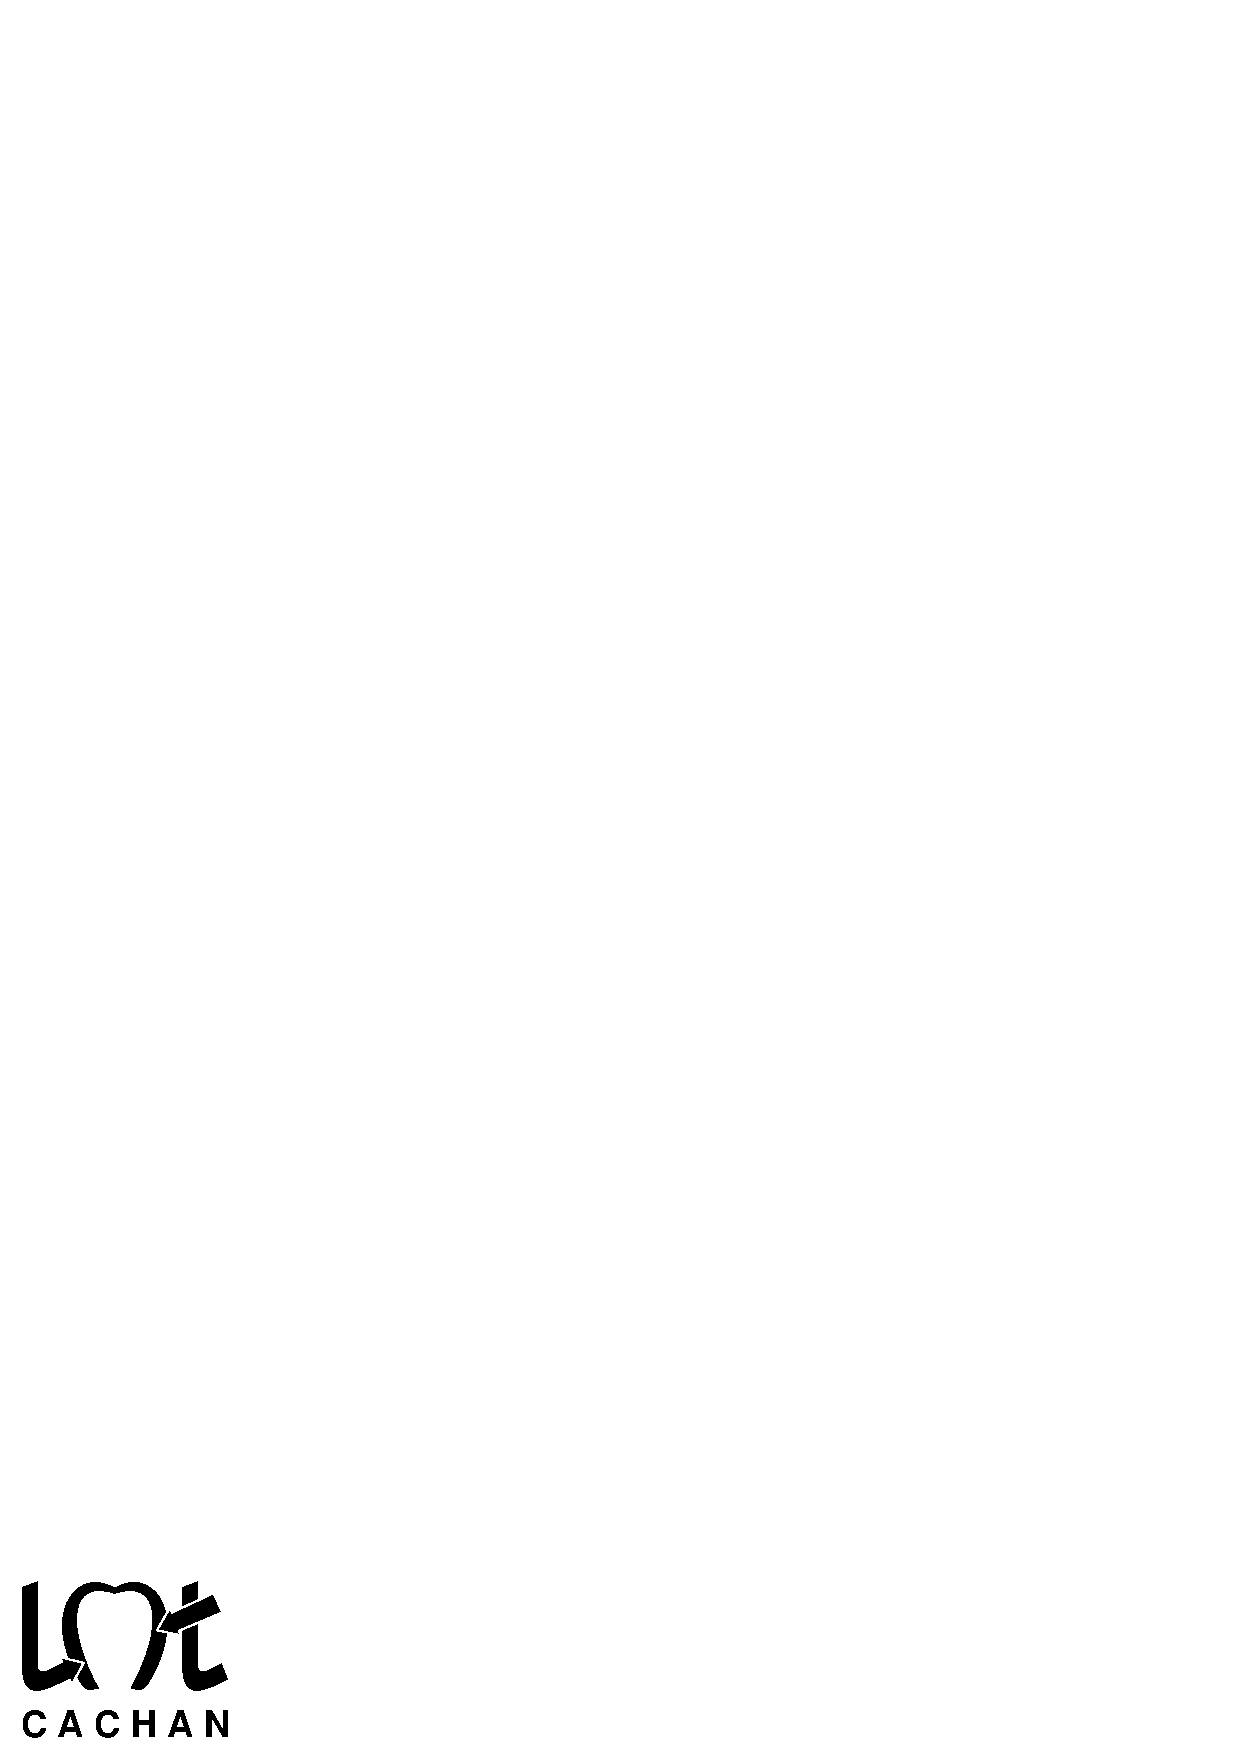
\includegraphics[height=2cm]{Images/logoLMT}
\hfill
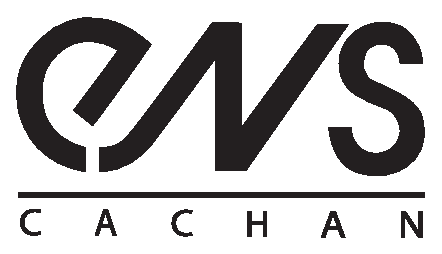
\includegraphics[height=1.6cm]{Images/ENS}
\par\noindent{\itshape\bfseries ENSC-2012/2013}
\begin{center}\normalfont\bfseries
\par\vspace{.5cm} BIBLIOGRAPHIE DE THÈSE \par DE L'ÉCOLE NORMALE SUPÉRIEURE DE CACHAN
\par\vspace{1cm} \textnormal{Présentée par}
\par\vspace{.5cm}\textnormal{\bfseries\Large Pierre \bsc{Nargil}}
\par\vspace{1cm} \textnormal{pour obtenir le diplôme de}
%\par\vspace{.5cm} DOCTEUR en MÉCANIQUE DES STRUCTURES
\par\vspace{.5cm} DOCTORAT en MÉCANIQUE DES STRUCTURES
%\par\vspace{1cm} \textnormal{Domaine}
%\par\vspace{.5cm} MÉCANIQUE
\par\vspace{\stretch{1}} \textnormal{Sujet de la thèse}
\par\vspace{.5cm} {\Large Extension de la PGD à des problèmes de dynamique non-linéaires}
\par\vspace{\stretch{1}}
\normalfont\normalsize 2013-2016, Encadré par :
\par\vspace{.5cm}\begin{tabular}{l@{\quad}l@{\quad}l}
  Pierre-Alain \bsc{Boucard} & Professeur des Universités, ENS Cachan \\
  Francois \bsc{Louf} & Maître de conférences, ENS Cachan \\
\end{tabular}
\par\vspace{\stretch{1}}
\textbf{LMT-Cachan}
\par\textnormal{ENS Cachan\,/\,CNRS\,/\,UPMC\,/\,PRES UniverSud Paris}
\par\textnormal{61 avenue du Président Wilson, F-94235 Cachan cedex, France}
\end{center}
\clearpage



\renewcommand{\contentsname}{Sommaire}
\tableofcontents
\renewcommand{\lstlistingname}{Code source}

  \setlength{\parskip}{0.2cm}
  \setlength{\leftskip}{1cm}
  \setlength{\rightskip}{1cm}

\chapter{Introduction}
L'objectif de ce travail est d'appliquer une méthode de résolution PGD (Proper Generalized Decomposition), qui est une méthode de réduction de modèles où la solution est à variables séparées, à des problèmes de dynamique présentant des non-linéarités. Ce rapport propose ici introduction à la PGD avec une présentation d'autres méthodes de réductions de modèles, tel que la condensation, la méthode de Rayleigh-Ritz et la POD.

\section{La réduction de modèles}
La résolution numérique de problèmes de mécanique fait partie intégrante du travail de la plupart des ingénieurs, et connaît évidemment des limitations. Ces résolutions représentent des calculs gourmands en ressources et en temps, et la volonté croissante des industriels de s'appuyer le plus souvent sur la simulation plutôt que sur l'essai, place l'amélioration des méthodes utilisées au cœur de la problématique de nombreuses recherches. Pour l'industriel le gain de temps est un enjeu majeur pour être concurrentiel, voire pour réduire le coût d'une étude et donc au final de son produit. Les méthodes de réductions de modèles tendent à simplifier le problème pour réduire sa taille. Elles sont basées sur une diminution de la dimension de l'espace de recherche des solutions. Ceci nécessite la construction d'une
base réduite. On peut alors distinguer parmi ces méthodes, celles qui nécessitent une connaissance préalable d'une solution pour construire la base sur laquelle le problème sera projeté, elles sont dites "a posteriori", de celles dites "a priori" qui construisent la base pendant le calcul de résolution. 

Parmi les méthodes "a posteriori" se trouve la POD (Proper Orthogonal Decomposition), qui a fait l'objet de nombreux travaux d'études ces vingt dernières années. Il s'agit d'une méthode basée sur la séparation de variables qui sera présentée plus en détail par la suite. 

Outre une amélioration du temps de résolution pour des calculs couramment effectués par les industriels, la réduction de modèle peut se montrer si efficace dans la diminution du temps de calcul que de nouvelles résolutions peuvent être envisagées. En effet l'industrie rencontre des problèmes de tailles telles qu'elle ne peut envisager de les résoudre pour des questions de temps, voire de limites des performances même des plus puissantes machines. La première possibilité apportée par une réduction de modèle est l'utilisation pour l'optimisation. Puisque même si les méthodes "a posteriori" entraînent une première résolution du problème par une méthode standard, elles permettent, une fois la base réduite obtenue, de faire une série de calculs rapides pouvant permettre une optimisation ou une étude de type Monte Carlo sur le modèle réduit.

\section{La PGD}
\subsection{Généralités}
La PGD, pour "Proper Generalized Decomposition" , trouve son origine dans \cite{LATIN1} sous le nom de "radial time-space approximation", comme faisant partie la méthode LATIN (voir également \cite{LATIN2}). 

Parmi les possibilités apportées par la réduction de modèles, elle peut permettre de résoudre des problèmes jusque là inenvisageable par exemple dans la chimie quantique (quand des processus chimiques impliquent un nombre de molécules de réactifs si petit que le concept de continuité de concentration n'est plus valide, par exemple dans la recherche génétique). De tels problèmes peuvent rapidement être impossibles à résoudre par des méthodes standards, car ils souffrent de ce que l'on appelle la malédiction de la dimension. La solution est inaccessible par des approches traditionnelles de discrétisation utilisant un maillage car elles présentent une taille du système à résoudre qui croit exponentiellement en fonction du nombre de particules. Plus de détail sur ce sujet sont donné dans \cite{Paradigm}.

La diminution drastique de temps de calcul apportée par la PGD permet d'envisager de nouvelles utilisations de la simulation, notamment dans les DDDAS (pour Dynamic Data-Driven Application System), dont l'enjeu est de permettre à la simulation d'interagir avec une manipulation en temps réel. C'est-à-dire que les instruments actionneurs seront influencés par les résultats de calculs apportés par la simulation et les capteurs du système renverront des données à la simulation pour réajuster les calculs. Les DDDAS sont un sujet d'études identifié par la USNSF (United States National Science Foundation) dans son rapport en 2006 sur les SBES (Simulation-based Engineering Sciences) comme étant parmi les cinq challenges majeurs de la prochaine décennie. Pour plus de détails sur la PGD dans le cadre des DDDAS le lecteur pourra consulter \cite{DDAS}.

La PDG rencontre donc un franc succès depuis quelques années et ses applications sont pléthores. Un aperçu des différents travaux concernant cette méthode peut être trouvé dans \cite{ShortReview}.

\subsection{Mise en place de nouvelles variables : nouvelles coordonnées}
La PGD présente un autre avantage, par la mise en place de coordonnées supplémentaires, comme le décrivent \cite{Paradigm} et \cite{DDAS}. Il s'agit de rajouter au produit de fonctions à variables séparées, une fonction d'une nouvelle variable. Ceci permet de conserver une variable comme une inconnue et ainsi d'avoir un problème résolu quelque soit la valeur de cette variable. Pour obtenir un tel résultat sans cette méthode il faudrait effectuer de nombreux tirages de valeurs pour la variable et réaliser une approche de Monte Carlo, ce qui requerrait autant de résolutions. L'ajout de cette coordonnée permet donc de passer outre la nécessité de la valeur d'une variable au calcul, ou de résoudre une famille de problèmes qui dépendent de cette variable. C'est le principe de base de l'analyse stochastique, qui fait l'objet d'un intérêt grandissant. De cette manière la résolution du problème par la PGD apporte plus encore qu'une résolution directe, et peut permettre facilement la mise en place d'une optimisation. Dans les articles cités précédemment, les auteurs présentent comme exemple un problème de thermique à résoudre pour lequel la conductivité matériau est inconnue. Mais ceci ne se limite pas à une valeur matériau et peut s'appliquer à une condition initiale ou à une valeur géométrique...

\chapter{Les méthodes de réduction de modèles}

Les notations dans ce rapport seront les suivantes (elles n'ont de sens que pour les élément discrétisé):
\begin{itemize}
\item pour un vecteur : $\mathbf{v}$ (en minuscule et gras)
\item pour un élément du vecteur $\mathbf{v}$ : $\text{v}_i$ 
								(en minuscule et non gras)
\item pour une matrice : $\mathbf{M}$ (en majuscule et gras)
\item pour un élément de la matrice $\mathbf{M}$ : $\text{M}_{ij}$ 
								(en majuscule et non gras)
\item pour un scalaire en minuscule et non gras.
\item $\mathbf{I}$ est la matrice identité.
\item $.^T$ est l'opérateur transposition.
\item $\delta_{..}$ et le symbole de Kronecker.
\end{itemize}

\noindent
Un problème de dynamique peut s'écrire sous la forme (pour le cas discret):
\begin{equation}
\label{PFD}
\mathbf{M}\mathbf{\ddot{u}} + \mathbf{C}\mathbf{\dot{u}} + \mathbf{K}\mathbf{u} =
\mathbf{f}
\end{equation}
\begin{itemize}
\item $\mathbf{M}$ est la matrice de masse
\item $\mathbf{C}$ est une matrice d'amortissement
\item $\mathbf{K}$ est une matrice de raideur
\item $\mathbf{u}$ est le vecteur contenant les déplacements aux nœuds
\item $\mathbf{f}$ est le vecteur les efforts extérieurs sur les nœuds
\end{itemize}

\paragraph{}
Il existe plusieurs méthodes de résolution, et celles de réductions de modèles se basent sur une projection du problème sur une base, pour en diminuer la taille.

\section{Condensation\label{SectionCondensation}}
La résolution classique à l'aide d'un modèle de discrétisation tel que les éléments finis se base sur une matrice dont la taille dépend de la finesse du maillage. Une géométrie complexe dans une zone d'intérêt nécessitera un raffinement qui entraîne un agrandissement du problème à résoudre. Avant de se lancer dans une résolution coûteuse, il peut être intéressant de réduire la taille du modèle en condensant les degrés de liberté possédant peu ou pas d'inertie et qui ne sont pas soumis à des efforts extérieurs. Les nœuds  amenés à être condensés sont appelés nœuds esclaves et ceux qui seront conservés sont appelés nœuds maîtres.

Le système se présente alors sous cette forme si l'on néglige l'inertie des nœuds esclaves:
\begin{equation}
\begin{bmatrix}
   \mathbf{M_{11}} & 0 \\
   0 & 0 \\
\end{bmatrix}
\begin{Bmatrix}
   \mathbf{\ddot{u}_1} \\
   \mathbf{\ddot{u}_2} \\
\end{Bmatrix}
+
\begin{bmatrix}
   \mathbf{K_{11}} & \mathbf{K_{12}} \\
   \mathbf{K_{21}} & \mathbf{K_{22}} \\
\end{bmatrix}
\begin{Bmatrix}
   \mathbf{u_1} \\
   \mathbf{u_2} \\
\end{Bmatrix}
=
\begin{Bmatrix}
   \mathbf{f_1} \\
   0 \\
\end{Bmatrix}
\end{equation}
Où $\mathbf{u_1}$ contient les degrés de libertés des nœuds maîtres et $\mathbf{u_2}$ ceux des nœuds esclaves. On obtient alors les deux équations :
\begin{equation}
\left\{
\begin{array}{r c l}
	\mathbf{M_{11}}   \mathbf{\ddot{u}_1}
	+ \mathbf{K_{11}} \mathbf{u_1}
	+ \mathbf{K_{12}} \mathbf{u_2}
	& = & 
	\mathbf{f}_{\mathbf{1}}
\\
	\mathbf{K}_{\mathbf{21}} \mathbf{u_1}
	+ \mathbf{K}_{\mathbf{22}} \mathbf{u_2}
	& = & 
	\mathbf{0}

\end{array}
\right.
\end{equation}

\noindent
On peut alors déterminer le comportement des nœuds esclaves à partir des nœuds maîtres ainsi :
\begin{equation}
\label{ApproximationGuyan}
	\mathbf{u_2} = \mathbf{K_{22}}^{-1}
								\mathbf{K_{21}}
								\mathbf{u_1}
\end{equation}

\noindent
Alors la résolution du système se réduit à :
\begin{equation}
	\mathbf{M_{11}} \mathbf{\ddot{u}_1}
	+ \left(
		\mathbf{K_{11}} \mathbf{u_1}
		- \mathbf{K_{12}}
			\mathbf{K_{22}}^{-1}
			\mathbf{K_{21}}
	  \right) \mathbf{u_1}
	= \mathbf{f_1}
\end{equation}
qui ne tient compte que des nœuds maîtres. La résolution du problème modifié par cette condensation apporte la solution exacte en statique, puisqu'alors l'inertie n'a pas de rôle. L'approximation apportée par la réduction de Guyan est de conserver la relation entre maîtres et esclaves \ref{ApproximationGuyan} même quand les seconds possèdent un peu d'inertie. On introduit $\mathbf{L}$:
\begin{equation}
\mathbf{u} 
= 
\begin{Bmatrix}
   \mathbf{\ddot{u}_1} \\
   \mathbf{\ddot{u}_2} \\
\end{Bmatrix}
=
\begin{bmatrix}
   \mathbf{I} \\
   \mathbf{K_{22}}^{-1}
	\mathbf{K_{21}} \\
\end{bmatrix}
\mathbf{u_1}
=
\mathbf{L}
\mathbf{u_1}
\end{equation}

\noindent
Le calcul de l'énergie cinétique et de l'énergie potentielle deviennent:
\begin{equation}
\left\{
	\begin{array}{r c c c c c l}
		e_c &=&
			\frac{1}{2} \mathbf{\ddot{u}} \mathbf{M} \mathbf{\ddot{u}}
			&=&
			\frac{1}{2} \mathbf{\ddot{u}}_{\mathbf{1}} \mathbf{L}^T
							\mathbf{M} \mathbf{L}
							\mathbf{\ddot{u}_1}
			&=&
			\frac{1}{2} \mathbf{\ddot{u}_1} 
							\mathbf{\hat{M}} \mathbf{\ddot{u}_1}
		\\
		e_p &=&
			\frac{1}{2} \mathbf{u} \mathbf{K} \mathbf{u}
			&=&
			\frac{1}{2} \mathbf{u_1} \mathbf{L}^T
							\mathbf{K} \mathbf{L} \mathbf{u_1}
			&=&
			\frac{1}{2} \mathbf{u_1}
							\mathbf{\hat{K}} \mathbf{u_1}
	\end{array}
\right.
\end{equation}

\noindent
Ce qui permet de définir les matrices de masse et de raideur réduites :
\begin{equation}
	\begin{array}{r c l}
		\mathbf{\hat{M}} &=& \mathbf{L}^T \mathbf{M} \mathbf{L}
		\\		
		\mathbf{\hat{K}} &=& \mathbf{L}^T \mathbf{K} \mathbf{L}
	\end{array}
\end{equation}

\noindent
De la même manière si l'on souhaite introduire des efforts extérieurs sur des nœuds esclaves on calcule des efforts réduits :
\begin{equation}
	\hat{\mathbf{f}} = \mathbf{L}^T \mathbf{f}
\end{equation}

\noindent
Le système final est alors :
\begin{equation}
	\mathbf{\hat{M}} \mathbf{\ddot{u}_1}
	 + \mathbf{\hat{K}} \mathbf{u_1}
	 = \mathbf{\hat{f}}
\end{equation}

Cette méthode de condensation assure un résultat exact si au moment de la sélection des nœuds maîtres on les choisit tels que les degrés de liberté condensés n'ont pas d'inertie. Il est possible de démontrer que l'erreur dans la forme d'un mode due à la condensation de Guyan est une fonction croissante de rapport : $\omega_i^2/\eta^2$
où $\omega_i$ est la pulsation propre associée au mode $i$, et $\eta$ est la première pulsation propre du système contraint, c'est à dire du système ou les nœuds maîtres sont bloqués ($\eta$ est la solution de $det( \mathbf{K_{22}} - \eta^2 \mathbf{M_{22}}) = 0$ la plus faible). Alors $\eta$ doit être suffisamment grand comparé à la bande de fréquences dans laquelle le modèle est étudié.

Une utilisation de réduction de modèle par condensation appelée Equivalent reduced model technique est définie dans \cite{ERMT} pour résoudre des problèmes comprenant des non-linéarités. Mais celles-ci sont limitées à des interfaces non-linéaires entre des sous-structures au comportement linéaire.

\section{Rayleigh-Ritz}
\label{IntroRR}
La méthode de Rayleigh-Ritz est une approche modale basée sur le quotient de Rayleigh généralisée par Ritz. Elle part de l'hypothèse que l'amortissement du système est faible et qu'il a peu d'influence sur les modes et leurs fréquences propres associées. Cette méthode est notamment utilisée par le code Aster. Elle utilise comme base réduite, l'ensemble des premiers modes de vibration de la structure. Ce qui motive l'utilisation d'une base de modes propres est que ceux-ci sont $\mathbf{M}$-orthogonaux et $\mathbf{K}$-orthogonaux. Les projections de $\mathbf{M}$ et $\mathbf{K}$ dans cette base sont donc diagonales.
Les modes sont définis comme les couples $(\omega_i$ , $\boldsymbol{\varphi_i})$ solutions de l'équation :
\begin{equation}
(\mathbf{K} - \omega^2 \mathbf{M})\boldsymbol{\varphi} = 0
\end{equation}

\noindent
Pour calculer les modes comme on résout un problème aux valeurs propres, on pose:
\begin{equation}
\label{DefinitA}
\mathbf{A} \boldsymbol{\varphi} = \frac{1}{\omega^2} \boldsymbol{\varphi}
~~~\text{ avec } ~
\mathbf{A} = \mathbf{K}^{-1} \mathbf{M}
\end{equation}

On sait que l'ensemble des modes propres engendre l'espace des champs cinématiquement admissibles. On cherche donc le mode propre de plus basse fréquence en initialisant avec un $\boldsymbol{\varphi^{(0)}}$ quelconque, dont on fait l'hypothèse qu'il se décompose sur tous les modes qui forment la base. Alors il s'écrit :
\begin{equation}
\label{decomposeBasePropre}
\boldsymbol{\varphi^{(0)}} = \sum_{i \in \mathbb{N}} a_i \boldsymbol{\varphi_i}
~~~\text{ avec }~
a \ne 0 ~\forall i \in \mathbb{N}
\end{equation}
Si le système étudié a un nombre de modes limité, il faut remplacer :
\[
 \forall i \in \mathbb{N} 
 \text{ par }\forall i \in \llbracket1; NbMode \rrbracket
\]

\noindent
On multiplie par $\mathbf{A}$ et on utilise la formule \ref{DefinitA}
\begin{equation}
\boldsymbol{\varphi^{(1)}} = \mathbf{A} \boldsymbol{\varphi^{(0)}} =
\sum_{i \in \mathbb{N}} a_i \mathbf{A} \boldsymbol{\varphi_i} = 
\sum_{i \in \mathbb{N}} a_i \frac{1}{\omega_i^2} \boldsymbol{\varphi_i}
\end{equation}
On itère ainsi pour trouver le terme dominant :
\begin{equation}
\boldsymbol{\varphi^{(r)}} 
= \sum_{i \in \mathbb{N}} a_i \frac{1}{\omega_i^{2r}} \boldsymbol{\varphi_i}
\approx a_1 \frac{1}{\omega_1^{2r}} \boldsymbol{\varphi_1}
\end{equation}
Une fois le terme déterminé on peut calculer sa fréquence propre associée :
\begin{equation}
\mathbf{A} \boldsymbol{\varphi^{(r)}} 
\approx \mathbf{A} a_1 \frac{1}{\omega_1^{2r}} \boldsymbol{\varphi_1}
= 		\frac{1}{\omega_1^{2}} a_1 \frac{1}{\omega_1^{2r}}
			\boldsymbol{\varphi_1}
\approx \frac{1}{\omega_1^{2}} \boldsymbol{\varphi^{(r)}} 
\end{equation}

Les deux équations précédentes permettent de déterminer $\boldsymbol{\varphi_1}$ et $\omega_1$ d'autant plus rapidement que $\omega_1$ $\gg$ $\omega_2$ (un $r$ suffisant pour atteindre une convergence souhaité sera d'autant plus petit). Pour calculer le mode suivant on choisit un $\boldsymbol{\varphi^{(0)}}$ d'initialisation tel que :
\begin{equation}
\label{orthogonalAuPremier}
\boldsymbol{\varphi_1}^T \mathbf{M} \boldsymbol{\varphi^{(0)}}  = 0
\end{equation}
donc d'après l'équation \ref{decomposeBasePropre} :
\begin{equation}
\boldsymbol{\varphi_1}^T \mathbf{M} \boldsymbol{\varphi^{(0)}}  
= 0
= \boldsymbol{\varphi_1}^T \mathbf{M} 
	\sum_{i \in \mathbb{N}} a_i \boldsymbol{\varphi_i}
= \sum_{i \in \mathbb{N}} \boldsymbol{\varphi_1}^T \mathbf{M} 
	a_i \boldsymbol{\varphi_i}
= \boldsymbol{\varphi_1}^T \mathbf{M} 
	a_1 \boldsymbol{\varphi_1}
~~\text{ car } 
\boldsymbol{\varphi_i}^T \mathbf{M} \boldsymbol{\varphi_j}
= \delta_{ij}
\end{equation}

Cela donne que $a_1$ (la composante de $\boldsymbol{\varphi^{(0)}}$ sur le premier mode : $\boldsymbol{\varphi_1}$) est nulle, i.e. $\boldsymbol{\varphi^{(0)}}$ est orthogonal au premier mode.
%alors :
%a1 = 0

Ainsi l'hypothèse \ref{orthogonalAuPremier} suffit à n'avoir pas de composante sur $\boldsymbol{\varphi_1}$ et l'application de la méthode présentée ci-dessus convergera pour donner $\boldsymbol{\varphi_2}$ et $\omega_2$. Dans la procédure on peut utiliser $\mathbf{A} = \mathbf{M^{-1}} \mathbf{K}$ à la place de $\mathbf{A} = \mathbf{K^{-1}} \mathbf{M}$. Ceci présente l'avantage d'inverser $\mathbf{M}$ plutôt que $\mathbf{K}$, ce qui peut être plus aisé si $\mathbf{M}$ est diagonale. Cependant la procédure convergera alors vers les modes associés aux fréquences les plus
élevées, ce qui fait qu'elle ne peut être utilisée que pour des systèmes ayant un nombre de modes limité donc un nombre de degrés de liberté limité.
Le fait de projeter sur une base qui contient un nombre de modes propres inférieurs au nombre qu'en possède le système est ce qui permet la réduction de modèle. Mais cela entraîne forcément un perte d'information, et ainsi les excitations de fréquences supérieures aux modes propres utilisées seront mal représentées. Pour atténuer l'erreur de troncature il existe des corrections tel qu'en présente \cite{Aster}. Si l'amortissement n'est pas négligé, $\mathbf{C}$ dans le cas général, n'est pas diagonale dans la base des modes propres. Mais dans certain cas on peux faire l'hypothèse de Basile qui permet d'exprimer $\mathbf{C}$ comme une combinaison linéaire de $\mathbf{M}$ et $\mathbf{K}$.

\section{POD}
\label{IntroPOD}
La POD (pour Proper Orthogonal Decomposition), connue précédemment sous le nom de "Principal Component Analysis" ou "Karhunen-Loéve Expansion", permet à partir d'une grande quantité de données, d'extraire des modes principaux permettant de représenter au mieux l'ensemble des données. Elle est à rapprocher de la SVD (Singular Value Decomposition) qui peut être vue comme sa forme discrète. La SVD a notamment été utilisée pour de la reconnaissance de formes et de visages. 
\subsection{La SVD, Singular Value Decomposition}
Soit une matrice $\mathbf{A} (n \times m)$, il existe $\mathbf{U} (n \times n)$, $\mathbf{V} (m \times m)$ orthogonales et $\mathbf{S} (n \times m)$ diagonale aux coefficients positifs ou nuls, tel que :
\begin{equation}
\mathbf{A} = \mathbf{U}\mathbf{S}\mathbf{V}^T
~~~A_{ij} = \mathbf{u_i} \mathbf{S} \mathbf{v_j}^T
~~~\text{où }\mathbf{u_i}\text{ et }\mathbf{v_j}\text{ sont les lignes de }\mathbf{U}\text{ et }\mathbf{V}
\end{equation}

Cette décomposition n'est pas unique, mais pour que $\mathbf{S}$ le soit on choisit par convention d'ordonner les valeurs sur sa diagonale de manière décroissante: $S_{ii} \geq S_{(i+1)(i+1)}$ . Ces valeurs sont appelées valeurs singulières et pour une matrice $\mathbf{A}$ de rang $r$ : 
$S_{ii} = 0~ \forall i > r$, on peut alors tronquer la décomposition précédente à l'ordre r (voir dans la suite). Note: r $\leq$ $min(m, n)$.

Ces valeurs singulières ne sont pas sans rappeler les valeurs propres et elles sont liées à celles-ci. On notera que les valeurs singulières peuvent se calculer pour des matrices rectangulaires alors que les valeurs propres n'ont de sens que pour des endomorphismes et donc se limitent aux matrices carrées. La relation liant les deux décompositions est que $\mathbf{V}$ contient les vecteurs propres de $\mathbf{A}^T \mathbf{A}$ (symétriquement $\mathbf{U}$ contient les vecteurs propres de $\mathbf{A}\mathbf{A}^T$ ), et les carrés des valeurs singulières de $\mathbf{A}$ sont les modules des valeurs propres de $\mathbf{A}\mathbf{A}^T$ . Si $\mathbf{A}$ est symétrique définie positive alors ses valeurs propres sont ses valeurs singulières et $\mathbf{U}$ = $\mathbf{V}$. Si $\mathbf{A}$ est symétrique mais possède des valeurs propres négatives, alors les valeurs singulières associées à ces colonnes en seront les valeurs absolues. 
\subsubsection{La SVD Tronquée}
L'intérêt d'obtenir cette décomposition est de pouvoir réduire la quantité de données en conservant au mieux les informations qu'elle contenait. Les vecteurs singuliers à gauche et à droite (respectivement les colonnes de $\mathbf{U}$ et $\mathbf{V}$) nous donnent des modes d'autant plus représentatifs de l'ensemble des données qu'ils sont associés à des valeurs singulière élevées. On choisit un ordre $k$ pour ne garder que les plus grandes valeurs singulières et calculer :
\begin{equation}
\begin{array}{c}
\mathbf{A}^{(k)} = \mathbf{U} \mathbf{S^{(k)}} \mathbf{V}^T
~~~A_{ij} = \mathbf{u_i} \mathbf{S^{(k)}} \mathbf{v_j}^T
\\
\text{où } \text{S}^{(k)}_{ij} = \text{S}_{ij} ~~ \forall i,j < k \text{, et nul au delà}
\end{array}
\end{equation}
Ceci donne la matrice approximée $\mathbf{A^{(k)}}$ mais une grande partie du système $\mathbf{U} \mathbf{S^{(k)}} \mathbf{V}^T$ est alors inutile car elle n'apporte plus de contribution au calcul à cause des termes nuls de $\mathbf{S^{(k)}}$ . On peut donc tronquer chacune des matrices. En forme matricielle on voit où agit la troncature à l'ordre $k$ :
\begin{equation}
\begin{matrix}
	&
	\begin{bmatrix}
	   S_{11} &\cdots& 0 \\
	   \vdots &\ddots& \vdots \\
	   0 &\cdots& S_{kk} \\
	\end{bmatrix}
	&
	\begin{bmatrix}
	   V_{11} &\cdots& V_{m1} \\
	   \vdots &\ddots& \vdots \\
	   V_{1k} &\cdots& V_{mk} \\
	\end{bmatrix}
\\
	\begin{bmatrix}
	   U_{11} &\cdots& U_{1k} \\
	   \vdots &\ddots& \vdots \\
	   U_{n1} &\cdots& U_{nk} \\
	\end{bmatrix}
	&
	(n \times k) 
	&
	(n \times m)
\end{matrix}
\end{equation}

On tronque $\mathbf{U}$ et $\mathbf{V}$ après leur $k^{ieme}$ colonnes, et $\mathbf{S}$ après sa $k^{ieme}$ ligne et sa $k^{ieme}$ colonne, et $\mathbf{A^{(k)}}$ reste de la même taille. 

Pour illustrer, dans l'exemple qui suit, on considère une image comme une matrice qui décrit la couleur de chacun des pixels, et on lui applique la SVD . À partir des résultats plus ou moins tronqués de la SVD on obtient une compression -en terme de données- de l'image, qui a pour conséquence de représenter plus ou moins bien l'image d'origine (Le code $Matlab$ est fourni en annexes).

\begin{figure}[!ht]
\centering
\subfigure[Image originale]{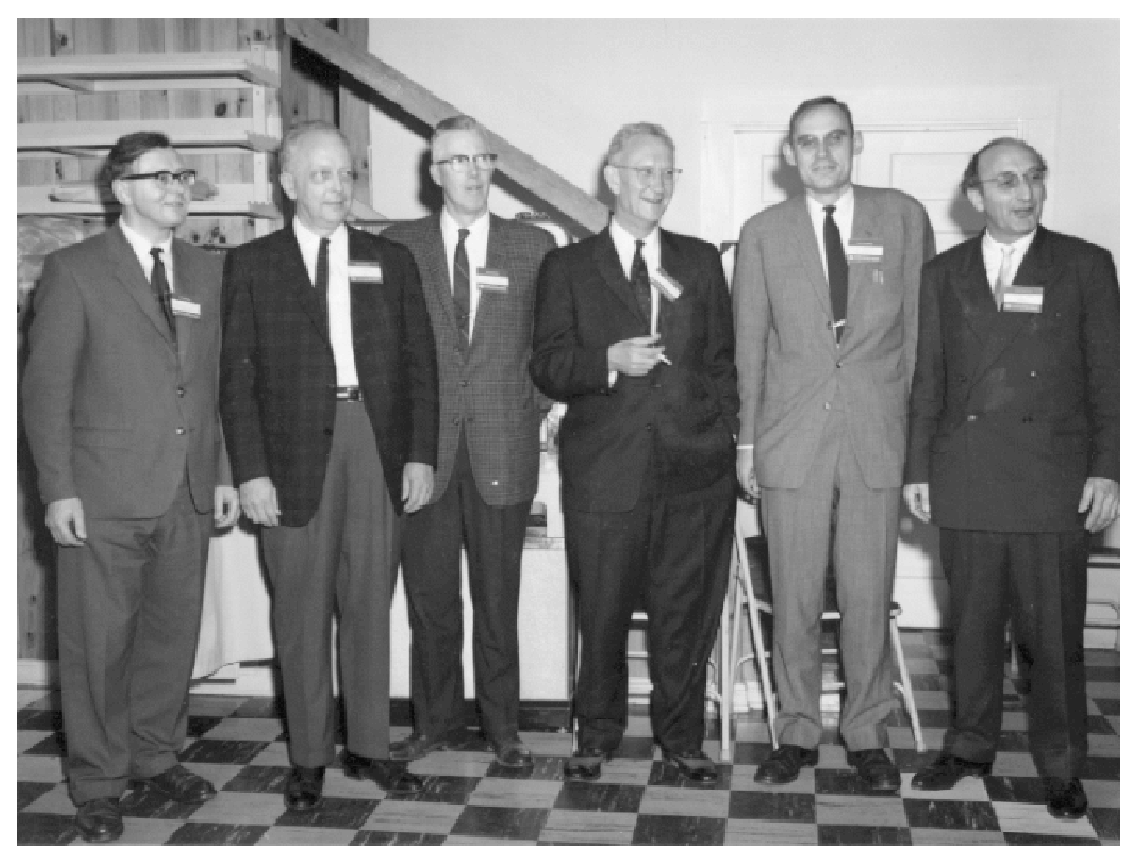
\includegraphics[width=0.41\linewidth]{Images/SVD/Image.originale.eps}}
\hspace{1cm}
\subfigure[Image obtenue par une troncature de la SVD à l'ordre 1]{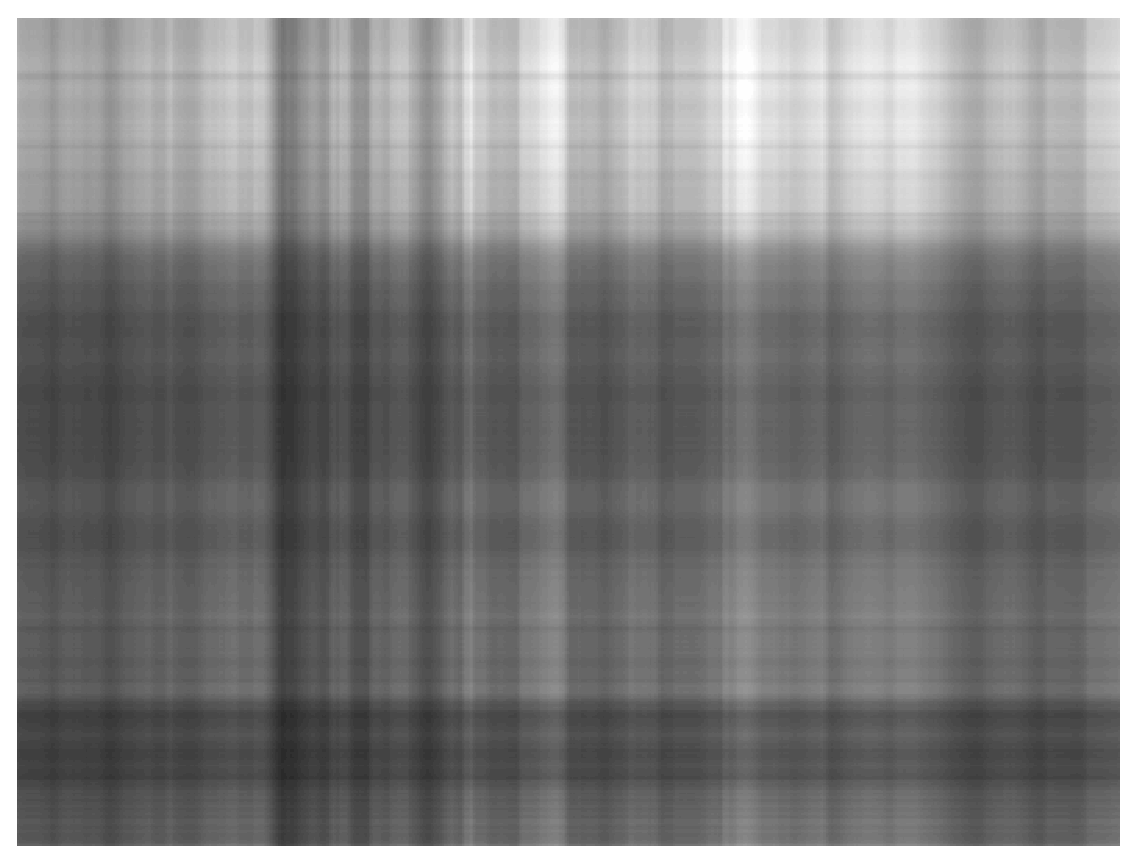
\includegraphics[width=0.41\linewidth]{Images/SVD/SVD.Tronquee.1.eps}}
\subfigure[à l'ordre 2]{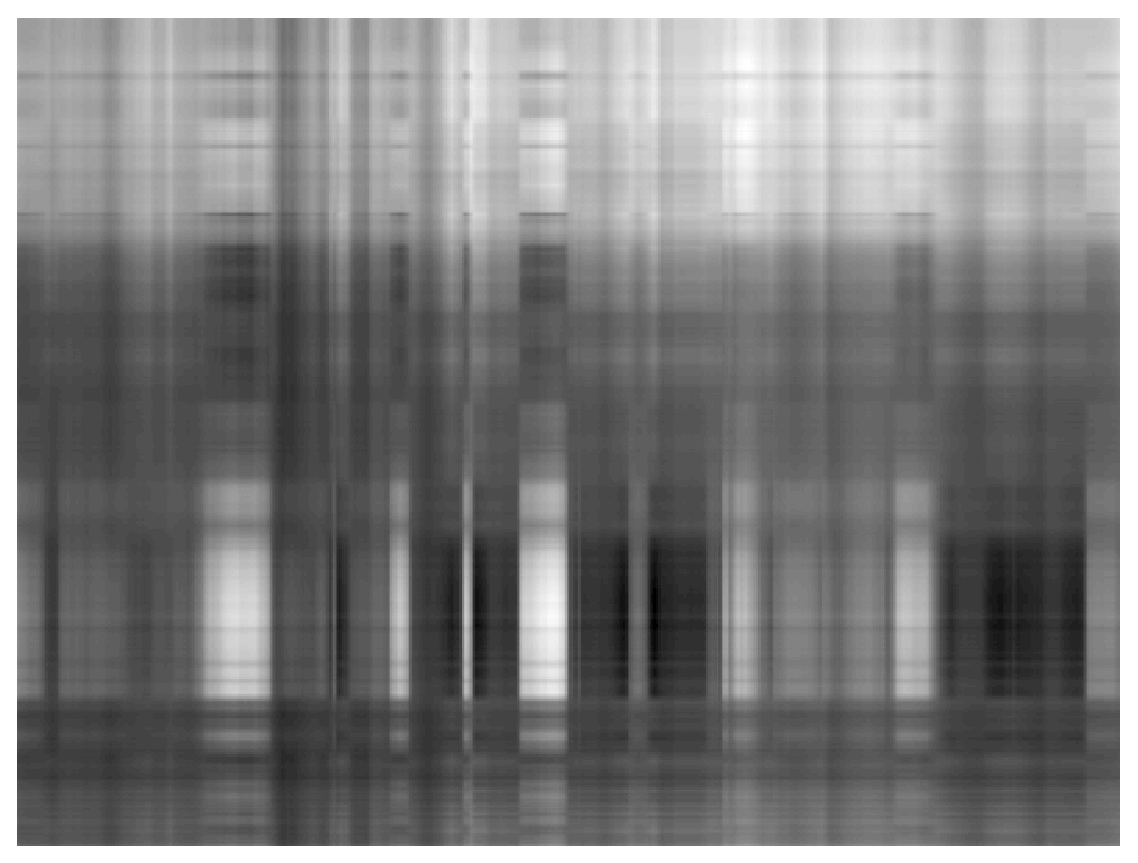
\includegraphics[width=0.41\linewidth]{Images/SVD/SVD.Tronquee.2.eps}}
\hspace{1cm}
\subfigure[à l'ordre 4]{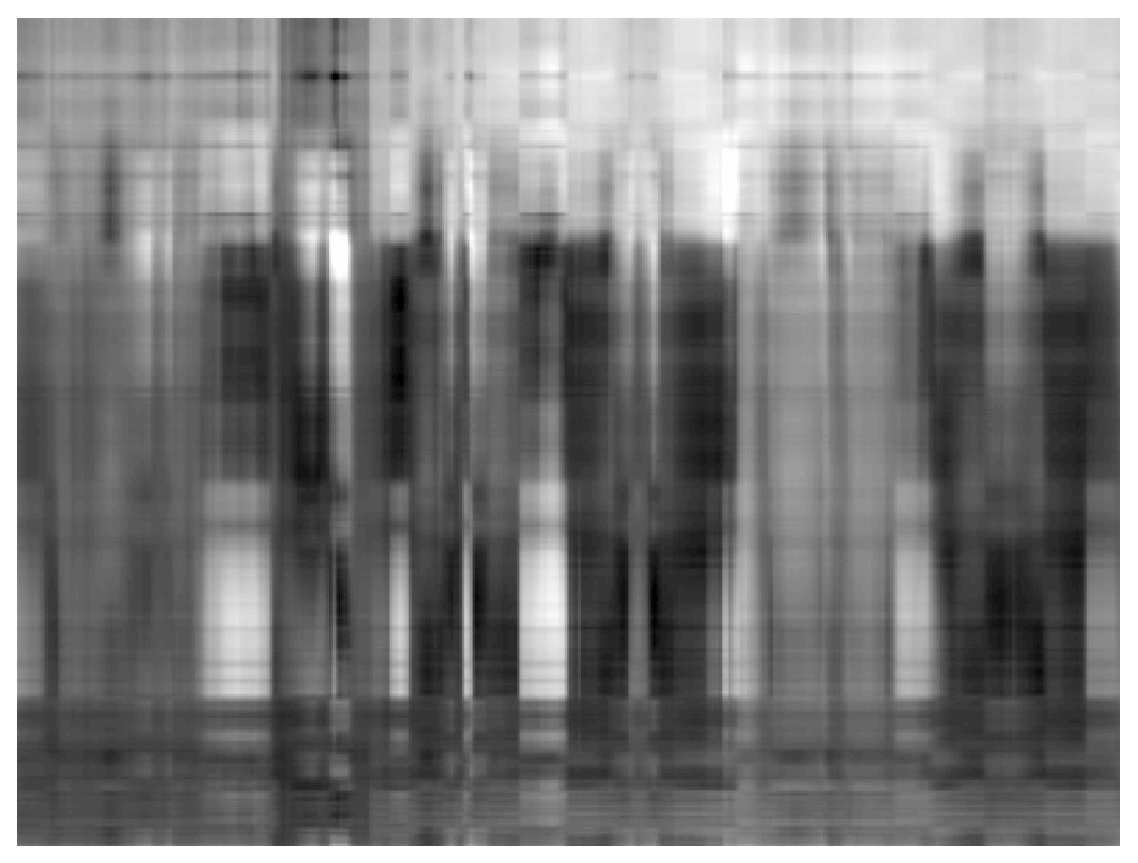
\includegraphics[width=0.41\linewidth]{Images/SVD/SVD.Tronquee.4.eps}}
\subfigure[à l'ordre 16]{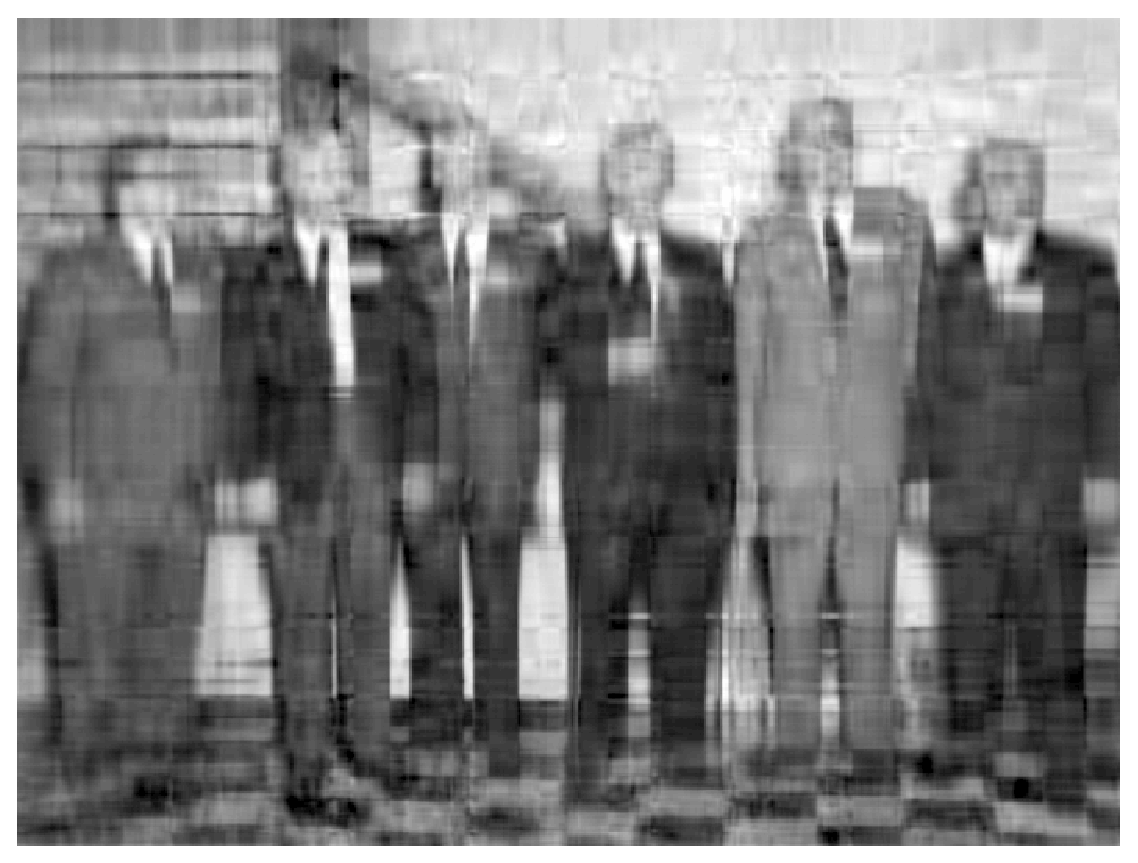
\includegraphics[width=0.41\linewidth]{Images/SVD/SVD.Tronquee.16.eps}}
\hspace{1cm}
\subfigure[à l'ordre 64]{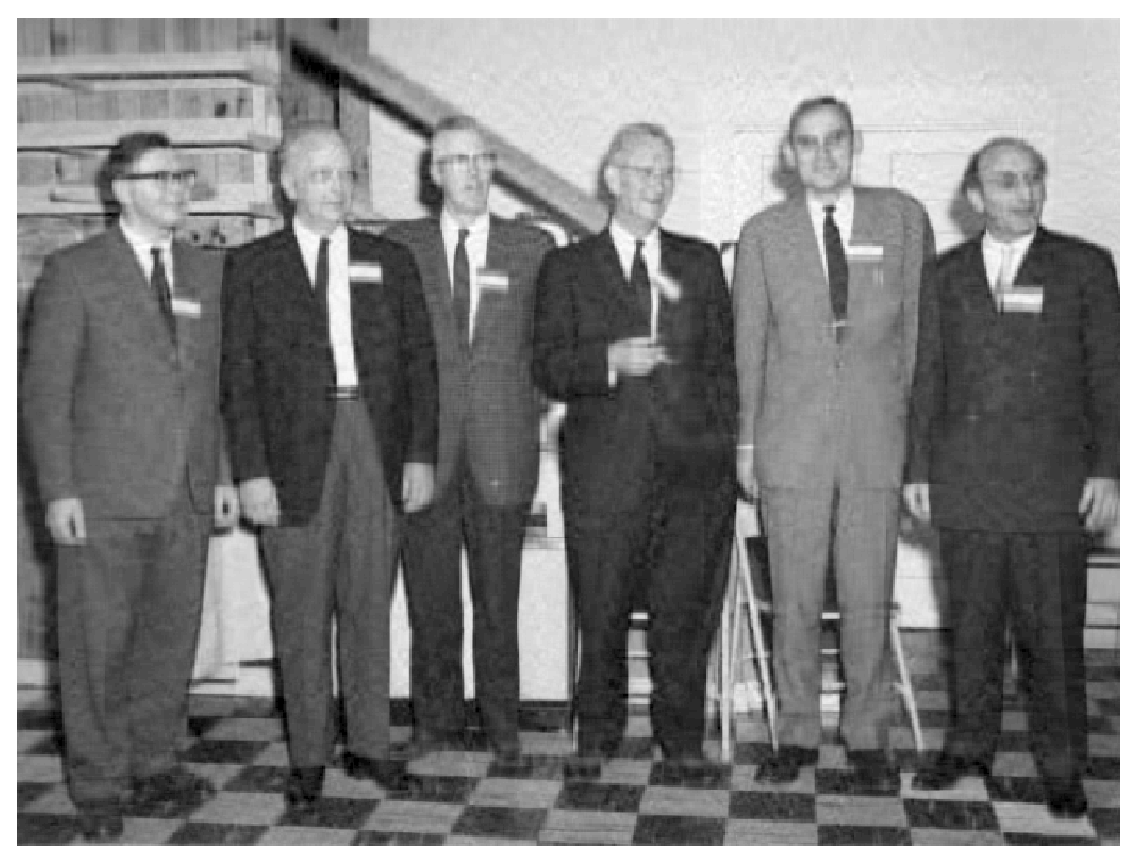
\includegraphics[width=0.41\linewidth]{Images/SVD/SVD.Tronquee.64.eps}}
\subfigure[à l'ordre 256]{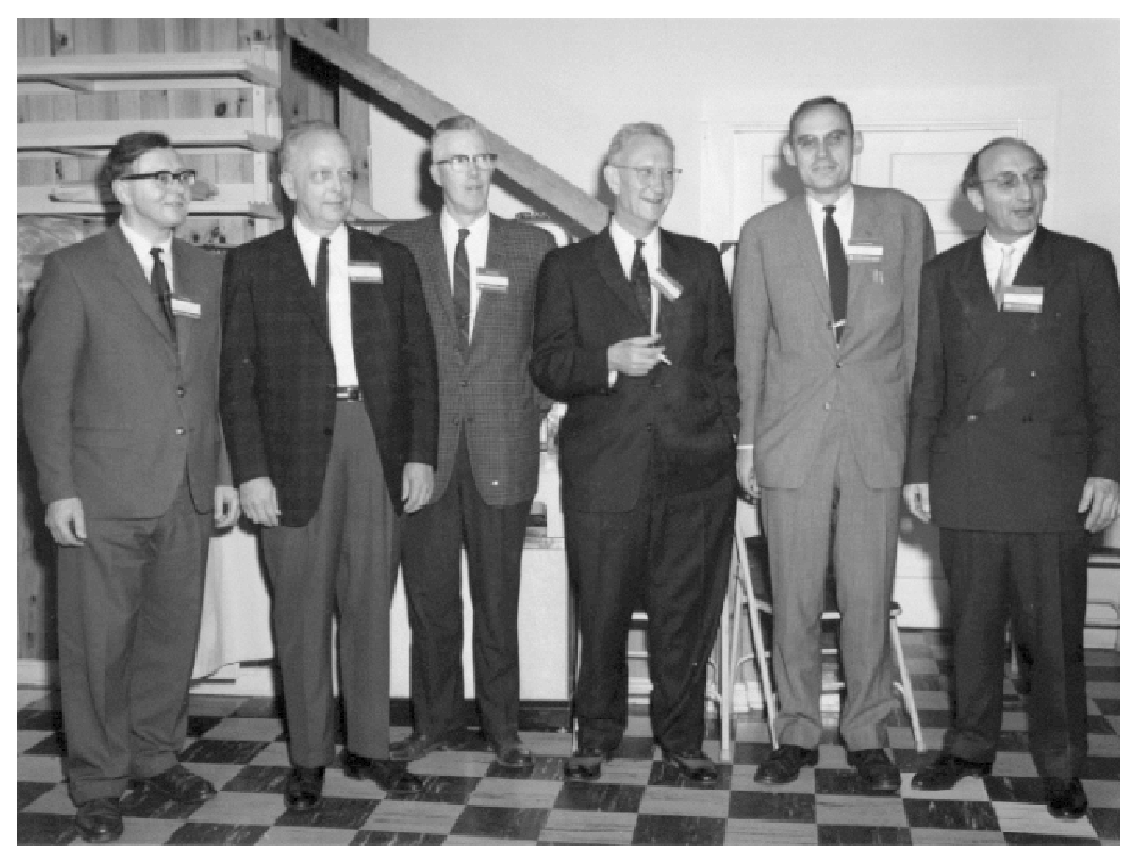
\includegraphics[width=0.41\linewidth]{Images/SVD/SVD.Tronquee.256.eps}}
\hspace{1cm}
\subfigure[Image obtenue par SVD sans troncature, rigouresement semblable à l'originale]{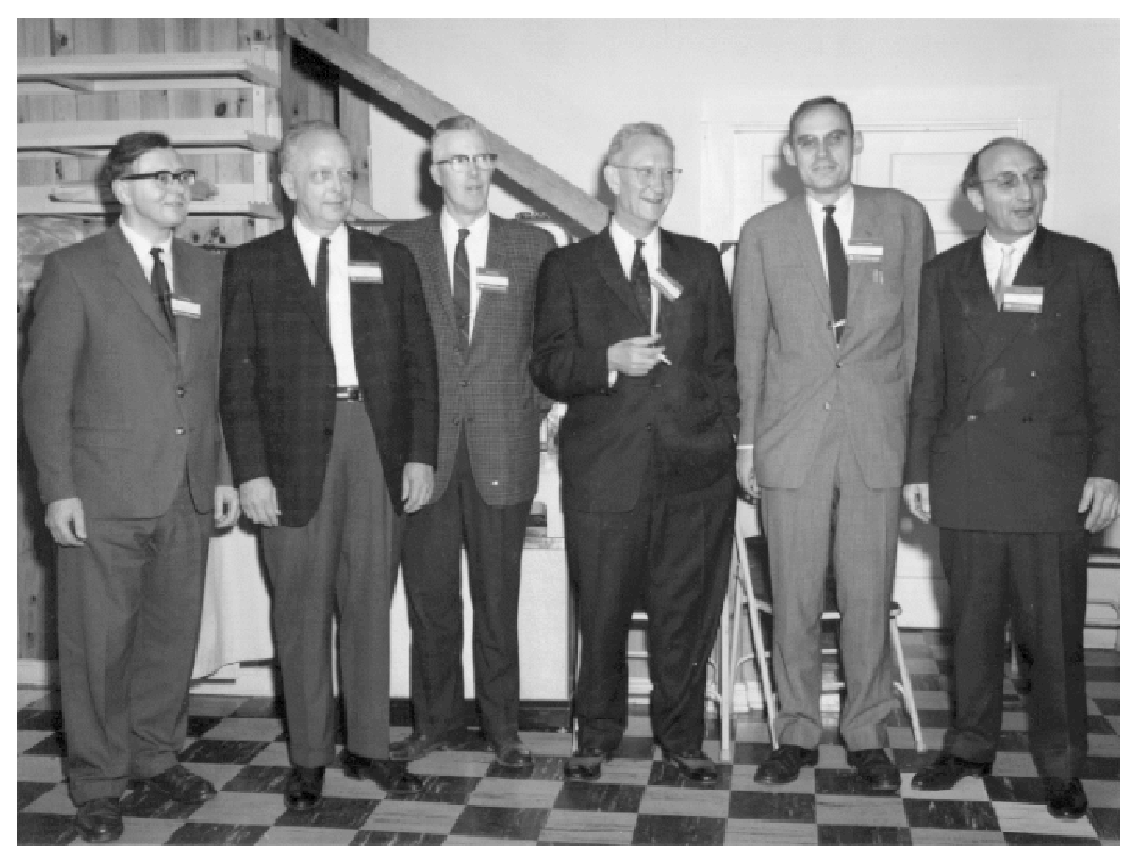
\includegraphics[width=0.41\linewidth]{Images/SVD/SVD.Total.eps}}
\caption{Compression d'une image par SVD}
\end{figure}

\clearpage

On constate donc que plus l'ordre de la troncature de la SVD est faible plus l'image obtenue est détériorée, et on peut voir dans le programme que le poids en est évidemment réduit. Ainsi l'image obtenue grâce à 256 modes ne semble pas distinguable de l'originale (mêmes sans le rétrécissement nécessaire pour l'afficher dans ce rapport), qui en compte 480, ceci permet donc de réaliser une compression des données jusqu'à une précision souhaitée
(note: Il existe des algorithmes plus performants que la SVD pour compresser les images). Voici la répartition des valeurs singulières de l'image (affichée avec un axe des ordonnées en semi-log pour être lisible étant donnée la disparité des valeurs): 

\begin{figure}[!ht]
\centering
\includegraphics[width=0.425\linewidth]{Images/SVD/Valeurs.Singulieres.Semilog.eps}
\caption{Valeurs singulières}
\end{figure}

\label{ValeursSing}
Évidemment plus les valeurs singulières décroissent rapidement, plus la troncature sera efficace. 

La SVD Tronquée assure l'optimalité de l'approximation car la matrice obtenue par une troncature à l'ordre $k$, est la matrice de rang $k$ qui minimise l'erreur : $  \Vert \mathbf{A} - \mathbf{A}^{(k)} \Vert_F$ . La norme de Frobenius est égale à la racine carrée de la somme des carrés de tous les termes d'une matrice (norme 2) et est aussi égale à plus grande valeur singulière. 

La SVD tronquée nécessite le calcule total de la SVD, ce qui représente un nombre d'opérations numériques de l'ordre de $O(mn^2)$ (qui est lié au temps de calcul). Et même si l'on peut choisir de transposer la matrice pour échanger le rôle de $m$ et $n$, cela représente un handicap qui s'amplifie en même temps que la taille de la matrice étudiée. Pour remédier à ceci des méthodes de décomposition approchées ont été développées, les méthodes LRMA (pour Low-Rank Matrix Approximation), et notamment la méthode QUIC-SVD, qui permet de maîtriser l'erreur causée par l'approximation \cite{QUIC-SVD}. 

La POD est le plus souvent utilisée en version discrète, car les bases de données le sont (par exemple due à l'échantillonnage expérimental), ou simplement à cause de la discrétisation utilisée par un solveur numérique. Une utilisation de la version continue se trouve dans \cite{Turbulence}, en voici la description.

\subsection{La formulation continue}
La POD est une méthode qui propose une solution à variables séparées sous la forme d'une somme de produits de fonctions. Prenons la fonction originale $z(x,t)$, elle sera approximée sous la forme :
\begin{equation}
\label{DecompoPOD}
z(x,t) \approx \sum_{k=1}^m a_k(t) \varphi_k(x)
\end{equation}

Dans la suite de ce rapport, $x$ désignera la coordonnée spatiale (donc est éventuellement un vecteur) et $t$ la coordonnée temporelle. La décomposition \ref{DecompoPOD} n'est pas unique car il faut choisir l'espace d'approximation contenant les $\varphi_k(x)$. Par exemple si $x$ est contenue dans un intervalle $\Omega$ de réel, alors les fonctions $\varphi_k(x)$ peuvent être choisies comme des séries de Fourier, des polynômes de Legendre, des polynômes de Tchebychev etc... Et ce choix influence évidemment le résultat obtenue pour les fonctions $a_k(t)$. On fait l'hypothèse que l'espace d'approximation des fonctions d'espace est bien choisi et que la somme tendra vers la solution $z(x,t)$ quand $m$ tend vers l'infini (plus précisément sur le domaine de définition de $z(x,t)$, hormis des éventuels ensembles de mesure nulle. Les lecteurs qui ne sont pas familiers avec la théorie des mesures peuvent consulter \cite{Analysis}. Ces considérations ne seront pas développées ici. Il en sera de même pour les questions d'intégrabilité des fonctions qui ne se posent pas en calcul discret. Si on choisit pour les fonctions $\varphi_k(x)$ une base orthonormée :
\begin{equation}
\int_\Omega \varphi_i(x) \varphi_j(x) dx = \delta_{ij}
\end{equation}

\noindent
On obtient la formule suivante pour $a_k(t)$ :
\begin{equation}
	a_k(t) = \int_\Omega z(x,t) \varphi_k(x) dx 
\end{equation}
alors la détermination de la fonction $a_k(t)$ ne dépend que de $\varphi_k(x)$.

Si la décomposition est optimale, i.e. si pour chaque terme de la somme, il n'existe pas de meilleure approximation, alors les termes sont appelés proper orthogonal nodes, et la somme proper orthogonal decomposition.

\noindent
Pour faire correspondre avec la formulation discrète on pose :
\begin{equation}
	\mathbf{A} 	= \mathbf{Q} \mathbf{V}^T 
				= \sum_{i=1}^m \mathbf{q_i} \mathbf{v_i}^T
		\text{ où } \mathbf{Q} = \mathbf{U}\mathbf{S}
\end{equation}

Dans cette forme discrète de l'équation \ref{DecompoPOD}, la matrice $\mathbf{A}$ représente $z(x,t)$ et les colonnes $\mathbf{q_i}$ représentent les fonctions $a_k(t)$. 
Le lien entre valeurs singulières et valeurs propres a été décrit précédemment, et ce rapprochement peut servir à la résolution du problème; On définit alors $\mathbf{B} = \mathbf{A}^T \mathbf{A}$, et on aura dans le cas continu en temps mais décrit de manière discrète sur l'espace:
\begin{equation}
	\text{B}_{ij} = \frac{1}{T} 
			\int_{t_0}^{t_0+T} z(x_i,t) z(x_j,t)dz
\end{equation}

Et si l'on passe à une formulation en dimension infinie, il y a une infinité de valeurs propres et B n'est plus une matrice mais une fonction de deux variables :
\begin{equation}
	B(x_1,x_2) = \frac{1}{T} 
			\int_{t_0}^{t_0+T} z(x_1,t) z(x_2,t)dz
\end{equation}
où $x_1$ et $x_2$ sont des variables continues définies sur $\Omega$. 

Soit $\boldsymbol{\psi}$ un vecteur propre de $\mathbf{B}$, de valeur propre associée $\lambda$, alors $\mathbf{B}\boldsymbol{\psi} = \lambda\boldsymbol{\psi}$. Ce qui s'écrit sous forme discrète :
\begin{equation}
\sum^m_{j=1} \text{B}_{ij} \psi_j^T = \lambda\psi_i
\end{equation}
ce qui devient une intégrale en forme continue :
\begin{equation}
\int_\Omega B(x_1,x_2) \psi(x_2) dx_2 = \lambda\psi(x_1 )
\end{equation}

Un des problèmes posés par cette réduction de modèles "a posteriori" est qu'elle dépend de la solution obtenue "a priori". En effet les modes trouvés sont représentatifs des données de départ, et si au cours d'un calcul la configuration du système considéré devait s'éloigner du résultat préalable, les modes ne seraient plus représentatifs de la solution. La représentation à variables séparées utilisée par la POD possède des limites, en particulier la mauvaise représentation d'une turbulence locale qui se déplace, typiquement : une onde de se propageant (la solution de l'équation de d'Alembert n'est pas à variable séparables : $f(x \pm \beta t )$.

\section{PGD}
Comme la POD, la PDG approxime la solution à l'aide de l'hypothèse de séparation des variables comme une somme de produits de fonctions; prenons la fonction solution $ z(x,t)$, elle sera approximée sous la forme :
\begin{equation}
z(x,t) \approx \sum^m_{k=1} a_k(t) \varphi_k(x)
\end{equation}

Mais à la différence de la POD, la fonction $z(x,t)$ est inconnue au préalable, on ne connaît alors pas les modes et on les calcule "à la volée", grâce à l'algorithme appelé algorithme des puissances itérées qui est le suivant :

%\begin{center}
%\begin{algorithm}
%\KwData{this text}
%\KwResult{how to write algorithm with \LaTeX2e }
%initialization\;
%\While{not at end of this document}{
%read current\;
%\eIf{understand}{
%go to next section\;
%current section becomes this one\;
%}{
%go back to the beginning of current section\;
%}
%}
%\caption{How to write algorithms}
%\end{algorithm}
%\end{center}

\begin{algorithm}
\caption{Résolution PGD}
\begin{algorithmic}[1]
\FOR{$m = 1 $ à $ m_{max}$}
\STATE initialiser $a_1$
\FOR{$k = 1 $ à $ k_{max}$}
\STATE $\varphi_k \leftarrow S_m(a_k )$
\STATE normer $\varphi_k$ ($\Vert\varphi_k\Vert_\Omega = 1$)
\STATE $a_k \leftarrow T_m (\varphi_k )$
\STATE vérifier la convergence de $(\varphi_k a_k)$
\ENDFOR
\STATE $\varphi_m \leftarrow \varphi_k$ et $a_m \leftarrow a_k$
\STATE $z_m = z_{m-1} + \varphi_m a_m$
\ENDFOR
\end{algorithmic}
\label{AlgoPGD}
\end{algorithm}
\label{AlgoPGDPartie}

%%%\REQUIRE $n \geq 0 \vee x \neq 0$
%%%\ENSURE $y = x^n$
%%\IF{$n < 0$}
%%\STATE $N \leftarrow -n$
%%\ELSE
%%\STATE $N \leftarrow n$
%%\ENDIF
%%\STATE $N \leftarrow N - 1$
%%\ENDFOR

Où $\text{S}_m$ est l'application qui associe à une fonction du temps $a$, une fonction de l'espace $\varphi$. Et $\text{T}_m$ l'application qui associe à une fonction spatiale $\varphi$, une fonction temporelle $a$. On part de la formulation faible d'un problème :
\begin{equation}
\label{ProblemeLM}
B(u,v) = L(v) ~~ \forall v \in H
\end{equation}

\label{LaxMilgram}
\noindent
Sous les hypothèses du théorème de Lax-Milgram :
\begin{itemize}
\item $H$ un espace de Hilbert
\item $B$ un forme bilinéaire, continue et coercive sur $H$
\item $L$ une forme linéaire continue sur $H$
\end{itemize}
il existe un unique u $\in$ H solution de l'équation \ref{ProblemeLM}.

On applique alors la démarche classique pour la PGD, appelée Galerkin progressive. On suppose $z_{m-1}$ (l'approximation de $z$ à l'ordre $m-1$) connue. Un nouveau couple $(\varphi, a) \in  U \otimes V$ est défini pour la décomposition d'ordre $m$ comme celui qui vérifie le critère de double orthogonalité de Galerkin suivant:
\begin{equation}
\label{formulationFaible}
B(z_{m-1} + \varphi a , \varphi a^* + \varphi^*  a) = L (\varphi a^* + \varphi^* a) ~~~
\forall \varphi^*  \in U \text{ et } \forall a^* \in V 
\end{equation}
Alors $S_m (a)$ est définie par :
\begin{equation}
B(z_{m-1} + \varphi a , \varphi^*  a) = L (\varphi^* a) ~~~
\forall \varphi^*  \in U
\end{equation}
et $T_m (\varphi)$ par :
\begin{equation}
B(z_{m-1} + \varphi a , \varphi a^*) = L (\varphi a^* ) ~~~
\forall a^* \in V 
\end{equation}

Le couple $(\varphi, a)$ vérifie l'équation \ref{formulationFaible} si et seulement si $\varphi = S_m (a)$ et $a = T_m (\varphi)$, qui est un problème non-linéaire, dont la résolution par la PGD peut être vue comme un problème aux valeurs propres où $\varphi$ et $a$ sont respectivement les fonctions propres dominantes de $S_m \circ T_m$ et $T_m \circ S_m$ . Ce qui permet en s'inspirant d'algorithmes utilisés dans les problèmes aux valeurs propres d'obtenir l'algorithme 1, qui donne la décomposition. Cet algorithme peut être modifié, notamment par l'ajout de l'orthogonalisation qui peut généralement améliorer les résultats (dans le cas ou il n'y a que deux variables). S'il on veut orthogonaliser $\varphi_m$ par rapport à la base spatial existante \{$\varphi_1 , \varphi_2 , ... , \varphi_{m-1}$\}, il faut définir un produit scalaire sur $\Omega$, par exemple : 
\begin{equation}
\langle u,v \rangle_\Omega = \int_\Omega \! uv ~ d\Omega
\end{equation}

Une autre modification consiste à introduire une fonction $T(\mathbf{p_m}) = \boldsymbol{\alpha}_\mathbf{m}$, où $\mathbf{p_m}$ est un vecteur qui contient les $\varphi_m$, et $\boldsymbol{\alpha}_\mathbf{m}$ un vecteur contenant les $a_m$. Permettant ainsi la mise à jour de l'ensemble des fonctions du temps après chaque calcul d'un nouveau couple $(\varphi_m , a_m )$, 
en remplaçant les lignes 9 et 10 de l'algorithme 1 par :

\begin{changemargin}{2cm}{0cm}
\begin{algorithmic}
\STATE $\varphi_m \leftarrow \varphi_k$
\STATE $\boldsymbol{\alpha}_\mathbf{m} \leftarrow T(p_m)$
\STATE $z_m = \mathbf{p_m} . \boldsymbol{\alpha}_\mathbf{m}$
\end{algorithmic}
\end{changemargin}

Pour voir un exemple d'utilisation de la méthode, \cite{Garanteed} propose une résolution d'un problème thermique avec la PGD. Le calcul pour un problème dynamique sera détailler dans une autre partie.


\chapter{Le calcul dynamique}

\noindent
L'équation de la dynamique \ref{PFD}, est valable à tout instant, rappel :
\[
\mathbf{M}\mathbf{\ddot{u}} + \mathbf{C}\mathbf{\dot{u}} + \mathbf{K}\mathbf{u} =
\mathbf{f}
\]

Il s'agit d'un équation différentielle en $\mathbf{u}$. Pour résoudre un équation différentielle il existe une méthode dite de résolution par quadrature. Cette méthode fournis une solution exacte et explicite pour l'équation, le problème est que cette résolution n'est possible que dans quelques cas classiques et elle est donc impossible dans le cas général. Dans ce cas on résout l'équation par une méthode numérique, cela induit la discrétisation de l'intervalle d'étude. En espace la discrétisation se traduit par le maillage, ce qui permet de définir les quantités dépendantes de l'espace comme des matrices. Le temps ne se représentant que sur une dimension, il suffit de choisir un pas de temps fixe pour découper le temps d'étude, et le représenter plus ou moins finement.

\section{Les schémas d'intégration}
\label{SchemasDIntegration}

Le fait de découper l'axe temporelle permet de résoudre l'équation à un instant donné (à condition de connaître la solution à l'instant précédent*). Pour ce faire il faut définir les liens entre les différentes dérivés de $\mathbf{u}$, on choisit alors un schéma d'intégration.

*Si un schéma n'utilise que la solution au pas de temps précédent et pas aux pas de temps antérieurs à celui-ci, on dit que ce schéma est à pas unique, sinon il est dit à pas multiples.

Pour décrire la dérivé d'une fonction discrète on peut utiliser les schémas d'Euler, de Runge-Kutta ou de Crank-Nicholson. Dans la cas particulier de la dynamique on utilise la méthode de Newmark qui définit les liens entre accélération, vitesse et déplacement. Ces liens sont définis dans deux équations comportant des paramètres qui peuvent rendre l'algorithme explicite ou implicite, et qui influencent sa stabilité.

Un schéma est dit stable si il contrôle l'accumulation d'erreur de calcul (arrondis). Certains schémas sont conditionnellement stables et la solution qu'il fournissent peut alors diverger. La condition de stabilité en dynamique et en générale une condition imposée à la discrétisation en temps : Choisir un pas de temps qui ne soit pas trop petit pour définir la propagation de l'information dans le maillage. La taille critique en dessous de laquelle le pas de temps ne doit pas se trouver est donc dépendante de la taille de maille.

\subsection{Schémas de Newmark}

\noindent
Le schéma d'intégration est donné par les deux équations :
\begin{equation}
\label{Newmark1}
	\mathbf{u_{n+1}} = \mathbf{u_n} + dt.\mathbf{\dot{u}_n}
	+ \frac{dt^2}{2}[(1-2\beta)\mathbf{\ddot{u}_n} + 2\beta\mathbf{\ddot{u}_{n+1}}]
\end{equation}
\begin{equation}
\label{Newmark2}
	\mathbf{\dot{u}_{n+1}} = \mathbf{\dot{u}_n} 
	+ dt[(1-\gamma)\mathbf{\ddot{u}_n} + \gamma \mathbf{\ddot{u}_{n+1}}]
\end{equation}

\noindent
La stabilité du schéma dépend des deux paramètre $\beta$ et $\gamma$ :
\begin{center}
\begin{tabular}{c c}
$\gamma \leq 1/2$
& Instable\\
$\gamma \geq 1/2 \text{ et } 2 \beta \leq \gamma$
&conditionnellement stable\\
$\gamma \geq 1/2 \text{ et } 2 \beta \geq \gamma$
&inconditionnellement stable\\
\end{tabular}
\end{center}

\noindent
Pour des valeurs particulières des paramètres on retrouve des méthodes classiques :
\begin{center}
\begin{tabular}{c c c c}
\textbf{Nom} & $\boldsymbol{\gamma}$ & $\boldsymbol{\beta}$ & \textbf{Propriétés}\\
\hline
Différences Centrées&1/2&0&explicite et conditionnellement stable\\
Fox Goodwin&1/2&1/12&conditionnellement stable\\
Accélération linéaire&1/2&1/6&conditionnellement stable\\
Accélération Moyenne&1/2&1/4&inconditionnellement stable\\
\end{tabular}
\end{center}

\noindent
L'équation de la dynamique peut être formulée ainsi :
\begin{equation}
	\mathbf{M} \mathbf{\ddot{u}} + \mathbf{C} \mathbf{\dot{u}} + \mathbf{K} \mathbf{u} = \mathbf{f}
\end{equation}

\noindent
Ce qui donne avec les equations \ref{Newmark1} et \ref{Newmark2}, si $\mathbf{K}$ ne dépend pas de $\mathbf{u}$:
\begingroup\small
\begin{equation}
	\overbrace{(\mathbf{M}+\mathbf{C} \gamma dt + \mathbf{K}\beta dt^2)}^{\mathbf{S}} \mathbf{\ddot{u}_{n+1}} 
	= \mathbf{f_{n+1}} 
	- \mathbf{C}\overbrace	{
						[\mathbf{\dot{u}_n} + dt (1-\gamma) \mathbf{\ddot{u}_n}]
					}
					^{\mathbf{\dot{u}^p_{n+1}}}
	-\mathbf{K}\overbrace	{
						[\mathbf{u_n} + dt \mathbf{\dot{u}_n} 
						 + \frac{dt^2}{2} (1-2\beta) \mathbf{\ddot{u}_n}]
					}
					^{\mathbf{u^p_{n+1}}}
\end{equation}
\endgroup

\noindent
Permettant de calculer en trois étapes, les valeurs de $\mathbf{\ddot{u}}$, $\mathbf{\dot{u}}$ et $\mathbf{u}$ :
\begin{equation}
	\left\{
		\begin{array}{r c l}
			\mathbf{\ddot{u}_{n+1}} 
			&=& \mathbf{S}^{-1} (  \mathbf{f_{n+1}} - \mathbf{C} \mathbf{\dot{u}^p_{n+1}} - \mathbf{K} \mathbf{u^p_{n+1}}  )
			\\
			\mathbf{\dot{u}_{n+1}} &=& \mathbf{\dot{u}^p_{n+1}} + dt \gamma \mathbf{\ddot{u}_{n+1}}
			\\
			\mathbf{u_{n+1}} &=& \mathbf{u^p_{n+1}} + dt^2 \beta \mathbf{\ddot{u}_{n+1}}
		\end{array}
	\right.
\end{equation}


\subsection{HHT}

La méthode HHT (ou HHT-$\alpha$) qui se base sur la méthode de Newmark, a été introduite dans \cite{HHT2} pour rajouter un paramètre $\alpha$ qui permet d'introduire un amortissement numérique.

\noindent
Le schéma d'intégration est toujours défini par \ref{Newmark1} et \ref{Newmark2}, mais il y a cette fois trois paramètres à choisir, que l'on peut réduire à un choix sur alpha uniquement, en suivant les conseils donnés par \cite{HHT2} :
%\begin{equation}
%	\mathbf{u_{n+1}} = \mathbf{u_n} + dt.\mathbf{\dot{u}_n}
%	+ \frac{dt^2}{2}[(1-2\beta)\mathbf{\ddot{u}_n} + 2\beta\mathbf{\ddot{u}_{n+1}}]
%\end{equation}
%\begin{equation}
%	\mathbf{\dot{u}_{n+1}} = \mathbf{\dot{u}_n} 
%	+ dt[(1-\gamma)\mathbf{\ddot{u}_n} + \gamma \mathbf{\ddot{u}_{n+1}}]
%\end{equation}
%avec :
\begin{equation}
	\left\{
		\begin{array}{r c l}
			\beta &=& ( 1- \alpha )^{2}/4
			\\
			\gamma &=& 1/2 - \alpha
			\\
			\alpha &\in& [-1/3;0]
		\end{array}
	\right.
\end{equation}

\noindent
L'équation de la dynamique donnée dans \cite{HHT} est formulée ainsi :
\begin{equation}
	\mathbf{M}{\mathbf{\ddot{u}_{n+1}}} 
	+ (1+\alpha)\mathbf{C}{\mathbf{\dot{u}_{n+1}}}
	- \alpha \mathbf{C}{\mathbf{\dot{u}_n}}
	+ (1+\alpha) \mathbf{K} \mathbf{u_{n+1}}
	- \alpha \mathbf{K} \mathbf{u_n}
	= (1+\alpha)\mathbf{f_{n+1}}  + \alpha \mathbf{f_n}
\end{equation}

\noindent
Ce qui donne, si $\mathbf{K}$ ne dépend pas de $\mathbf{u}$:

\begin{equation}
	\!\!\!\!\!\!\!
	\left\{
	\!\!\!\!\!\!\!\!
	\begin{array}{l l l}
		\begin{array}{r c l}
			& &\mathbf{M}{\mathbf{\ddot{u}_{n+1}}} 
			+ (1+\alpha)\mathbf{C} {\mathbf{\dot{u}_n}}
			+ (1+\alpha)\mathbf{C} dt (1-\gamma){\mathbf{\ddot{u}_n}}
			+ (1+\alpha)\mathbf{C} dt \gamma {\mathbf{\ddot{u}_{n+1}}} 
			- \alpha \mathbf{C} \mathbf{\dot{u}_n}
			\\
			&+& (1+\alpha)\mathbf{K} \mathbf{u_n}
			+ (1+\alpha)\mathbf{K} dt \mathbf{\dot{u}_n}
			+ (1+\alpha)\mathbf{K} \frac{dt^2}{2} (1-2 \beta){\mathbf{\ddot{u}_n}}
			+ (1+\alpha)\mathbf{K} \frac{dt^2}{2} 2 \beta {\mathbf{\ddot{u}_{n+1}}}
			- \alpha \mathbf{K} \mathbf{u_n}
			\\
			&=& (1+\alpha)\mathbf{f_{n+1}}  + \alpha \mathbf{f_n}
		\end{array}
		\\
		~~~$Soit, en factorisant les inconnues:$
		\\
		\begin{array}{r c l}
			   & &\overbrace{
			   			[\mathbf{M} + (1+ \alpha)(\mathbf{C} dt \gamma 
			   								+ \mathbf{K} dt^2 \beta)] }^{\mathbf{S_{H\!H\!T}} }
			   		\mathbf{\ddot{u}_{n+1}}
			\\ &+&(1+ \alpha)[\mathbf{C} dt (1- \gamma) + \mathbf{K} \frac{dt^2}{2} (1-2\beta)] 					\mathbf{\ddot{u}_n}
			\\ &+&[(1+ \alpha) (\mathbf{C} + \mathbf{K} dt)-\alpha \mathbf{C}] \mathbf{\dot{u}_n}
			\\ &+&[(1+ \alpha) \mathbf{K} -\alpha \mathbf{K}] \mathbf{u_n}
			
			\\ &=& (1+\alpha)\mathbf{f_{n+1}}  + \alpha \mathbf{f_n}
		\end{array}
		\\
		~~~$Soit, en factorisant les matrices:$
		\\
		\begin{array}{r c l}
			   & &\mathbf{S_{H\!H\!T} } \mathbf{\ddot{u}_{n+1}} 
			+\mathbf{C}\overbrace	{
						[\mathbf{\dot{u}_n} + (1+\alpha) dt (1-\gamma) \mathbf{\ddot{u}_n}]
					}
					^{\mathbf{\dot{u}_{n+1}^{\mathbf{p}H\!H\!T} }}			
			+\mathbf{K}\overbrace	{
						[\mathbf{u_n} + (1+ \alpha)( dt \mathbf{\dot{u}_n} 
						 + \frac{dt^2}{2} (1-2\beta) \mathbf{\ddot{u}_n})]
					}
					^{\mathbf{u_{n+1}^{pH\!H\!T} }}
			\\ &=& (1+\alpha)\mathbf{f_{n+1}}  - \alpha \mathbf{f_n}
		\end{array}
	\end{array}
	\right.
	\!\!\!\!\!\!\!\!\!\!\!\!\!\!\!\!\!\!\!\!\!\!
\end{equation}

\noindent
Permettant de calculer en trois étapes :
\begin{equation}
\label{Prediction}
	\left\{
		\begin{array}{r c l}
			\mathbf{\ddot{u}_{n+1}} 
			&=& \mathbf{ {S_{H\!H\!T}} }^{-1} (  \mathbf{f_{n+1}^{H\!H\!T} }
				- \mathbf{C} \mathbf{\dot{u}_{n+1}^{pH\!H\!T}} - \mathbf{K} \mathbf{u_{n+1}^{pH\!H\!T} } )
			\\ \mathbf{\dot{u}_{n+1}} &=& \mathbf{\dot{u}_n} 
				+ dt[(1-\gamma)\mathbf{\ddot{u}_n} + \gamma \mathbf{\ddot{u}_{n+1}}]
			\\ \mathbf{u_{n+1}} &=& \mathbf{u_n} + dt.\mathbf{\dot{u}_n}
				+ \frac{dt^2}{2}[(1-2\beta)\mathbf{\ddot{u}_n} + 2\beta\mathbf{\ddot{u}_{n+1}}]
		\end{array}
	\right.
\end{equation}
avec:
\begin{equation}
		\mathbf{f_{n+1}^{H\!H\!T}} = (1+\alpha)\mathbf{f_{n+1}}  - \alpha \mathbf{f_n}
\end{equation}

Si on ajoute un terme non-linéaire, on peut le représenter par l'ajout d'un élément au second membre f, ou recalculer la matrice $\mathbf{K}$.

\noindent
L'équation de la dynamique devient :

\begingroup\footnotesize
\begin{equation}
\label{RepresentationSecondMembre}
	\mathbf{M}{\mathbf{\ddot{u}_{n+1}}} 
	+ (1+\alpha)\mathbf{C}{\mathbf{\dot{u}_{n+1}}}
	- \alpha \mathbf{C}{\mathbf{\dot{u}_n}}
	+ (1+\alpha) \mathbf{K} \mathbf{u_{n+1}}
	- \alpha \mathbf{K} \mathbf{u_n}
	= (1+\alpha)\mathbf{f_{n+1}}  + \alpha \mathbf{f_n}
	- \underline{ ((1+\alpha) f_{(u_{n+1})} - \alpha f_{(u_n)}) }
\end{equation}
\endgroup
Ou :
\begin{equation}
\label{RepresentationKModifie}
	\mathbf{M}{\mathbf{\ddot{u}_{n+1}}} 
	+ (1+\alpha)\mathbf{C}{\mathbf{\dot{u}_{n+1}}}
	- \alpha \mathbf{C}{\mathbf{\dot{u}_n}}
	+ \underline{
	(1+\alpha) \mathbf{K}_{(u_{n+1})} \mathbf{u_{n+1}}
	- \alpha \mathbf{K}_{(u_{n})} \mathbf{u_n}  }
	= (1+\alpha)\mathbf{f_{n+1}}  + \alpha \mathbf{f_n}
\end{equation}


Si l'on choisit la représentation \ref{RepresentationSecondMembre} il suffit d'ajouter le terme souligné au second membre. Si l'on choisit la représentation \ref{RepresentationKModifie} les équations sont modifiées ainsi : 
\\ * Pour simplifier on notera $\mathbf{K} = \mathbf{K}_{(u_{n+1})}$ et on obtient des équations légèrement modifiées par les termes soulignés.


\begin{equation}
	\!\!\!\!\!\!\!
	\left\{
	\!\!\!\!\!\!\!\!
	\begin{array}{l l l}
		\begin{array}{r c l}
			& &\mathbf{M}{\mathbf{\ddot{u}_{n+1}}} 
			+ (1+\alpha)\mathbf{C} {\mathbf{\dot{u}_n}}
			+ (1+\alpha)\mathbf{C} dt (1-\gamma){\mathbf{\ddot{u}_n}}
			+ (1+\alpha)\mathbf{C} dt \gamma {\mathbf{\ddot{u}_{n+1}}} 
			- \alpha \mathbf{C} \mathbf{\dot{u}_n}
			\\
			&+& (1+\alpha)\mathbf{K} \mathbf{u_n}
			+ (1+\alpha)\mathbf{K} dt \mathbf{\dot{u}_n}
			+ (1+\alpha)\mathbf{K} \frac{dt^2}{2} (1-2 \beta){\mathbf{\ddot{u}_n}}
			+ (1+\alpha)\mathbf{K} \frac{dt^2}{2} 2 \beta {\mathbf{\ddot{u}_{n+1}}}
			- \underline{\alpha \mathbf{K}_{(u_{n})} \mathbf{u_n} }
			\\
			&=& (1+\alpha)\mathbf{f_{n+1}}  + \alpha \mathbf{f_n}
		\end{array}
		\\
		~~~$Soit, en factorisant les inconnues:$
		\\
		\begin{array}{r c l}
			   & &\overbrace{
			   			[\mathbf{M} + (1+ \alpha)(\mathbf{C} dt \gamma 
			   								+ \mathbf{K} dt^2 \beta)] }^{\mathbf{S_{H\!H\!T}} }
			   		\mathbf{\ddot{u}_{n+1}}
			\\ &+&(1+ \alpha)[\mathbf{C} dt (1- \gamma) + \mathbf{K} \frac{dt^2}{2} (1-2\beta)] 					\mathbf{\ddot{u}_n}
			\\ &+&[(1+ \alpha) (\mathbf{C} + \mathbf{K} dt)-\alpha \mathbf{C}] \mathbf{\dot{u}_n}
			\\ &+&[(1+ \alpha) \mathbf{K} 
				-\underline{\alpha \mathbf{K}_{(u_{n})}}] \mathbf{u_n}
			
			\\ &=& (1+\alpha)\mathbf{f_{n+1}}  + \alpha \mathbf{f_n} 
		\end{array}
		\\
		~~~$Soit, en factorisant les matrices:$
		\\
		\begin{array}{r c l}
			   & & \mathbf{S_{H\!H\!T}} \mathbf{\ddot{u}_{n+1}} 
			+\mathbf{C}\overbrace	{
						[\mathbf{\dot{u}_n} + (1+\alpha) dt (1-\gamma) \mathbf{\ddot{u}_n}]
					}
					^{\mathbf{\dot{u}_{n+1}^{pH\!H\!T} }}			
			+\mathbf{K}\overbrace	{
						[u_n + (1+ \alpha)( dt \mathbf{\dot{u}_n} 
						 + \frac{dt^2}{2} (1-2\beta) \mathbf{\ddot{u}_n})]
					}
					^{\mathbf{u_{n+1}^{pH\!H\!T}} }
			\\ &=& (1+\alpha)\mathbf{f_{n+1}}  - \alpha \mathbf{f_n}
			    - \underline{ \alpha (\mathbf{K}-\mathbf{K}_{(u_{n})} ) \mathbf{u_n}}
		\end{array}
	\end{array}
	\right.
	\!\!\!\!\!\!\!\!\!\!\!\!\!\!\!\!\!\!\!\!\!
	\!\!\!\!\!\!\!\!\!\!\!\!\!\!\!\!\!\!\!\!\!
\end{equation}

\noindent
Et on retrouve les équations \ref{Prediction} mais cette fois :
\begin{equation}
		\mathbf{f_{n+1}^{H\!H\!T}} = (1+\alpha)\mathbf{f_{n+1}}  
		- \alpha \mathbf{f_n} - \underline{ \alpha (\mathbf{K}-\mathbf{K}_{(u_{n})} ) \mathbf{u_n}}
\end{equation}

\section{La PGD} 


\subsection{Définition du problème}

\begin{itemize}
\item Admissibilité cinématique :
	\\$U \in [H^1(\Omega)]^3, U_{|\partial \Omega_U} = U_d $
\item Admissibilité statique :
	\\$ div \sigma + f_v = \rho \ddot{U} + \mu \dot{U}$ sur $\Omega$ 
		et $\sigma . n _{|\partial \Omega_f} = f_d$
\item Relation de comportement :
	\\$\sigma = H : \varepsilon (U)$ sur $ \Omega$
\item Conditions initiales :
	\\$U(0) = U_0$ et $ \dot{U}(0) = \dot{U}_0$
\end{itemize}

\noindent
Formulation variationnelle : 
\begin{equation}
	\forall U^* ~ \text{CA0,} ~
		\int_\Omega [\varepsilon (U^*) : \sigma   
					+ U^* \mu \dot{U} 
					+ U^* \rho \ddot{U}
					- U^* f_d
					] d \Omega	
		- \int_{\partial \Omega_f} U^* f_d  ds		
		- \underbrace{
			\int_{\partial \Omega_U} U^* \sigma . n ds	
		  }_{=0}
		= 0
\end{equation}

\noindent
Où
\begin{itemize}
\item $U$ est le déplacement
\item $\Omega$ l'espace, avec le bord $\partial \Omega = \partial \Omega_U \cap \partial \Omega_f$
\item $\sigma$ le tenseur des contraintes
\item $\varepsilon$ le tenseur des déformations
\item $\rho$ la masse volumique
\item $\mu$ l'amortissement volumique (cette donnée est généralement mal connue)
\item $H$ le tenseur de Hook
\item $f_v$ effort volumique
\item $f_d$ effort imposé sur $\partial \Omega_f$
\end{itemize}
\vspace{0.3cm}

\noindent
Mise en place de la PGD, utilisation de l'hypothèse des variables séparables :
\begin{equation}
	U(x,t,\theta) = \sum_{k=1}^n \varphi_k(x) g_k(t)h_k(\theta)
\end{equation}

\noindent
Où
\begin{itemize}
\item $x$ est la variable d'espace
\item $t$ la variable de temps
\item $\theta$ une variable paramètre utilisée à titre d'exemple
\end{itemize}
\vspace{0.3cm}

Pour chaque $k$, il faut discrétiser les fonctions sur leur domaine de définition, ici la discrétisation en espace donne : 
\begin{equation}
	\begin{array}{l c l c l}
		\varphi(x) &=& \sum_{i=1}^{Nbc_x}  N_i (x) \varphi_i &=& N_\varphi(x) \boldsymbol{\varphi_q} \\
	\end{array}
\end{equation}

$Nbc_x$ représente le nombre de composante de discrétisation spatiale, l'indice $q$ représente le vecteur sur le domaine discrétisé.

On remplace dans la formulation variationnelle, en choisissant $U^* = (\varphi gh)^* = ( \varphi^*gh+\varphi g^*h+\varphi gh^*) $.

\noindent
On rassemble les termes en $N_\varphi(x)$ ce qui permet de définir :
\begin{equation}
\mathbf{K} = \int_\Omega \varepsilon (N_\varphi(x)) : H : \varepsilon (N_\varphi(x))~~dx
\end{equation}
\begin{equation}
\mathbf{C} = \int_\Omega N_\varphi(x) \mu  N_\varphi(x)~~dx
\end{equation}
\begin{equation}
\mathbf{M} = \int_\Omega N_\varphi(x) \rho  N_\varphi(x)~~dx
\end{equation}
\begin{equation}
\mathbf{f} = \int_\Omega N_\varphi(x) f_v ~~dx 
	%+ \int_{\partial \Omega_U} U_d (H : \varepsilon (N_\varphi(x)) . n) 
	+ \int_{\partial \Omega_f} N_\varphi(x) f_d ~ds dt d\theta
\end{equation}

\noindent
Les calculs sont déroulés en annexes et donnent :
\begin{equation}
\!\!\!\!\!\!\!\!\!\!\!\!\!\!\!\!\!\!\!\!\!\!\!\!\!\!\!\!\!\!\!\!\!\!\!\!\!\!\!\!\!\!\!\!\!\!\!
\begin{array}{l}
	\displaystyle	
	\int_T \! \int_\Theta	\!\!
		\big(\boldsymbol{\varphi_q}^*gh + \boldsymbol{\varphi_q}g^*h + \boldsymbol{\varphi_q}gh^*\big)^T \!
					\bigg[~\mathbf{K}~ \boldsymbol{\varphi_q}gh
						+ ~\mathbf{C}~ \boldsymbol{\varphi_q} \dot{g}h 
						+ ~\mathbf{M}~ \boldsymbol{\varphi_q} \ddot{g}h
	\\ 
	  \displaystyle
		\phantom{\int_T\int_\Theta\big(\boldsymbol{\varphi_q}^{*T}gh + \boldsymbol{\varphi_q}g^*h + \boldsymbol{\varphi_q}gh^*}
			+ \mathbf{K} \sum_{k=1}^{n-1} (\boldsymbol{\varphi_q})_k       g_k  h_k 
			+ \mathbf{C} \sum_{k=1}^{n-1} (\boldsymbol{\varphi_q})_k  \dot{g_k} h_k 
			+ \mathbf{M} \sum_{k=1}^{n-1} (\boldsymbol{\varphi_q})_k \ddot{g_k} h_k
	\\ \displaystyle
	  
		\phantom{\int_T\int_\Theta\big(\boldsymbol{\varphi_q}^{*T}gh + \boldsymbol{\varphi_q}g^*h + \boldsymbol{\varphi_q}gh^*} -\mathbf{f}~\bigg] ~dt d\theta
	= 0
\end{array}
\!\!\!\!\!\!\!\!\!\!\!\!\!\!\!\!\!\!\!\!\!\!\!
\end{equation}
Ce qui permet de dégager un problème à résoudre pour chaque variable.


\subsection{Problème en espace}
\label{ProbEspace}
\begin{equation}
\!\!\!\!
\begin{array}{r r l}
	\forall \boldsymbol{\varphi_q}^*
	&\int_T \! \int_\Theta \!\!\!&		
		\boldsymbol{\varphi_q}^{*T}gh [~\mathbf{K}~ \boldsymbol{\varphi_q}gh
						+ ~\mathbf{C}~ \boldsymbol{\varphi_q} \dot{g}h 
						+ ~\mathbf{M}~ \boldsymbol{\varphi_q} \ddot{g}h
	\\
	  &&
		\phantom{\boldsymbol{\varphi_q}^{*T}gh
			}+ \mathbf{K}~ \sum_{k=1}^{n-1} (\boldsymbol{\varphi_q})_k       g_k  h_k 
			+  \mathbf{C}~ \sum_{k=1}^{n-1} (\boldsymbol{\varphi_q})_k  \dot{g_k} h_k 
			+  \mathbf{M}~ \sum_{k=1}^{n-1} (\boldsymbol{\varphi_q})_k \ddot{g_k} h_k
	\\
	  &&
		\phantom{\boldsymbol{\varphi_q}^{*T}gh} -\mathbf{f}~] ~dt d\theta ~~= 0
\end{array}
\end{equation}

\noindent
Donc:
\begin{equation}
\begin{array}{r l}
	\int_T \! \int_\Theta &		
		gh [~\mathbf{K}~ \boldsymbol{\varphi_q}gh
						+ ~\mathbf{C}~ \boldsymbol{\varphi_q} \dot{g}h 
						+ ~\mathbf{M}~ \boldsymbol{\varphi_q} \ddot{g}h
	\\
	  &
		\phantom{gh
			}+ \mathbf{K}~ \sum_{k=1}^{n-1} (\boldsymbol{\varphi_q})_k       g_k  h_k 
			+  \mathbf{C}~ \sum_{k=1}^{n-1} (\boldsymbol{\varphi_q})_k  \dot{g_k} h_k 
			+  \mathbf{M}~ \sum_{k=1}^{n-1} (\boldsymbol{\varphi_q})_k \ddot{g_k} h_k
	\\
	  &
		\phantom{\boldsymbol{\varphi_q}^{*T}gh} -\mathbf{f}~] ~dt d\theta ~~= 0
\end{array}
\end{equation}

\noindent
Soit:
\begin{equation}
\begin{array}{r r l}
	&& \displaystyle
		\int_T \! \int_\Theta
			gh [  ~\mathbf{K}~ gh
				+ ~\mathbf{C}~ \dot{g}h 
				+ ~\mathbf{M}~ \ddot{g}h
				] ~dt d\theta 
	~ \boldsymbol{\varphi_q}
	\\
	= &-& \displaystyle
		\int_T \! \int_\Theta		
			gh [  \mathbf{K} \sum_{k=1}^{n-1} (\boldsymbol{\varphi_q})_k       g_k  h_k 
				+ ~\mathbf{C} \sum_{k=1}^{n-1} (\boldsymbol{\varphi_q})_k  \dot{g_k} h_k 
				+ ~\mathbf{M} \sum_{k=1}^{n-1} (\boldsymbol{\varphi_q})_k \ddot{g_k} h_k
				- ~\mathbf{f}] ~dt d\theta				
\end{array}
\end{equation}
Système auquel il faut rajouter les conditions limites en déplacement $U_d$ par une méthode quelconque : substitution, multiplicateur de Lagrange... Dans le deuxième cas on change :

\begin{equation}
~\mathbf{M}=
	\begin{bmatrix}
	   \mathbf{M} & 0 \\
	   0 & 0 \\
	\end{bmatrix}
	\textrm{,  }
	\mathbf{C}=
	\begin{bmatrix}
	   \mathbf{C} & 0 \\
	   0 & 0 \\
	\end{bmatrix}
	\textrm{,  } 
	\mathbf{K}=
	\begin{bmatrix}
	   \mathbf{K} & \mathbf{D}^T \\
	   \mathbf{D} & 0 \\
	\end{bmatrix}
	\textrm{,  }
	\boldsymbol{\varphi_q}=
	\begin{bmatrix}
	   \boldsymbol{\varphi_q} \\
	   \boldsymbol{\lambda}\\
	\end{bmatrix}
	\textrm{ et }
	\mathbf{f}=
	\begin{bmatrix}
	   \mathbf{f} \\
	   \mathbf{b} \\
	\end{bmatrix}
\end{equation}
Où $\mathbf{D}$ et $\mathbf{b}$ représentent les déplacement imposés de la manière suivante:
$\mathbf{D} \boldsymbol{\varphi_q}= \mathbf{b}$.

\subsection{Problème en temps}
\begin{equation}
\begin{array}{r r l}
	\forall g^*
	&\int_T \! \int_\Theta \!\!\!&		
		\boldsymbol{\varphi_q}^Tg^*h [~\mathbf{K}~ \boldsymbol{\varphi_q}gh
						+ ~\mathbf{C}~ \boldsymbol{\varphi_q} \dot{g}h 
						+ ~\mathbf{M}~ \boldsymbol{\varphi_q} \ddot{g}h
	\\
	  &&
		\phantom{\boldsymbol{\varphi_q}g^*h
			}+ \mathbf{K}~ \sum_{k=1}^{n-1} (\boldsymbol{\varphi_q})_k       g_k  h_k 
			+  \mathbf{C}~ \sum_{k=1}^{n-1} (\boldsymbol{\varphi_q})_k  \dot{g_k} h_k 
			+  \mathbf{M}~ \sum_{k=1}^{n-1} (\boldsymbol{\varphi_q})_k \ddot{g_k} h_k
	\\
	  &&
		\phantom{\boldsymbol{\varphi_q}^{*T}gh} -\mathbf{f}~] ~dt d\theta ~~=0
\end{array}
\end{equation}

Donc:
\begin{equation}
\begin{array}{r l}
	\int_\Theta&		
		\boldsymbol{\varphi_q}^Th [    ~\mathbf{K}~ \boldsymbol{\varphi_q}gh
				+ ~\mathbf{C}~ \boldsymbol{\varphi_q}  \dot{g}h 
				+ ~\mathbf{M}~ \boldsymbol{\varphi_q} \ddot{g}h 
	\\
	  &
		\phantom{\boldsymbol{\varphi_q}h
			}+ \mathbf{K}~ \sum_{k=1}^{n-1} (\boldsymbol{\varphi_q})_k       g_k  h_k 
			+ ~\mathbf{C}~ \sum_{k=1}^{n-1} (\boldsymbol{\varphi_q})_k  \dot{g_k} h_k 
			+ ~\mathbf{M}~ \sum_{k=1}^{n-1} (\boldsymbol{\varphi_q})_k \ddot{g_k} h_k
	\\
	  &
		\phantom{\boldsymbol{\varphi_q}^{*T}h} -\mathbf{f}~] ~d\theta ~~=0
\end{array}
\end{equation}

Soit:
\begin{equation}
\begin{array}{r r l}
	&& \displaystyle
		\int_\Theta		
			\boldsymbol{\varphi_q}^Th [    ~\mathbf{K}~ \boldsymbol{\varphi_q}h ] ~d\theta
	~g
	+ 
		\int_\Theta		
			\boldsymbol{\varphi_q}^Th [ ~\mathbf{C}~ \boldsymbol{\varphi_q}h ] ~d\theta
	  ~\dot{g}
	+ 
		\int_\Theta		
			\boldsymbol{\varphi_q}^Th [ ~\mathbf{M}~ \boldsymbol{\varphi_q}h ] ~d\theta
	  ~\ddot{g}
	\\
	= &-& \displaystyle
		\int_\Theta		
			\boldsymbol{\varphi_q}^Th [  \mathbf{K}~ \sum_{k=1}^{n-1} (\boldsymbol{\varphi_q})_k       g_k  h_k 
				+ ~\mathbf{C}~ \sum_{k=1}^{n-1} (\boldsymbol{\varphi_q})_k  \dot{g_k} h_k 
				+ ~\mathbf{M}~ \sum_{k=1}^{n-1} (\boldsymbol{\varphi_q})_k \ddot{g_k} h_k
				- ~\mathbf{f}~ ] ~d\theta
\end{array}
\end{equation}

On se trouve donc en présence d'une équation différentielle en $g$, que l'on peut résoudre comme on résout classiquement un problème de dynamique, i.e. en utilisant un schéma d'intégration comme il en est question dans la section précédente. On peut aussi choisir résoudre en utilisant des élément finis temporels, le calcul est fournis en annexes.

\subsection{Problème en paramètre}
\begin{equation}
\begin{array}{r r l}
	\forall h^*
	&\int_T \! \int_\Theta \!\!\!&		
		\boldsymbol{\varphi_q}^Tgh^* [~\mathbf{K}~ \boldsymbol{\varphi_q}gh
						+ ~\mathbf{C}~ \boldsymbol{\varphi_q} \dot{g}h 
						+ ~\mathbf{M}~ \boldsymbol{\varphi_q} \ddot{g}h
	\\
	  &&
		\phantom{\boldsymbol{\varphi_q}g^*h
			}+ \mathbf{K}~ \sum_{k=1}^{n-1} (\boldsymbol{\varphi_q})_k       g_k  h_k 
			+ ~\mathbf{C}~ \sum_{k=1}^{n-1} (\boldsymbol{\varphi_q})_k  \dot{g_k} h_k 
			+ ~\mathbf{M}~ \sum_{k=1}^{n-1} (\boldsymbol{\varphi_q})_k \ddot{g_k} h_k
	\\
	  &&
		\phantom{\boldsymbol{\varphi_q}^{*T}gh} -\mathbf{f}~] ~dt d\theta ~~=0
\end{array}
\end{equation}

Donc:
\begin{equation}
\begin{array}{r l}
	\int_T &		
		\boldsymbol{\varphi_q}^Tg [~\mathbf{K}~ \boldsymbol{\varphi_q}gh
						+ ~\mathbf{C}~ \boldsymbol{\varphi_q} \dot{g}h 
						+ ~\mathbf{M}~ \boldsymbol{\varphi_q} \ddot{g}h
	\\
	  &
		\phantom{\boldsymbol{\varphi_q}h
			}+ \mathbf{K}~ \sum_{k=1}^{n-1} (\boldsymbol{\varphi_q})_k       g_k  h_k 
			+ ~\mathbf{C}~ \sum_{k=1}^{n-1} (\boldsymbol{\varphi_q})_k  \dot{g_k} h_k 
			+ ~\mathbf{M}~ \sum_{k=1}^{n-1} (\boldsymbol{\varphi_q})_k \ddot{g_k} h_k
	\\
	  &
		\phantom{\boldsymbol{\varphi_q}^{*T}gh} -\mathbf{f}~] ~dt ~~=0
\end{array}
\end{equation}

Soit:
\begin{equation}
\begin{array}{r r l}
	&& \displaystyle
		\int_T
			\boldsymbol{\varphi_q}^Tg [  ~\mathbf{K}~ \boldsymbol{\varphi_q} g
				+ ~\mathbf{C}~ \boldsymbol{\varphi_q} \dot{g}
				+ ~\mathbf{M}~ \boldsymbol{\varphi_q} \ddot{g}
				] ~dt
	~ h
	\\
	= &-& \displaystyle
		\int_T
			\boldsymbol{\varphi_q}^Tg [  \mathbf{K}~ \sum_{k=1}^{n-1} (\boldsymbol{\varphi_q})_k       g_k  h_k 
				+ ~\mathbf{C}~ \sum_{k=1}^{n-1} (\boldsymbol{\varphi_q})_k  \dot{g_k} h_k 
				+ ~\mathbf{M}~ \sum_{k=1}^{n-1} (\boldsymbol{\varphi_q})_k \ddot{g_k} h_k
				- ~\mathbf{f}~] ~dt
\end{array}
\end{equation}
\newpage



\chapter{Programmation}


\section{Plan du programme}

\begin{figure}[ht!]

\begin{center}
\scalebox{0.9} % Change this value to rescale the drawing.
{
\begin{pspicture}(0,-7.9)(8.8,7.9)
\definecolor{color1098b}{rgb}{0.8,0.8,1.0}
\definecolor{color1042b}{rgb}{0.8,1.0,0.8}
\psframe[linewidth=0.04,framearc=0.5,dimen=outer,fillstyle=solid,fillcolor=color1098b](5.0,5.1)(0.4,3.3)
\psframe[linewidth=0.04,framearc=0.5,dimen=outer,fillstyle=solid,fillcolor=color1098b](5.0,2.3)(0.4,0.5)
\psframe[linewidth=0.04,framearc=0.5,dimen=outer,fillstyle=solid,fillcolor=color1098b](5.0,-0.5)(0.4,-2.3)
\psframe[linewidth=0.04,framearc=0.5,dimen=outer,fillstyle=solid,fillcolor=color1098b](5.0,-3.3)(0.4,-5.1)
\psframe[linewidth=0.04,framearc=0.5,dimen=outer,fillstyle=solid,fillcolor=color1098b](5.0,-6.1)(0.4,-7.9)
\psframe[linewidth=0.04,framearc=0.5,dimen=outer,fillstyle=solid,fillcolor=color1042b](9,7.9)(5.6,6.1)
\psframe[linewidth=0.04,framearc=0.5,dimen=outer,fillstyle=solid,fillcolor=color1042b](8.8,5.1)(5.6,3.3)
\psframe[linewidth=0.04,framearc=0.5,dimen=outer,fillstyle=solid,fillcolor=color1042b](8.8,2.3)(5.6,0.5)
\psframe[linewidth=0.04,framearc=0.5,dimen=outer,fillstyle=solid,fillcolor=color1042b](8.8,-0.5)(5.6,-2.3)
\psframe[linewidth=0.04,framearc=0.5,dimen=outer,fillstyle=solid,fillcolor=color1042b](8.8,-3.3)(5.6,-5.1)
\psframe[linewidth=0.04,framearc=0.5,dimen=outer,fillstyle=solid,fillcolor=color1042b](8.8,-6.1)(5.6,-7.9)
\psframe[linewidth=0.04,framearc=0.5,dimen=outer,fillstyle=solid,fillcolor=color1098b](5.0,7.9)(0.4,6.1)
\usefont{T1}{ptm}{m}{n}
\rput(2.71,7.01){Génération d'un problème}
\usefont{T1}{ptm}{m}{n}
\rput(6.840469,7.41){[K] [C] [M]}
\usefont{T1}{ptm}{m}{n}
\rput(2.7517188,4.41){Résolution temporelle}
\usefont{T1}{ptm}{m}{n}
\rput(6.4715624,4.21){U(X,t)}
\usefont{T1}{ptm}{m}{n}
\rput(7.2276564,7.01){conditions limites}
\usefont{T1}{ptm}{m}{n}
\rput(7.297656,6.61){conditions initiales}
\psline[linewidth=0.08cm,arrowsize=0.05291667cm 2.0,arrowlength=1.4,arrowinset=0.4]{->}(2.6,6.1)(2.6,5.1)
\usefont{T1}{ptm}{m}{n}
\rput(2.6760938,4.01){sur base complète}
\psline[linewidth=0.08cm,arrowsize=0.05291667cm 2.0,arrowlength=1.4,arrowinset=0.4]{->}(2.6,3.3)(2.6,2.3)
\usefont{T1}{ptm}{m}{n}
\rput(2.5601563,1.41){POD}
\usefont{T1}{ptm}{m}{n}
\rput(6.7273436,1.21){à n modes}
\usefont{T1}{ptm}{m}{n}
\rput(6.881875,1.61){Base réduite}
\psline[linewidth=0.08,arrowsize=0.05291667cm 2.0,arrowlength=1.4,arrowinset=0.4]{->}(0.4,6.9)(0.0,6.9)(0.0,-4.3)(0.4,-4.3)
\usefont{T1}{ptm}{m}{n}
\rput(2.69,-4.19){Méthode de Rayleigh-Ritz}
\usefont{T1}{ptm}{m}{n}
\rput(6.7273436,-4.39){à n modes}
\usefont{T1}{ptm}{m}{n}
\rput(6.881875,-3.99){Base réduite}
\psline[linewidth=0.08,arrowsize=0.05291667cm 2.0,arrowlength=1.4,arrowinset=0.4]{->}(0.0,-1.1)(0.0,-1.1)(0.0,-7.1)(0.4,-7.1)
\usefont{T1}{ptm}{m}{n}
\rput(6.7273436,-6.99){à n modes}
\usefont{T1}{ptm}{m}{n}
\rput(6.881875,-6.59){Base réduite}
\psline[linewidth=0.08cm,arrowsize=0.05291667cm 2.0,arrowlength=1.4,arrowinset=0.4]{->}(2.6,0.5)(2.6,-0.5)
\usefont{T1}{ptm}{m}{n}
\rput(2.7517188,-1.19){Résolution temporelle}
\usefont{T1}{ptm}{m}{n}
\rput(2.7160938,-1.59){sur base réduite}
\usefont{T1}{ptm}{m}{n}
\rput(6.4715624,-7.39){U(X,t)}
\usefont{T1}{ptm}{m}{n}
\rput(6.4715624,-1.39){U(X,t)}
\usefont{T1}{ptm}{m}{n}
\rput(2.5601563,-6.99){PGD}
\end{pspicture} 
}

\end{center}

\caption{Plan du Programme $Matlab$}

\end{figure}
\clearpage

\section{Génération d'un problème}
Le programme commence par générer un problème mécanique pour pouvoir lui appliquer différentes méthodes de résolution. Par simplicité et pour pouvoir visualiser simplement les résultats dépendants du temps, le problème de base est un problème poutre. 

\begin{figure}[ht!]
\label{ProblemeType}
\begin{center}

\scalebox{1} % Change this value to rescale the drawing.
{
\begin{pspicture}(0,-1.0467187)(9.84,1.0867188)
\psline[linewidth=0.04cm](0.42,-0.22671875)(5.82,-0.22671875)
\psbezier[linewidth=0.04](5.82,-0.22671875)(6.22,-0.22671875)(6.62,0.37328124)(6.62,-0.22671875)(6.62,-0.82671875)(6.42,-0.82671875)(6.42,-0.22671875)(6.42,0.37328124)(7.02,0.37328124)(7.02,-0.22671875)(7.02,-0.82671875)(6.82,-0.82671875)(6.82,-0.22671875)(6.82,0.37328124)(7.42,0.37328124)(7.42,-0.22671875)(7.42,-0.82671875)(7.22,-0.82671875)(7.22,-0.22671875)(7.22,0.37328124)(7.82,0.37328124)(7.82,-0.22671875)(7.82,-0.82671875)(7.62,-0.82671875)(7.62,-0.22671875)(7.62,0.37328124)(8.22,0.37328124)(8.22,-0.22671875)(8.22,-0.82671875)(8.02,-0.82671875)(8.02,-0.22671875)(8.02,0.37328124)(8.62,0.37328124)(8.62,-0.22671875)(8.62,-0.82671875)(8.42,-0.82671875)(8.42,-0.22671875)(8.42,0.37328124)(8.82,-0.22671875)(9.42,-0.22671875)
\psline[linewidth=0.04cm](0.42,0.5732812)(0.42,-1.0267187)
\psline[linewidth=0.04cm](0.42,0.37328124)(0.02,-0.02671875)
\psline[linewidth=0.04cm](0.42,-0.02671875)(0.02,-0.42671874)
\psline[linewidth=0.04cm](0.42,-0.42671874)(0.02,-0.82671875)
\psline[linewidth=0.04cm](9.42,0.5732812)(9.42,-1.0267187)
\psline[linewidth=0.04cm](9.42,0.37328124)(9.82,-0.02671875)
\psline[linewidth=0.04cm](9.42,-0.02671875)(9.82,-0.42671874)
\psline[linewidth=0.04cm](9.42,-0.42671874)(9.82,-0.82671875)
\psbezier[linewidth=0.02](0.6431381,-0.02671875)(0.6431381,0.37328124)(0.7504101,0.37328124)(0.85768205,0.37328124)(0.96495396,0.37328124)(1.2867699,0.37328124)(1.5013138,0.37328124)(1.7158576,0.37328124)(1.8231297,0.37328124)(1.8231297,0.5732812)
\psbezier[linewidth=0.02](3.0031211,-0.02671875)(3.0031211,0.37328124)(2.8958492,0.37328124)(2.7885773,0.37328124)(2.6813052,0.37328124)(2.3594894,0.37328124)(2.1449454,0.37328124)(1.9304016,0.37328124)(1.8231297,0.37328124)(1.8231297,0.5732812)
\psbezier[linewidth=0.02](3.043138,-0.02671875)(3.043138,0.37328124)(3.1504083,0.37328124)(3.2576785,0.37328124)(3.3649485,0.37328124)(3.686759,0.37328124)(3.9012992,0.37328124)(4.1158395,0.37328124)(4.2231097,0.37328124)(4.2231097,0.5732812)
\psbezier[linewidth=0.02](5.4030814,-0.02671875)(5.4030814,0.37328124)(5.295811,0.37328124)(5.188541,0.37328124)(5.081271,0.37328124)(4.7594604,0.37328124)(4.5449204,0.37328124)(4.33038,0.37328124)(4.2231097,0.37328124)(4.2231097,0.5732812)
\usefont{T1}{ptm}{m}{n}
\rput(1.9245312,0.88328123){$E_1$}
\usefont{T1}{ptm}{m}{n}
\rput(4.2989063,0.88328123){$E_2$}
\usefont{T1}{ptm}{m}{n}
\rput(7.4982815,0.88328123){$k = f(U)$}
\end{pspicture} 
}

\end{center}

\caption{Système mécanique du problème type}

\end{figure}
Comme on voit sur la figure \ref{ProblemeType}, il s'agit d'une poutre encastrée à une extrémité et associée à un ressort sur l'autre. Le ressort peut éventuellement avoir une raideur dépendante du déplacement du bout de la poutre et ainsi introduire de la non-linéarité, ou il peut avoir une raideur nul pour simuler une poutre encastrée-libre. Il est aussi possible de séparer la poutre en plusieurs parties pour pouvoir leur choisir des propriétés (comme le module d'Young) différentes, et chaque partie est divisée en éléments.

\section{Résolution temporelle sur base complète}
Il s'agit d'un fonction utilisant en paramètres les objets définis par la génération de problème : raideur, amortissement, masse, efforts imposés au court du temps et déplacement imposés au cours du temps. Elle prend aussi en paramètre le choix du schémas d'intégration dont les possibilités sont discuté en partie \ref{SchemasDIntegration}. En sortie de la fonction sont générées des matrice contenant respectivement le déplacement, la vitesse et l'accélération en tout temps. Peuvent aussi être générées des données énergétique pour vérifier le bon fonctionnement du calcul.

\section{POD}
Le calcul de la base POD est assez simple puisqu'il s'agit d'appliquer la SVD au résultat trouvé précédemment. Ce qui nous donne des modes en espaces, des modes en temps et des valeurs singulières. Les premiers sont utilisés pour construire une base réduite en fixant un nombre de modes. Les modes en temps permettent de constater le rôle de l'amortissement (numérique ou matériau) et d'en comparer l'influence selon la fréquence. Les valeurs singulières peuvent donner un aperçu de la qualité de la projection, comme il en est question dans la partie \ref{ValeursSing}.
\section{Résolution temporelle sur base réduite}
La résolution sur la nouvelle base se fait en utilisant la même fonction que sur base complète simplement en projetant au préalable les données : raideur, amortissement, masse, efforts et déplacements imposés. On peut constater que pour représenter ces derniers sur une base réduite, la projection peux détériorer grandement le calcul si le "mode" de déplacement imposé est mal représenter sur la base. Il a donc été choisi de rajouter à la base réduite les "modes" de déplacements imposés. Si le déplacement est imposé à un seul nœud, le mode ajouté  est nul sur tous les nœuds sauf à celui où le déplacement est fixé, et ceci peut être fait automatiquement à partir des conditions limites.

\subsection{Indicateurs d'erreur}
Après avoir calculé une deuxième solution, il est nécessaire de pouvoir les comparer. Au fil de la programmation différents indicateurs d'erreur ont été mis en place:

\label{EquationErreurPartie}
\begin{itemize}
\item $s_ {Ref}$ est la solution de référence
\item $s_ {Cal}$ est la solution calculée par la résolution à étudier
\item $e_ {Amp}$ est l'erreur commise sur l'amplitude totale de la solution
\item $e_ {Max}$ est l'écart local maximal avec la solution de référence
\item $e_ {Vol}$ est une indication globale en intégrant l'écart au carré.
\item $max(\bullet) = max_{T,\Omega}(\bullet)$
\item $min(\bullet) = min_{T,\Omega}(\bullet)$
\end{itemize}
\begin{equation}
\label{EquationErreurAmp}
e_ {Amp} = \left|\frac{max(s_ {Ref}) - min(s_ {Ref}) 
					- \big[ max(s_ {Cal}) - min(s_ {Cal}) \big] }
{max(s_ {Ref}) - min(s_ {Ref})} \right|
\end{equation}
\begin{equation}
\label{EquationErreurMax}
e_ {Max} = \left|\frac{ max(s_ {Ref} - s_ {Cal}) }
{max(s_ {Ref}) - min(s_ {Ref})} \right|
\end{equation}
\begin{equation}
\label{EquationErreurVol}
e_ {Vol} = \left[ 
\frac{ \displaystyle \int_{T} \! \int_\Omega 
	(s_ {Ref} - s_ {Cal} )^2 dx~dt }
{ \displaystyle \int_{T} \! \int_\Omega 
	(s_ {Ref} )^2 dx~dt }
\right]^\frac{1}{2}
\end{equation}

\subsection{Post-traitement}
Pour visualiser les résultats, $Matlab$ fournis une panoplie d'outils graphique qui permettent notamment au programme d'afficher une animation pour visualiser de manière efficace la propagation de la déformation à la fois dans le modèle complet et dans le modèle réduit. Le programme peut aussi afficher sous forme de courbes les modes obtenus par les différentes méthodes, ou afficher des surfaces qui décrivent le déplacement en fonction du temps et de l'espace. Et grâce à un diagramme barre on peut aussi visualiser les nombres de MAC des modes, pour voir si les modes d'une méthode sont indépendants, ou pour comparer les modes entre les méthode.

La figure \ref{FenetreMatblabType} représente la fenêtre type de $Matlab$ comparant une solution à la solution de référence :
\begin{figure}[!ht]
\centering
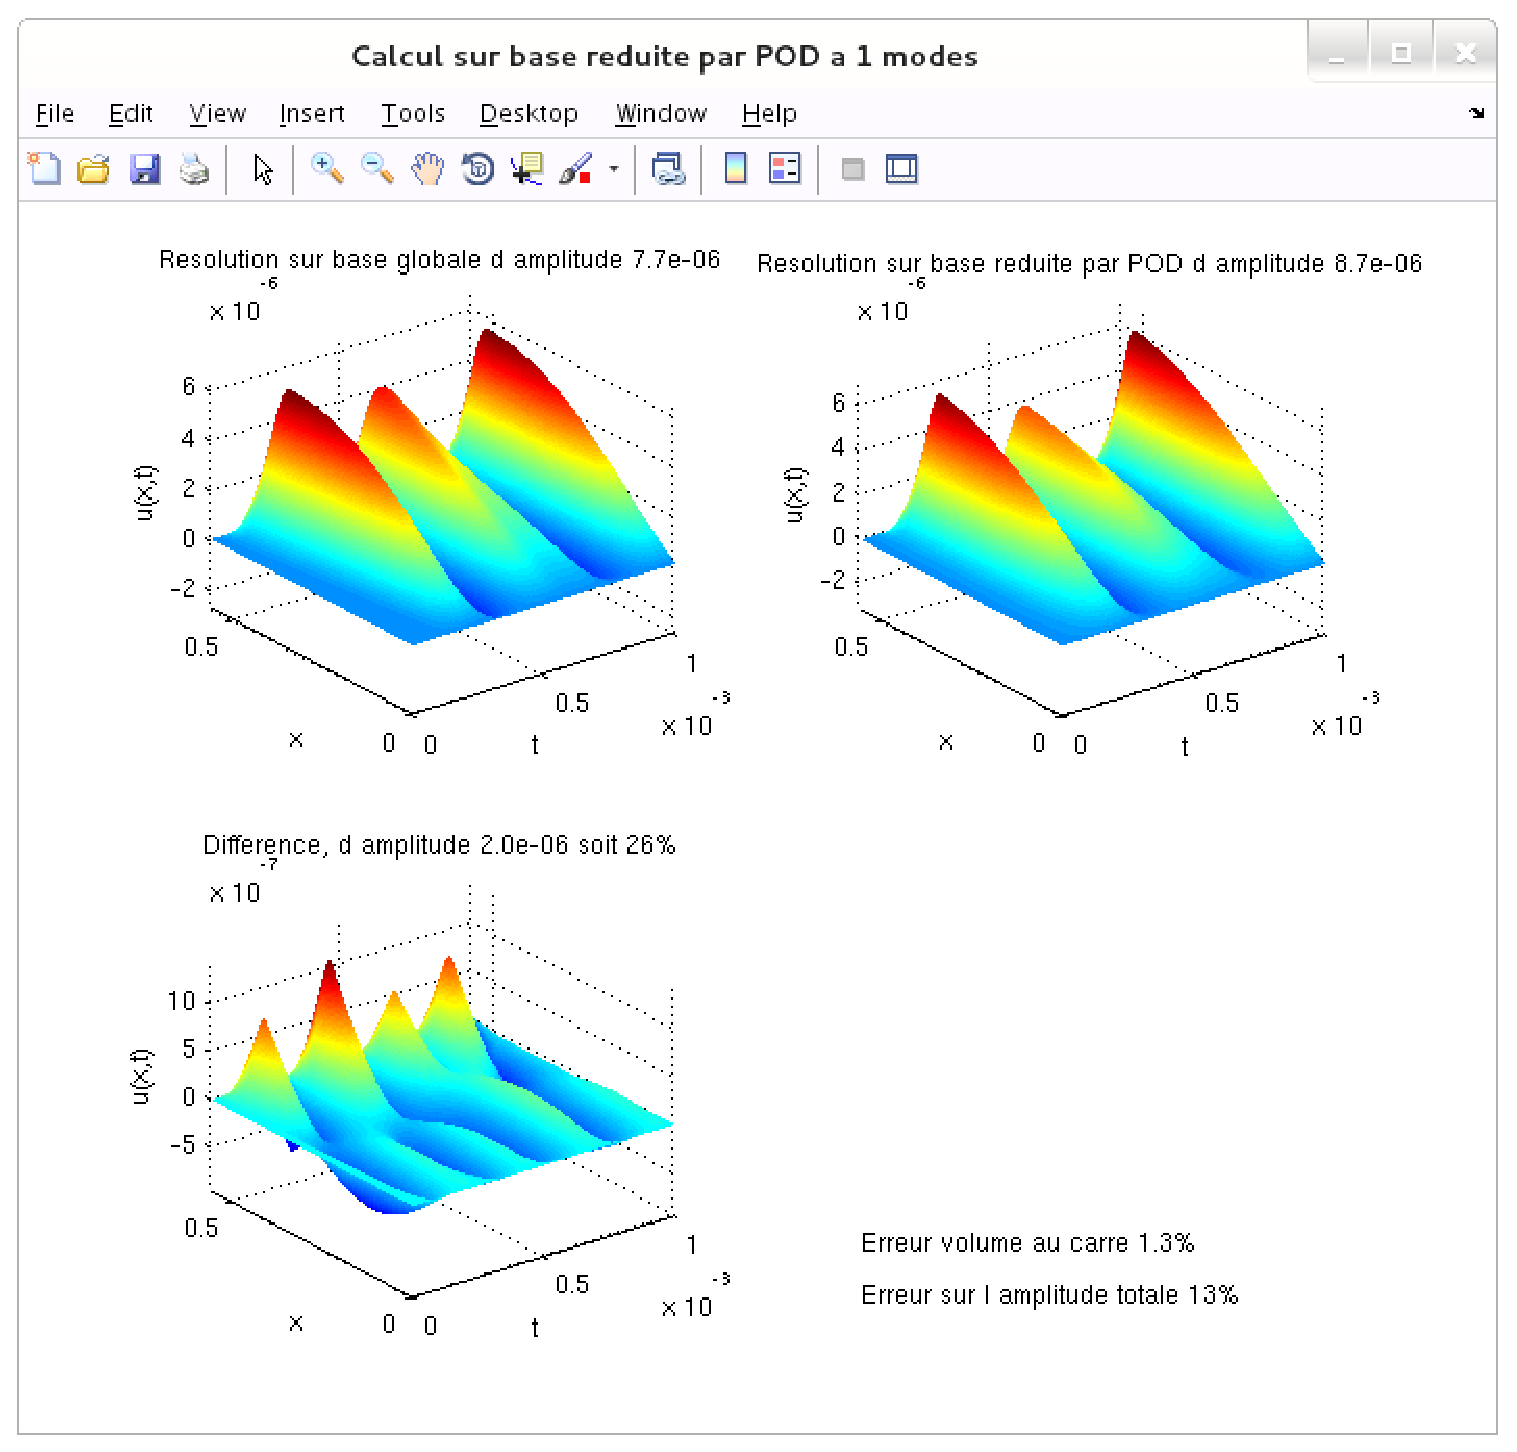
\includegraphics[width=0.68\linewidth]{Images/FenetreType.eps}
\caption{Fenêtre type de $Matblab$ \label{FenetreMatblabType}}
\end{figure}

\section{Méthode de Rayleigh-Ritz}
Cette méthode permettant d'avoir des modes espace, l'analyse par nombre de MAC a été mise en place pour pouvoir les comparer aux précédents. La méthode itérative utilisée est détaillée dans la partie \ref{IntroRR}, et il a pu être constaté que la forme de la matrice de masse choisie pouvait influé sur la convergence de cette méthode.

\section{PGD}
La difficulté particulière dans la programmation de la PGD est que le code n'est testable que globalement. 

Le code en place réalise une PGD à deux variables uniquement : espace et temps. Les modes en espace sont normalisés pour les raisons évoquées en \ref{ResultatsPGD}. Le besoin qui s'impose pour la résolution du problème en espace comme il est défini en \ref{ProbEspace}, est d'intégrer des produits de deux fonctions comme on peut le voir dans le déroulement des calculs en annexes \ref{IntegrDeProd}.

Quand la PGD est réalisée avec uniquement deux variables, il est possible de mettre en place un orthogonalisation (cela peut rester possible avec plus de variables mais devient plus complexe à mettre en place). Ceci permet d'avoir des modes indépendants et d'améliorer les modes calculer précédemment comme le montre l'annexe \ref{AlgorithmesPGDOrthoCorrect}. Comme au delà de deux variables, l'orthogonalisation pose des problèmes, et même si le code actuel n'en possède que deux, dans la perspective d'ajouter d'autres variables on ne va pas s'intéresser plus à l'orthogonalisation.

%\section{Ouverture}


\chapter{Résultats}

\section{Condensation}
Comme décrite dans la partie \ref{SectionCondensation}, la condensation repose sur le fait que l'inertie d'une partie des nœuds est négligeable. Elle semble donc inadaptée à un calcul sur un système ou la masse est répartie de manière homogène, comme ici. Et quand bien même il serait possible de répartir la masse des nœuds esclaves sur les nœuds maîtres (cela parait envisageable sur le problème poutre en utilisant une méthode non systématique), dans le meilleur des cas on retrouverait le système à résoudre comme si on avait discrétisé l'espace moins finement.


\section{Méthode Rayleigh-Ritz}
La méthode de Rayleigh-Ritz peut être plus rapide que la POD pour calculer des modes espace (La POD fournis en plus des modes en temps), selon la taille du snapshot* choisi pour la POD (*explication la partie suivante sur la POD). En comparant les modes POD et Rayleigh-Ritz par une analyse de MAC, on peut voir qu'il s'agit des mêmes si le snapshot choisi est suffisamment long. 

En revanche on atteint les limites de la méthode si l'on choisi d'introduire une non-linéarité ou un déplacement imposé qui varie au cours du temps. Ces faiblesses sont dues au fait que la méthode de Rayleigh-Ritz ne se base que sur les données initiales du système, la non-linéarité n'est donc pas visible ou bien il faut recalculer les modes comme expliquer dans la partie \ref{NonLinRR}. Le fait d'imposer un déplacement qui varie au cours du temps ne se voit pas dans la méthode Rayleigh-Ritz, et le ou les nœuds en question sont considérés comme encastrés, alors les modes trouvés ne décrivent pas la réponse du système de manière satisfaisante.

 
\section{POD}
Comme cela est expliqué dans la partie \ref{IntroPOD}, la POD repose sur une résolution préalable d'un problème sur base complète. On peut utiliser la réduction de modèle qu'elle apporte pour effectuer un grand nombre de calculs semblables ou pour calculer la réponse du système sur temps plus long. On appelle l'échantillon du temps sur lequel est faite la résolution préalable : le snapshot. Il représente un temps de calcul et donc un coût ce qui évidemment pousse à le choisir court. Mais la durée du snapshot conditionne aussi la qualité des modes trouvés par la SVD, et cela limite la volonté de le raccourcir. Dans le programme, la longueur du snapshot est choisi en fonction de la période du premier mode pour pouvoir observer quelques oscillations.

\section{PGD}
\label{ResultatsPGD}
La PGD fournis des modes en espace et en temps sans résolution préalable, fournis une solution, permet d'ajouter des paramètres, mais elle a quelques faiblesses. Notamment vis-à-vis de la convergence.

Premièrement à l'intérieur du point fixe : On peut observer que le point fixe ne converge pas toujours rapidement, et si on arrête le calcul du point fixe après un nombre fixe d'itérations ($k_{max}$ dans l'algorithme \ref{AlgoPGD} de la partie \ref{AlgoPGDPartie}) on peut trouver un mode défectueux qui va détériorer la solution globale voire empêcher sa convergence. Heureusement il est possible de remédier à ce problème en normalisant les fonctions en espace. On garde donc la forme du mode en espace mais pas son intensité, qui est répercuter sur la fonction en temps. Avec la normalisation il ne se manifeste plus de divergence cependant, la convergence du point fixe n'est pourtant pas assurée. 

Dans la figure \ref{ConvergenceDuPointFixe}, qui se base sur une résolution PGD d'un problème où l'on cherche la solution sous la forme d'une somme de produit de fonctions du temps et de fonctions de l'espace. La courbe est une indication de la convergence obtenue par la formule suivante calculer à chaque itération :

\begin{equation}
\left[
\frac{\displaystyle 
	\int_T \big(g_k(t) - g_{k-1}(t)\big)^2 dt  
		~~\big((\boldsymbol{\varphi_q})_k - (\boldsymbol{\varphi_q})_{k-1}\big)^T 
						\mathbf{K} 
		  \big((\boldsymbol{\varphi_q})_k - (\boldsymbol{\varphi_q})_{k-1}\big)
}
{\displaystyle 
\int_T g_k(t)^2 dt
	~~(\boldsymbol{\varphi_q})_k^T \mathbf{K} (\boldsymbol{\varphi_q})_k
} 
\right]^\frac{1}{2}
\end{equation}

ce qui correspond à :

\begin{equation}
\frac{\displaystyle 
	\big\Vert (g_k(t) - g_{k-1})\big\Vert_T 
		~~\big\Vert (\boldsymbol{\varphi_q})_k 
					- (\boldsymbol{\varphi_q})_{k-1} \big\Vert_\Omega
}
{\displaystyle 
	\big\Vert g_k(t) \big\Vert_T 
		~~\big\Vert (\boldsymbol{\varphi_q})_k \big\Vert_\Omega 
} 
\end{equation}


\begin{figure}[!ht]
\centering
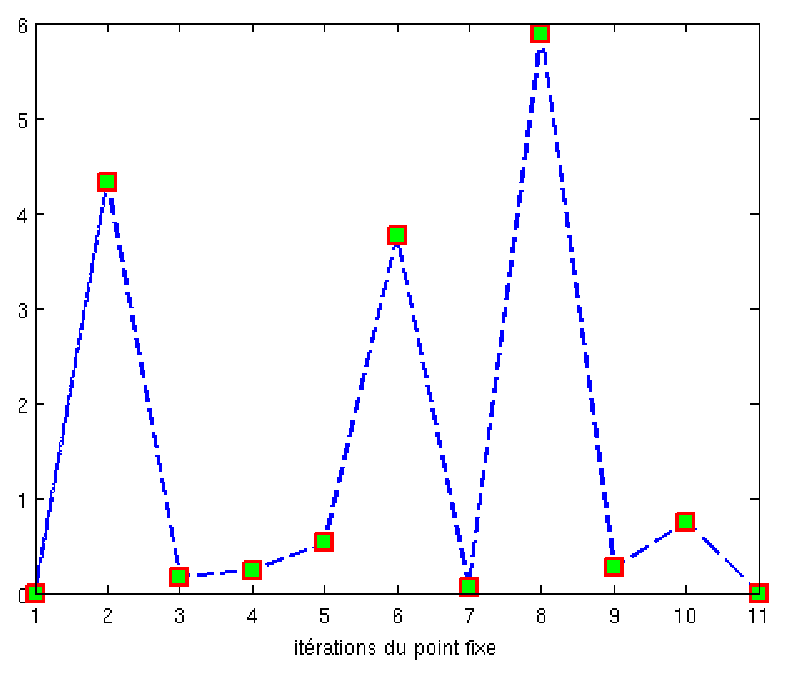
\includegraphics[width=0.425\linewidth]{Images/ConvergenceDuPointFixeAvecNormMode14.eps}
\caption{Convergence du point fixe au $14^e$ mode \label{ConvergenceDuPointFixe}}
\end{figure}

Sur la figure \ref{ConvergenceDuPointFixe} on voit que même après $8$ itérations du point fixe le mode peut subir de grande variations. Le mode a été choisi pour illustrer le problème mais la plus part des modes stagnent (convergent) après quelques itérations. Dans le cas où un point fixe ne converge pas, on compte sur les modes suivants pour corriger l'apport défectueux. Ceci semble fonctionner à condition de normer les fonctions d'espace.

Sur la figure \ref{DiminutionDeLErreurPGD} sont affichés deux indicateurs d'erreur de la solution PGD par rapport à la solution de référence éléments finis. La courbe en bleu représente l'erreur sur l'amplitude totale du signal. La courbe rouge en pointillés représente le maximum de l'erreur. Les formules sont données dans la partie \ref{EquationErreurPartie}, respectivement l'équation \ref{EquationErreurAmp} et l'équation \ref{EquationErreurMax}.

\begin{figure}[!ht]
\centering
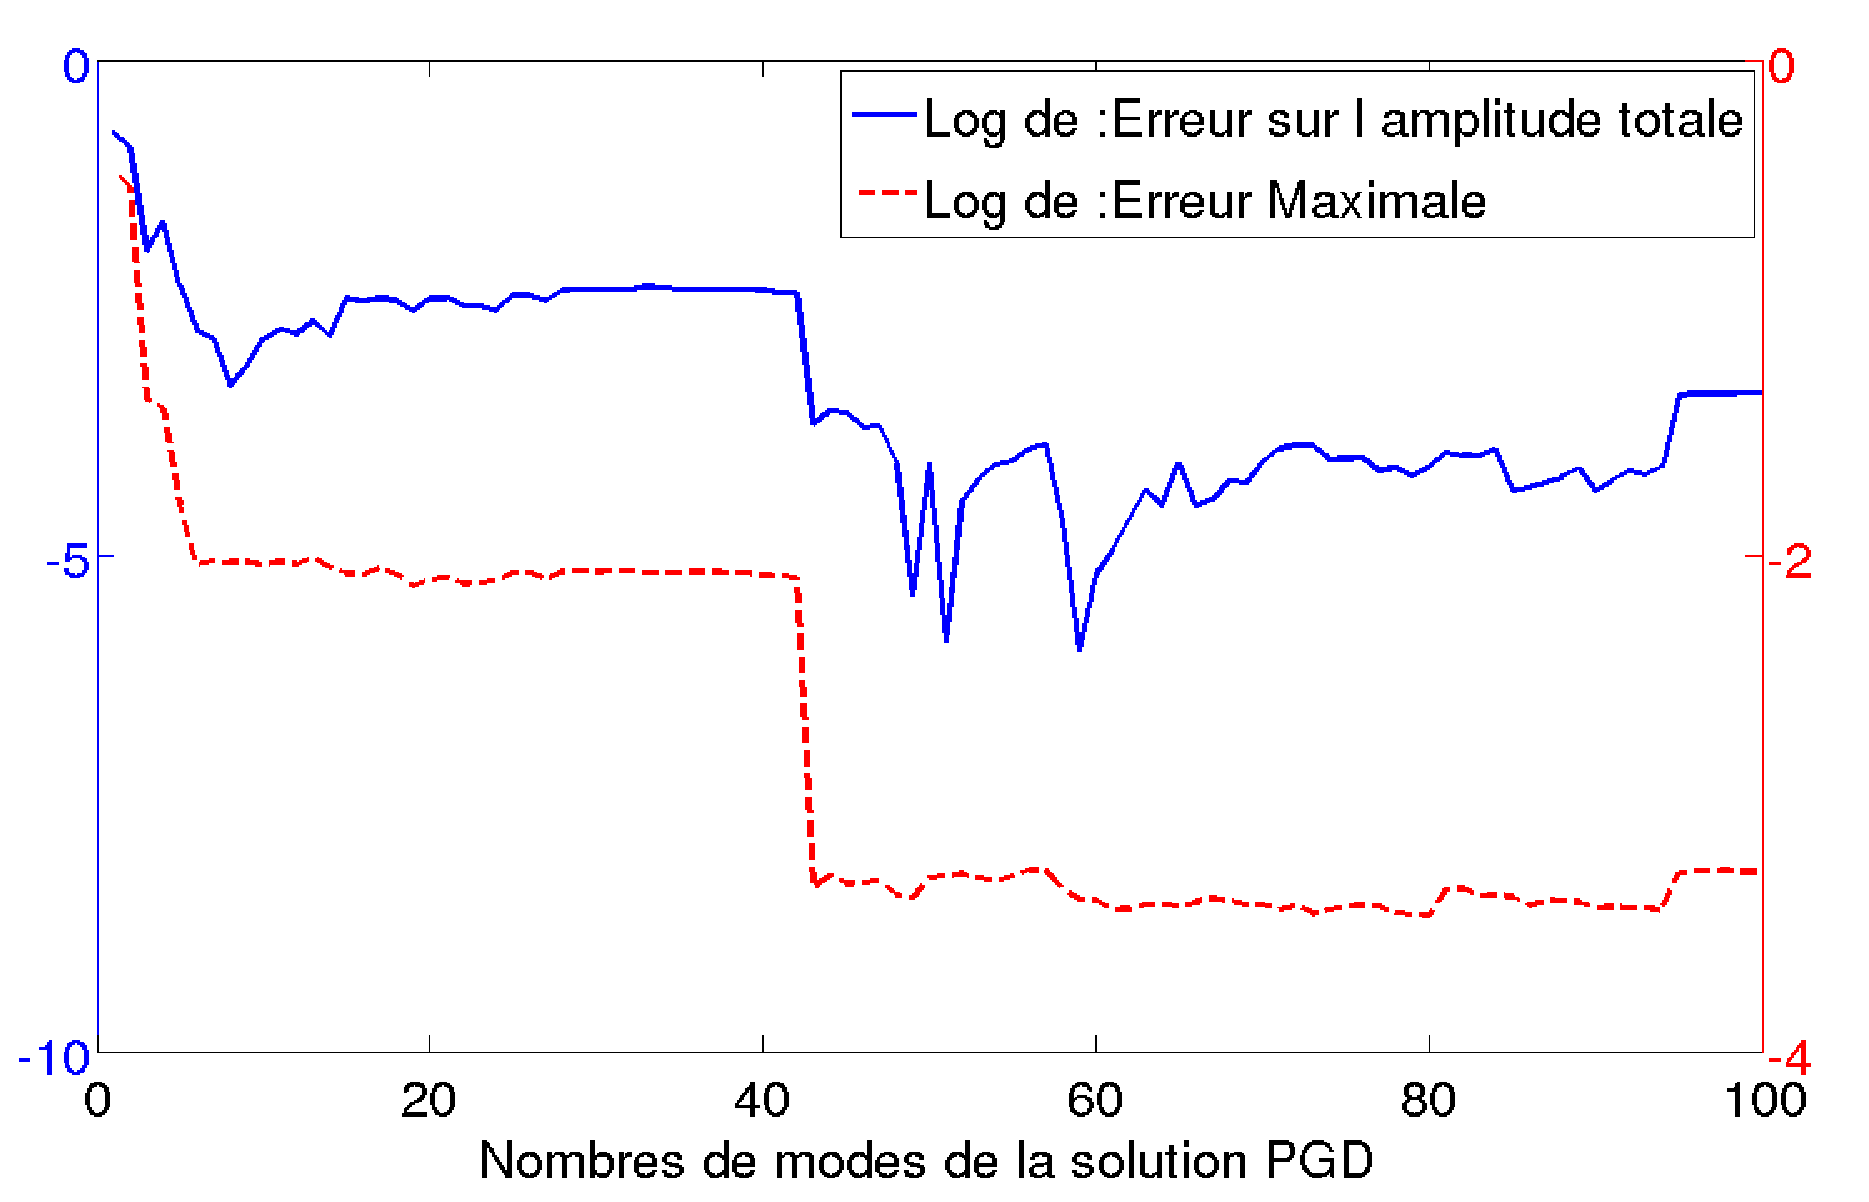
\includegraphics[width=0.7\linewidth]{Images/100ModesPGDAvecNormNonAmorti.eps}
\caption{Évolution des indicateurs d'erreur d'une solution PGD \label{DiminutionDeLErreurPGD}}
\end{figure}

La courbe bleu étant sujet à de nombreuses fluctuations, on peut observer plus nettement la diminution de l'erreur sur la courbe rouge. On peut aussi remarquer que tous les modes n'ont pas une contribution de même importance à la diminution de l'erreur. En effet en l'absence d'orthogonalisation des modes, les nouveaux modes trouvés par l'algorithme peuvent être plus moins colinéaires aux modes déjà présent dans la base PGD.

La figure \ref{DiminutionDeLErreurPOD} représente les mêmes quantités que la précédente mais évaluées pour des solutions calculées par réduction de modèle par POD en faisant varier le nombre de modes. Évidemment la POD fournis des résultats d'erreur moindre pour un même nombre de modes, mais il y a une différence majeure entre la réalisation de ces deux figures : Dans le cas de la PGD, pour avoir un mode supplémentaire on fait juste converger le point fixe une fois de plus. Alors que pour la POD l'ajout d'un mode agrandis la base de projection et pour avoir la nouvelle solution il faut résoudre entièrement le problème sur cette nouvelle base.

\begin{figure}[!ht]
\centering
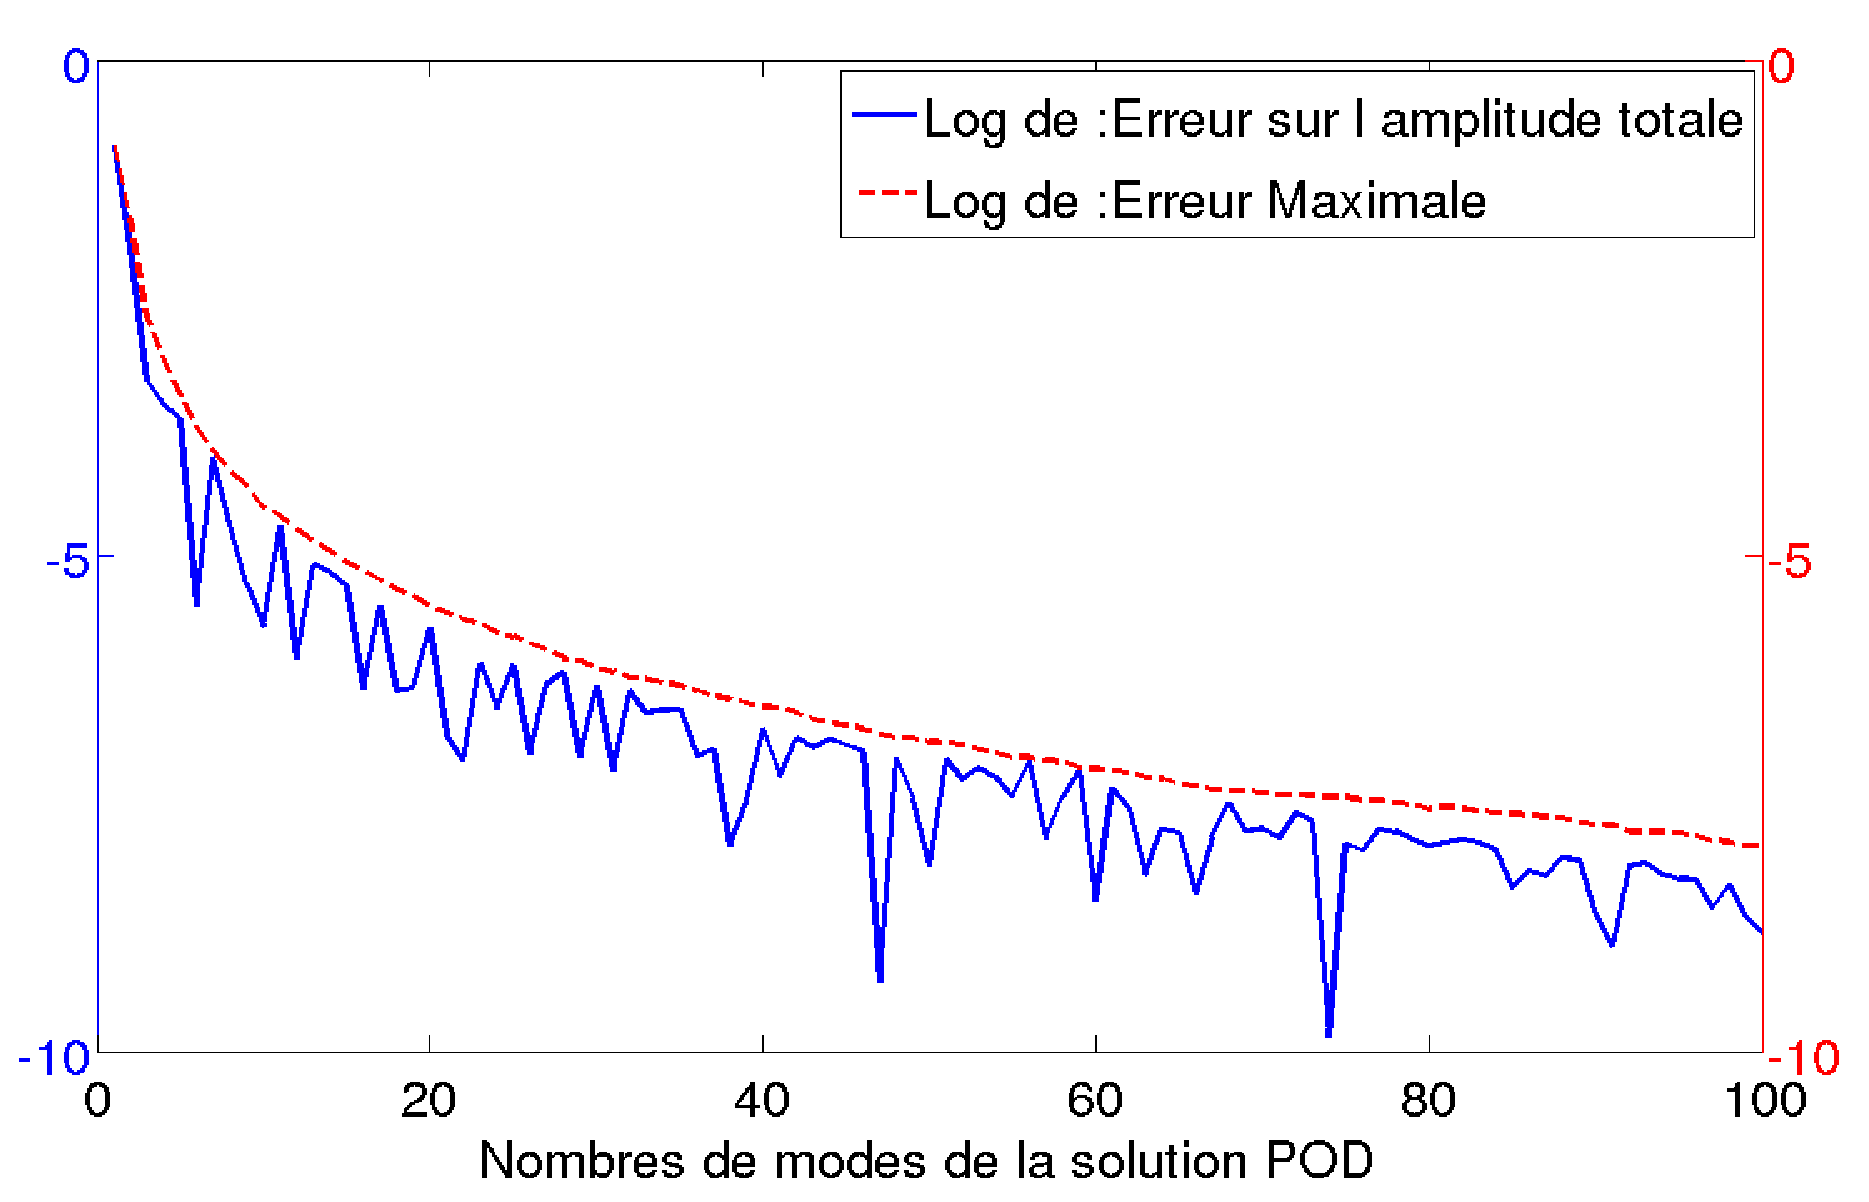
\includegraphics[width=0.7\linewidth]{Images/100ModesPOD.eps}
\caption{Évolution des indicateurs d'erreur d'une solution POD \label{DiminutionDeLErreurPOD}}
\end{figure}

Sur la figure \ref{AnalyseDeMAC} est représentée la comparaison des modes PGD aux modes POD par analyse de MAC. On peut voir qu'après une centaine de modes trouvés par la PGD, on représente en réalité moins d'une quinzaine de modes indépendants (orthogonaux), qui correspondent au premiers modes de la POD. Pour remédier à ce problème il faudrait orthogonaliser les modes. Mais comme expliqué précédemment, l'orthogonalisation ne sera pas mise en place.

\begin{figure}[!ht]
\centering
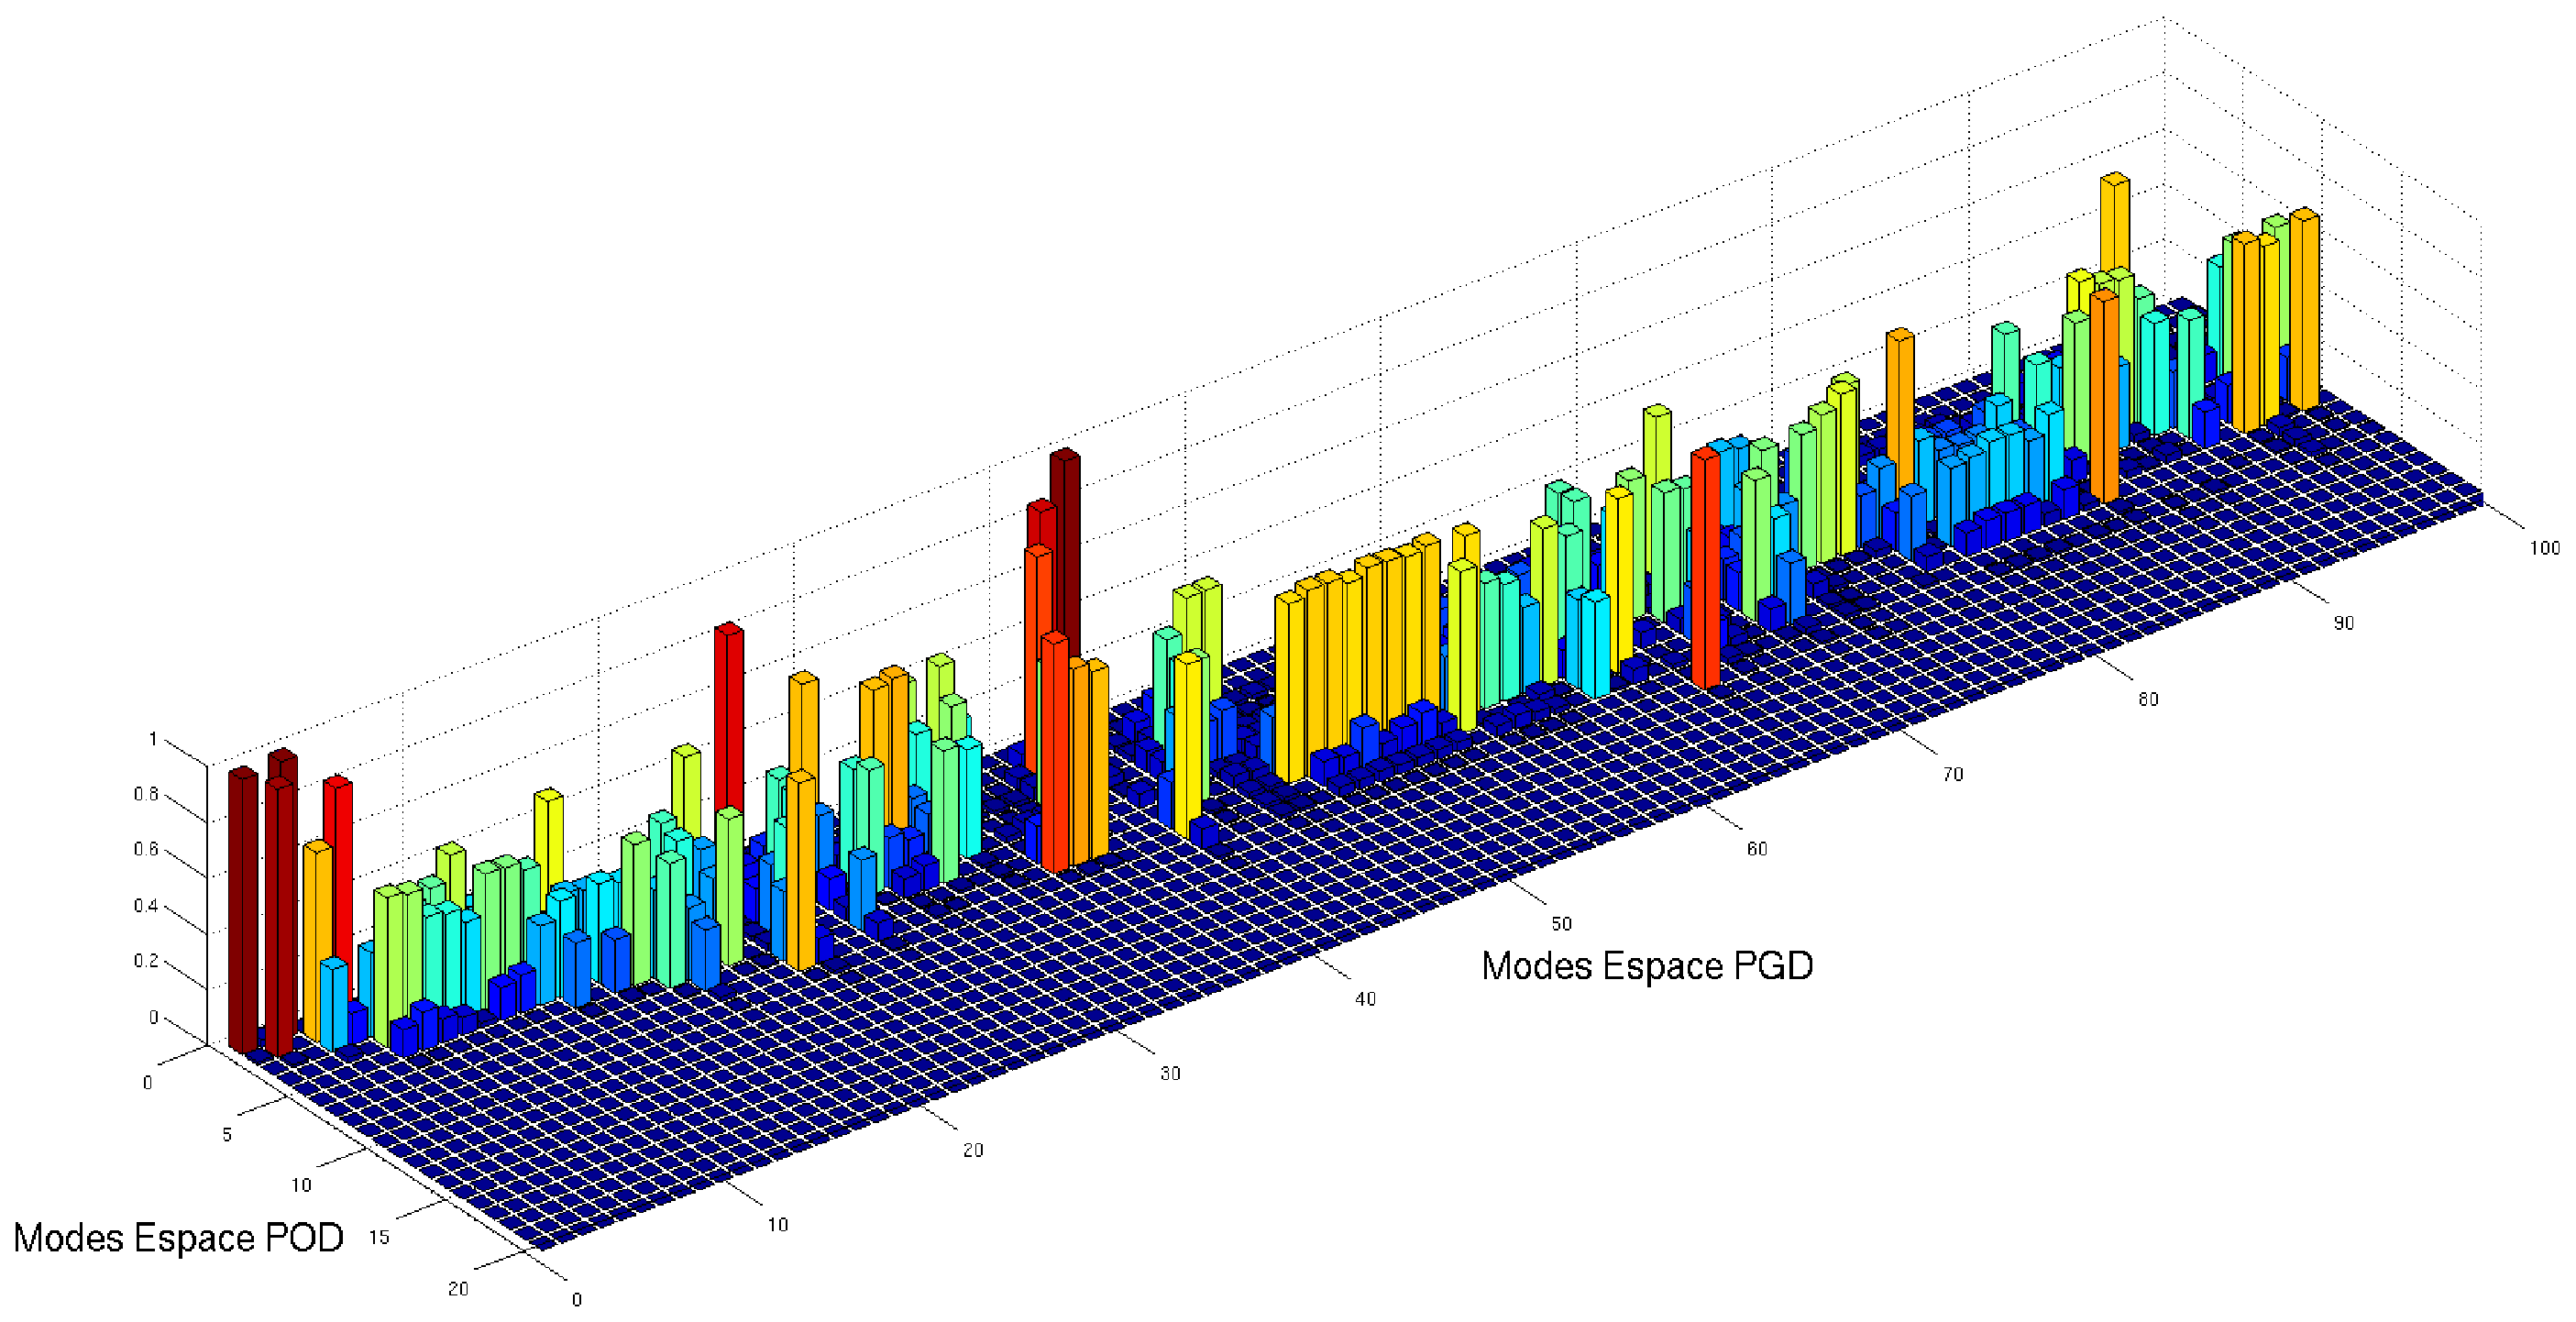
\includegraphics[width=0.8\linewidth]{Images/100ModesAvecNormNonAmortiMAC.eps}
\caption{Comparaisons des modes PGD et POD \label{AnalyseDeMAC}}
\end{figure}





\chapter{La PDG pour les problèmes de dynamique non-linéaire}
Les problèmes non-linéaires posent des problèmes de résolution car l'absence de linéarité proscrit l'utilisation de nombreux théorèmes comme celui de Lax-Milgram décrit en partie \ref{LaxMilgram}, puisqu'elle contredit ses hypothèses. Les algorithmes de résolution appliqués aux problèmes linéaires perdent donc ici des propriétés de convergence et c'est pour étendre les possibilités de résolution des problèmes non-linéaires qu'a été développée la méthode
LATIN.

\section{La Méthode LATIN}
Introduite par \cite{LATIN1} et \cite{LATIN2}, la méthode LATIN (pour LArge Time INcrement) a permis d'établir la
convergence de résolutions pour des problèmes mettant en jeu des matériaux non-linéaires
à la condition qu'ils respectent l'inégalité de Drucker:
\begin{equation}
\oint_C \sigma d\varepsilon \geq 0, \forall C
\end{equation}

Cette inégalité se traduit par la positivité du travail plastique, puisque le travail des contraintes est nul sur un trajet élastique (pour un trajet fermé). Ceci comprend de nombreux matériaux plastiques ou viscoplastiques. Cette méthode atteint ses limites en revanche pour des matériaux instables, et notamment les matériaux dommageables, pour lesquels la convergence n'est pas assurée. Son nom lui vient du fait qu'elle permet de résoudre des problèmes en temps sur l'ensemble du domaine temporel. Cette capacité a été apportée par la formulation qui est à l'origine de la PGD, utilisant la séparation des variables. La méthode LATIN est itérative puisqu'elle se base sur la résolution alternative de deux problèmes dont l'un et local est potentiellement non-linéaire, et l'autre est linéaire et potentiellement global. Pour plus de détails voir \cite{LATIN2} et \cite{LATINmultiscale}. La PGD est utilisée pour résoudre le problème linéaire, ce qui est particulièrement pertinent quand la solution de ce problème ne change que légèrement d'une itération à l'autre. L'objectif du travail qui suivra cette bibliographie est d'étudier la possibilité de l'utiliser même pour des problèmes non-linéaires.

\section{Les Résolutions non-linéaires}
\subsection{Condensation}
Une méthode de condensation traitant des problèmes non-linéaire est décrite par \cite{ERMT}, mais se limite à une utilisation dans le cas d'éléments linéaires connectés de manière non- linéaire. La méthode développée dans cette article (SEREP) permet de conserver les valeurs propres et vecteurs propres dans le modèle réduit.
\subsection{Rayleigh-Ritz}
\label{NonLinRR}
Le code Aster propose un extension de la méthode de Rayleigh-Ritz à des cas non-linéaires. Le problème est alors formulé ainsi :
\[
\mathbf{M}\mathbf{\ddot{u}} + \mathbf{K}(\mathbf{u}) = \mathbf{f}
\]

$\mathbf{K}(\mathbf{u})$ est une fonction non linéaire qui dépend des déplacements, tel une raideur non linéaire ou un contact. Alors on définit une matrice de rigidité tangente :
\[
\mathbf{\mathbf{K}^{tg}} u =
\partial H(u)
\partial u
\]
On définit alors une base modale à l'aide de modes solution de l'équation :
\[
\left( \mathbf{\mathbf{K}^{tg}} \mathbf{u} 
	- \omega^{tg}_i \mathbf{M} 
\right) \boldsymbol{\varphi^{tg}_i} = 0
\]
Ces modes dépendent de $\mathbf{\mathbf{K}^{tg}}$ et donc de $\mathbf{u}$.
\subsection{POD}
La SVD peut permettre de décomposer un opérateur, mais si le problème se présente comme dans ce qui précède, il devra subir la décomposition pour chaque u donc à chaque pas de temps.
\section{Ouverture}
La PDG non linéaire est un domaine de recherche qui est tout à fait d'actualité, puisque l'application de la PGD à des problèmes non-linéaires fait l'objet de travaux en cours ou à publier comme \cite{performante} et \cite{fonderie}, qui présente des problèmes liés à la thermique non-linéaire. Ceci sera l'objet de l'étude du travail qui suivra.


\addcontentsline{toc}{part}{Bibliographie} 
\bibliographystyle{unsrt}
\bibliography{References}

\newpage

\appendix
\chapter{Remerciements}

\paragraph{Mes encadrants} 
Je voudrais remercier Francois \bsc{Louf} et Pierre-Alain \bsc{Boucard}, pour m'avoir orienté, aidé et avoir répondu à mes nombreuses questions autant par e-mail que de vive voix.

\paragraph{Mes collègues}
Je remercie mes collègues de master pour l'aide donné comme reçue, que se soit pour des réflexions théoriques ou dans la recherche d'une syntaxe $Matlab$ ou \LaTeX. Et je les remercie aussi pour avoir maintenue une ambiance agréable dans une salle souterraine.

\paragraph{Le LMT}
Ce stage c'est bien passé aussi grâce au laboratoire, qui non-seulement a mis à ma disposition un poste mais me permet de détendre au bar et lors d'éventuel évènements. J'espère que les choses continueront ainsi en thèse.

\paragraph{Wilson} La mascotte de la salle master 2.


\chapter{Compression d'image par SVD}
  \lstset {
  caption={Traitement d'image par SVD}}
\lstinputlisting[language=Matlab]{Images/SVD/test2.m}

\chapter{Calcul du problème PGD étape par étape}
%\documentclass[10pt]{report}
%
%\begin{document}
\begin{itemize}
\item Admissibilité cinématique :
	\\$U \in [H^1(\Omega)]^3, U_{|\partial \Omega_U} = U_d $
\item Admissibilité statique :
	\\$ div \sigma + f_v = \rho \ddot{U} + \mu \dot{U}$ sur $\Omega$ 
		et $\sigma . n _{|\partial \Omega_f} = f_d$
\item Relation de comportement :
	\\$\sigma = H : \epsilon (U)$ sur $ \Omega$
\item Conditions initiales :
	\\$U(0) = U_0$ et $ \dot{U}(0) = \dot{U}_0$
\end{itemize}

\noindent
Formulation variationnelle : 
\begin{equation}
	\forall U^* ~ \text{CA0,} ~
		\int_\Omega [\epsilon (U^*) : \sigma   
					+ U^* \mu \dot{U} 
					+ U^* \rho \ddot{U}
					- U^* f_d
					] d \Omega	
		- \int_{\partial \Omega_f} U^* f_d  ds		
		- \underbrace{
			\int_{\partial \Omega_U} U^* \sigma . n ds	
		  }_{=0}
		= 0
\end{equation}

\noindent
Où
\begin{itemize}
\item $U$ est le déplacement
\item $\Omega$ l'espace, avec le bord $\partial \Omega = \partial \Omega_U \cap \partial \Omega_f$
\item $\sigma$ le tenseur des contraintes
\item $\epsilon$ le tenseur des déformations
\item $\rho$ la masse volumique
\item $\mu$ expression de la viscosité (cette donnée est généralement mal connue)
\item $H$ le tenseur de Hook
\item $f_v$ effort volumique
\item $f_d$ effort imposé que le bord de $\Omega$
\end{itemize}
\vspace{0.3cm}

\noindent
Mise en place de la PGD, utilisation de l'hypothèse des variables séparables :
\begin{equation}
	U(x,t,\theta) = \sum_{k=1}^n \phi_k(x) g_k(t)h_k(\theta)
\end{equation}

Pour chaque $k$, il faut discrétiser les fonctions sur leur domaine de définition : 
\begin{equation}
	\begin{array}{l c l c l}
		\phi(x) &=& \sum_{i=1}^{Nbc_x}  N_i (x) \phi_i &=& N_\phi(x) \boldsymbol{\phi_q}
		\\
		g(t) &=& \sum_{i=1}^{Nbc_t}  N_i (t) gi &=& N_g(t) \mathbf{g_q}
		\\
		h(\theta) &=& \sum_{i=1}^{Nbc_\theta}  N_i (\theta) hi 
		&=& N_h(\theta) \mathbf{h_q}
	\end{array}
\end{equation}
$Nbc_x$ Représente le nombre de composante de discrétisation spatiale, l'indice $q$ représente le vecteur sur le domaine discrétisé.
\\
On remplace dans la formulation variationnelle, en choisissant $U^* = (\phi gh)^* = ( \phi^*gh+\phi g^*h+\phi gh^*) $ :
\begin{equation}
\begin{array}{r r l}
	&\int_\Omega \! \int_T \! \int_\Theta \!\!\!&		
		[\epsilon (\phi^*gh) : H : \epsilon (U_n)
			+ \phi^*gh \mu \dot{U_n} 
			+ \phi^*gh \rho \ddot{U_n}
			- \phi^*gh f_v
			] ~dx dt d\theta
	\\
	+ &\int_\Omega \! \int_T \! \int_\Theta \!\!\!&		
		[\epsilon (\phi g^*h) : H : \epsilon (U_n)
			+ \phi g^*h \mu \dot{U_n} 
			+ \phi g^*h \rho \ddot{U_n}
			- \phi g^*h f_v
			] ~dx dt d\theta
	\\
	+ &\int_\Omega \! \int_T \! \int_\Theta \!\!\!&		
		[\epsilon (\phi gh^*) : H : \epsilon (U_n)
			+ \phi gh^* \mu \dot{U_n} 
			+ \phi gh^* \rho \ddot{U_n}
			- \phi gh^* f_v
			] ~dx dt d\theta
	\\
	- &\int_{\partial \Omega_\mathbf{f}} \! \int_T \! \int_\Theta \!\!\!&
		(\phi^*gh + \phi g^*h + \phi gh^*) f_d  ~ds dt d\theta
\\
	= &0& 
\end{array}
\end{equation}

Puis $U = U_{n} = U_{n-1} + \phi gh$ :
\begin{equation}
\begin{array}{r r l}
	&\int_\Omega \! \int_T \! \int_\Theta \!\!\!&		
		gh[\epsilon (\phi^*) : H : \epsilon (U_{n-1} + \phi gh)
			+ \phi^* \mu \dot{(U_{n-1} + \phi gh)} 
			+ \phi^* \rho \ddot{(U_{n-1} + \phi gh)}
			- \phi^* f_v
			] ~dx dt d\theta
	\\
	+ &\int_\Omega \! \int_T \! \int_\Theta \!\!\!&		
		g^*h[\epsilon (\phi) : H : \epsilon (U_{n-1} + \phi gh)
			+ \phi \mu \dot{(U_{n-1} + \phi gh)} 
			+ \phi \rho \ddot{(U_{n-1} + \phi gh)}
			- \phi f_v
			] ~dx dt d\theta
	\\
	+ &\int_\Omega \! \int_T \! \int_\Theta \!\!\!&		
		gh^*[\epsilon (\phi) : H : \epsilon (U_{n-1} + \phi gh)
			+ \phi \mu \dot{(U_{n-1} + \phi gh)} 
			+ \phi \rho \ddot{(U_{n-1} + \phi gh)}
			- \phi f_v
			] ~dx dt d\theta
	\\
	- &\int_{\partial \Omega_\mathbf{f}} \! \int_T \! \int_\Theta \!\!\!&
		(\phi^*gh + \phi g^*h + \phi gh^*) f_d  ~ds dt d\theta
\\
	= &0& 
\end{array}
\end{equation}

On distribue la dérivation : 
\begin{equation}
\begin{array}{r r l}
	&\int_\Omega \! \int_T \! \int_\Theta \!\!\!&		
		gh[\epsilon (\phi^*) : H : \epsilon (U_{n-1} + \phi gh)
			+ \phi^* \mu (\dot{U_{n-1}} + \phi \dot{g}h)
			+ \phi^* \rho (\ddot{U_{n-1}} + \phi \ddot{g}h)
			- \phi^* f_v
			] ~dx dt d\theta
	\\
	+ &\int_\Omega \! \int_T \! \int_\Theta \!\!\!&		
		g^*h[\epsilon (\phi) : H : \epsilon (U_{n-1} + \phi gh)
			+ \phi \mu (\dot{U_{n-1}} + \phi \dot{g}h) 
			+ \phi \rho (\ddot{U_{n-1}} + \phi \ddot{g}h)
			- \phi f_v
			] ~dx dt d\theta
	\\
	+ &\int_\Omega \! \int_T \! \int_\Theta \!\!\!&		
		gh^*[\epsilon (\phi) : H : \epsilon (U_{n-1} + \phi gh)
			+ \phi \mu (\dot{U_{n-1}} + \phi\dot{g}h)
			+ \phi \rho (\ddot{U_{n-1}} + \phi\ddot{g}h)
			- \phi f_v
			] ~dx dt d\theta
	\\
	- &\int_{\partial \Omega_\mathbf{f}} \! \int_T \! \int_\Theta \!\!\!&
		(\phi^*gh + \phi g^*h + \phi gh^*) f_d  ~ds dt d\theta
\\
	= &0& 
\end{array}
\end{equation}

On sépare les termes en $n-1$ des termes virtuels :
\begin{equation}
\begin{array}{r r l}
	&\int_\Omega \! \int_T \! \int_\Theta \!\!\!&		
		gh[\epsilon (\phi^*) : H : \epsilon (\phi gh)
			+ \phi^* \mu \phi\dot{g}h
			+ \phi^* \rho \phi\ddot{g}h
			- \phi^* f_v
			] ~dx dt d\theta
	\\
	+ &\int_\Omega \! \int_T \! \int_\Theta \!\!\!&		
		gh[\epsilon (\phi^*) : H : \epsilon (U_{n-1})
			+ \phi^* \mu \dot{U_{n-1}} 
			+ \phi^* \rho \ddot{U_{n-1}}
			] ~dx dt d\theta
	\\
	+ &\int_\Omega \! \int_T \! \int_\Theta \!\!\!&		
		g^*h[\epsilon (\phi) : H : \epsilon ( \phi gh)
			+ \phi \mu  \phi\dot{g}h
			+ \phi \rho \phi\ddot{g}h
			- \phi f_v
			] ~dx dt d\theta
	\\
	+ &\int_\Omega \! \int_T \! \int_\Theta \!\!\!&		
		g^*h[\epsilon (\phi) : H : \epsilon (U_{n-1})
			+ \phi \mu \dot{U_{n-1}}
			+ \phi \rho \ddot{U_{n-1}}
			] ~dx dt d\theta
	\\
	+ &\int_\Omega \! \int_T \! \int_\Theta \!\!\!&		
		gh^*[\epsilon (\phi) : H : \epsilon (\phi gh)
			+ \phi \mu + \phi\dot{g}h
			+ \phi \rho \phi\ddot{g}h
			- \phi f_v
			] ~dx dt d\theta
	\\
	+ &\int_\Omega \! \int_T \! \int_\Theta \!\!\!&		
		gh^*[\epsilon (\phi) : H : \epsilon (U_{n-1})
			+ \phi \mu \dot{U_{n-1}}
			+ \phi \rho \ddot{U_{n-1}}
			- \phi f_v
			] ~dx dt d\theta
	\\
	- &\int_{\partial \Omega_\mathbf{f}} \! \int_T \! \int_\Theta \!\!\!&
		(\phi^*gh + \phi g^*h + \phi gh^*) f_d  ~ds dt d\theta
	\\
	= &0& 
\end{array}
\end{equation}

On peut regrouper les termes qui n'ont pas de partie virtuel en espace i.e. $\phi^*$ :
\begin{equation}
\begin{array}{r r l}
	&\int_\Omega \! \int_T \! \int_\Theta \!\!\!&		
		gh[\epsilon (\phi^*) : H : \epsilon (\phi gh)
			+ \phi^* \mu \phi\dot{g}h
			+ \phi^* \rho \phi\ddot{g}h
			- \phi^* f_v
			] ~dx dt d\theta
	\\
	+ &\int_\Omega \! \int_T \! \int_\Theta \!\!\!&		
		gh[\epsilon (\phi^*) : H : \epsilon (U_{n-1})
			+ \phi^* \mu \dot{U_{n-1}} 
			+ \phi^* \rho \ddot{U_{n-1}}
			] ~dx dt d\theta
	\\
	+ &\int_\Omega \! \int_T \! \int_\Theta \!\!\!&		
		(g^*h + gh^*)[\epsilon (\phi) : H : \epsilon ( \phi gh)
			+ \phi \mu  \phi\dot{g}h
			+ \phi \rho \phi\ddot{g}h
			- \phi f_v
			] ~dx dt d\theta
	\\
	+ &\int_\Omega \! \int_T \! \int_\Theta \!\!\!&		
		(g^*h + gh^*)[\epsilon (\phi) : H : \epsilon (U_{n-1})
			+ \phi \mu \dot{U_{n-1}}
			+ \phi \rho \ddot{U_{n-1}}
			] ~dx dt d\theta
	\\
	- &\int_{\partial \Omega_\mathbf{f}} \! \int_T \! \int_\Theta \!\!\!&
		(\phi^*gh + \phi g^*h + \phi gh^*) f_d  ~ds dt d\theta
	\\
	= &0& 
\end{array}
\end{equation}

On discrétise en espace :
\begin{equation}
\begin{array}{r r l}
	&\int_\Omega \! \int_T \! \int_\Theta \!\!\!&		
		gh\boldsymbol{\phi_q}^*[\epsilon (N_\phi(x)) : H : \epsilon (N_\phi(x)\boldsymbol{\phi_q} gh)
			+ N_\phi(x) \mu  N_\phi(x) \boldsymbol{\phi_q}  \dot{g}h
			\\ && \phantom{gh\boldsymbol{\phi_q}^*[ }
			+ N_\phi(x) \rho N_\phi(x) \boldsymbol{\phi_q} \ddot{g}h
			- N_\phi(x) f_v
			] ~dx dt d\theta
	\\
	+ &\int_\Omega \! \int_T \! \int_\Theta \!\!\!&		
		gh\boldsymbol{\phi_q}^*[\epsilon (N_\phi(x)) : H : \epsilon (U_{n-1})
			+ N_\phi(x) \mu \dot{U_{n-1}} 
			+ N_\phi(x) \rho \ddot{U_{n-1}}
			] ~dx dt d\theta
	\\
	+ &\int_\Omega \! \int_T \! \int_\Theta \!\!\!&		
		(g^*h + gh^*)\boldsymbol{\phi_q}[\epsilon (N_\phi(x)) : H : \epsilon (N_\phi(x) \boldsymbol{\phi_q}gh)
			+ N_\phi(x) \mu  N_\phi(x) \boldsymbol{\phi_q} \dot{g}h
			\\ && \phantom{(g^*h + gh^*)\boldsymbol{\phi_q}[ }
			 + N_\phi(x) \rho N_\phi(x) \boldsymbol{\phi_q} \ddot{g}h
			- N_\phi(x) f_v
			] ~dx dt d\theta
	\\
	+ &\int_\Omega \! \int_T \! \int_\Theta \!\!\!&		
		(g^*h + gh^*)\boldsymbol{\phi_q}[\epsilon (N_\phi(x)) : H : \epsilon (U_{n-1})
			+ N_\phi(x) \mu \dot{U_{n-1}}
			+ N_\phi(x) \rho \ddot{U_{n-1}}
			] ~dx dt d\theta
	\\
	- &\int_{\partial \Omega_\mathbf{f}} \! \int_T \! \int_\Theta \!\!\!&
		N_\phi(x)(\boldsymbol{\phi_q}^*gh + \boldsymbol{\phi_q} g^*h + \boldsymbol{\phi_q} gh^*) f_d  ~ds dt d\theta
	\\
	= &0& 
\end{array}
\end{equation}

\begin{equation}
U_{n-1}(x,t,\theta)
	 = \sum_{k=1}^{n-1} \phi_k(x) g_k(t)h_k(\theta)
	 = \sum_{k=1}^{n-1} N_\phi(x)(\boldsymbol{\phi_q})_k g_k(t)h_k(\theta)
\end{equation}

En utilisant la formule précédente :
\begin{equation}
\begin{array}{r r l}
	&\int_\Omega \! \int_T \! \int_\Theta \!\!\!&		
		gh\boldsymbol{\phi_q}^*[\epsilon (N_\phi(x)) : H : \epsilon (N_\phi(x)\boldsymbol{\phi_q} gh)
			\\ && \phantom{gh\boldsymbol{\phi_q}^*[ }
			+ N_\phi(x) \mu  N_\phi(x) \boldsymbol{\phi_q}  \dot{g}h
			\\ && \phantom{gh\boldsymbol{\phi_q}^*[ }
			+ N_\phi(x) \rho N_\phi(x) \boldsymbol{\phi_q} \ddot{g}h
			- N_\phi(x) f_v
			] ~dx dt d\theta
	\\
	+ &\int_\Omega \! \int_T \! \int_\Theta \!\!\!&		
		gh\boldsymbol{\phi_q}^*[\epsilon (N_\phi(x)) : H : 
				\epsilon (\sum_{k=1}^{n-1} N_\phi(x)(\boldsymbol{\phi_q})_k g_k h_k)
			\\ && \phantom{gh\boldsymbol{\phi_q}^*[}
			+ N_\phi(x) \mu \sum_{k=1}^{n-1} N_\phi(x)(\boldsymbol{\phi_q})_k \dot{g_k} h_k 
			\\ && \phantom{gh\boldsymbol{\phi_q}^*[}
			+ N_\phi(x) \rho \sum_{k=1}^{n-1} N_\phi(x)(\boldsymbol{\phi_q})_k \ddot{g_k} h_k 
			] ~dx dt d\theta
	\\
	+ &\int_\Omega \! \int_T \! \int_\Theta \!\!\!&		
		(g^*h + gh^*)\boldsymbol{\phi_q}[\epsilon (N_\phi(x)) : H : \epsilon (N_\phi(x) \boldsymbol{\phi_q}gh)
			\\ && \phantom{(g^*h + gh^*)\boldsymbol{\phi_q}[ }
			+ N_\phi(x) \mu  N_\phi(x) \boldsymbol{\phi_q} \dot{g}h
			\\ && \phantom{(g^*h + gh^*)\boldsymbol{\phi_q}[ }
			 + N_\phi(x) \rho N_\phi(x) \boldsymbol{\phi_q} \ddot{g}h
			- N_\phi(x) f_v
			] ~dx dt d\theta
	\\
	+ &\int_\Omega \! \int_T \! \int_\Theta \!\!\!&
		(g^*h + gh^*)\boldsymbol{\phi_q}[\epsilon (N_\phi(x)) : H : 
					\epsilon (\sum_{k=1}^{n-1} N_\phi(x)(\boldsymbol{\phi_q})_k \dot{g_k} h_k )
			\\ && \phantom{(g^*h + gh^*)\boldsymbol{\phi_q}[}
			+ N_\phi(x) \mu \sum_{k=1}^{n-1} N_\phi(x)(\boldsymbol{\phi_q})_k \dot{g_k} h_k 
			\\ && \phantom{(g^*h + gh^*)\boldsymbol{\phi_q}[}
			+ N_\phi(x) \rho \sum_{k=1}^{n-1} N_\phi(x)(\boldsymbol{\phi_q})_k \ddot{g_k} h_k 
			] ~dx dt d\theta
	\\
	- &\int_{\partial \Omega_\mathbf{f}} \! \int_T \! \int_\Theta \!\!\!&
		N_\phi(x)(\boldsymbol{\phi_q}^*gh + \boldsymbol{\phi_q} g^*h + \boldsymbol{\phi_q} gh^*) f_d  ~ds dt d\theta
	\\
	= &0& 
\end{array}
\end{equation}

On peut sortir $N_\phi(x)$ de la somme apportée par $U_{n-1}$. Ce qui permet de créer les termes :
\begin{equation}
\mathbf{K} = \int_\Omega \epsilon (N_\phi(x)) : H : \epsilon (N_\phi(x))~~dx
\end{equation}
\begin{equation}
\mathbf{C} = \int_\Omega N_\phi(x) \mu  N_\phi(x)~~dx
\end{equation}
\begin{equation}
\mathbf{M} = \int_\Omega N_\phi(x) \rho  N_\phi(x)~~dx
\end{equation}
\begin{equation}
\mathbf{f} = \int_\Omega N_\phi(x) f_v ~~dx 
	%+ \int_{\partial \Omega_U} U_d (H : \epsilon (N_\phi(x)) . n) 
	+ \int_{\partial \Omega_\mathbf{f}} N_\phi(x) f_d ~ds dt d\theta
\end{equation}

On a alors :
\begin{equation}
\begin{array}{r r l}
	&\int_T \! \int_\Theta \!\!\!&		
		gh\boldsymbol{\phi_q}^*
			[ ~\mathbf{K}~\boldsymbol{\phi_q} gh
			\\ && \phantom{gh\boldsymbol{\phi_q}^*[ }
			+ ~\mathbf{C}~ \boldsymbol{\phi_q}  \dot{g}h
			\\ && \phantom{gh\boldsymbol{\phi_q}^*[ }
			+ ~\mathbf{M}~ \boldsymbol{\phi_q} \ddot{g}h
			- N_\phi(x) f_v
			] ~dt d\theta
	\\
	+ &\int_T \! \int_\Theta \!\!\!&		
		gh\boldsymbol{\phi_q}^*
			[ ~\mathbf{K}~ \sum_{k=1}^{n-1} (\boldsymbol{\phi_q})_k       g_k  h_k
			\\ && \phantom{gh\boldsymbol{\phi_q}^*[}
			+ ~\mathbf{C}~ \sum_{k=1}^{n-1} (\boldsymbol{\phi_q})_k  \dot{g_k} h_k 
			\\ && \phantom{gh\boldsymbol{\phi_q}^*[}
			+ ~\mathbf{M}~ \sum_{k=1}^{n-1} (\boldsymbol{\phi_q})_k \ddot{g_k} h_k 
			] ~dt d\theta
	\\
	+ &\int_T \! \int_\Theta \!\!\!&		
		(g^*h + gh^*)\boldsymbol{\phi_q}
			[ ~\mathbf{K}~ \boldsymbol{\phi_q}gh
			\\ && \phantom{(g^*h + gh^*)\boldsymbol{\phi_q}[ }
			+ ~\mathbf{C}~ \boldsymbol{\phi_q} \dot{g}h
			\\ && \phantom{(g^*h + gh^*)\boldsymbol{\phi_q}[ }
			+ ~\mathbf{M}~ \boldsymbol{\phi_q} \ddot{g}h
			- N_\phi(x) f_v
			] ~dt d\theta
	\\
	+ &\int_T \! \int_\Theta \!\!\!&
		(g^*h + gh^*)\boldsymbol{\phi_q}
			[ ~\mathbf{K}~ \sum_{k=1}^{n-1} (\boldsymbol{\phi_q})_k      {g_k} h_k 
			\\ && \phantom{(g^*h + gh^*)\boldsymbol{\phi_q}[}
			+ ~\mathbf{C}~ \sum_{k=1}^{n-1} (\boldsymbol{\phi_q})_k  \dot{g_k} h_k 
			\\ && \phantom{(g^*h + gh^*)\boldsymbol{\phi_q}[}
			+ ~\mathbf{M}~ \sum_{k=1}^{n-1} (\boldsymbol{\phi_q})_k \ddot{g_k} h_k 
			] ~dt d\theta
	\\
	- &\int_{\partial \Omega_\mathbf{f}} \! \int_T \! \int_\Theta \!\!\!&
		N_\phi(x)(\boldsymbol{\phi_q}^*gh + \boldsymbol{\phi_q} g^*h + \boldsymbol{\phi_q} gh^*) f_d  ~ds dt d\theta
	\\
	= &0& 
\end{array}
\end{equation}

Puis avec $\mathbf{f}$ :
\begin{equation}
\begin{array}{r r l}
	&\int_T \! \int_\Theta \!\!\!&		
		gh\boldsymbol{\phi_q}^*[~\mathbf{K}~\boldsymbol{\phi_q} gh
			\\ && \phantom{gh\boldsymbol{\phi_q}^*[ }
			+ ~\mathbf{C}~ \boldsymbol{\phi_q}  \dot{g}h
			\\ && \phantom{gh\boldsymbol{\phi_q}^*[ }
			+ ~\mathbf{M}~ \boldsymbol{\phi_q} \ddot{g}h
			] ~dt d\theta
	\\
	+ &\int_T \! \int_\Theta \!\!\!&		
		gh\boldsymbol{\phi_q}^*
			[ ~\mathbf{K}~ \sum_{k=1}^{n-1} (\boldsymbol{\phi_q})_k       g_k  h_k
			\\ && \phantom{gh\boldsymbol{\phi_q}^*[}
			+ ~\mathbf{C}~ \sum_{k=1}^{n-1} (\boldsymbol{\phi_q})_k  \dot{g_k} h_k 
			\\ && \phantom{gh\boldsymbol{\phi_q}^*[}
			+ ~\mathbf{M}~ \sum_{k=1}^{n-1} (\boldsymbol{\phi_q})_k \ddot{g_k} h_k 
			] ~dt d\theta
	\\
	+ &\int_T \! \int_\Theta \!\!\!&		
		(g^*h + gh^*)\boldsymbol{\phi_q}[~\mathbf{K}~ \boldsymbol{\phi_q}gh
			\\ && \phantom{(g^*h + gh^*)\boldsymbol{\phi_q}[ }
			+ ~\mathbf{C}~ \boldsymbol{\phi_q} \dot{g}h
			\\ && \phantom{(g^*h + gh^*)\boldsymbol{\phi_q}[ }
			+ ~\mathbf{M}~ \boldsymbol{\phi_q} \ddot{g}h
			] ~dt d\theta
	\\
	+ &\int_T \! \int_\Theta \!\!\!&
		(g^*h + gh^*)\boldsymbol{\phi_q}
			[ ~\mathbf{K}~ \sum_{k=1}^{n-1} (\boldsymbol{\phi_q})_k       g_k  h_k 
			\\ && \phantom{(g^*h + gh^*)\boldsymbol{\phi_q}[}
			+ ~\mathbf{C}~ \sum_{k=1}^{n-1} (\boldsymbol{\phi_q})_k  \dot{g_k} h_k 
			\\ && \phantom{(g^*h + gh^*)\boldsymbol{\phi_q}[}
			+ ~\mathbf{M}~ \sum_{k=1}^{n-1} (\boldsymbol{\phi_q})_k \ddot{g_k} h_k 
			] ~dt d\theta
	\\
	- &\int_T \! \int_\Theta \!\!\!&
		~\mathbf{f}~ (\boldsymbol{\phi_q}^*gh + \boldsymbol{\phi_q} g^*h + \boldsymbol{\phi_q} gh^*) dt d\theta
	\\
	= &0& 
\end{array}
\end{equation}

On peut alors réarranger les lignes :
\begin{equation}
\begin{array}{r r l}
	&\int_T \! \int_\Theta \!\!\!&		
		gh\boldsymbol{\phi_q}^*[~\mathbf{K}~\boldsymbol{\phi_q} gh + ~\mathbf{C}~ \boldsymbol{\phi_q}  \dot{g}h 
				+ ~\mathbf{M}~ \boldsymbol{\phi_q} \ddot{g}h
				] ~dt d\theta
	\\
	+ &\int_T \! \int_\Theta \!\!\!&		
		gh\boldsymbol{\phi_q}^*[  ~\mathbf{K}~ \sum_{k=1}^{n-1} (\boldsymbol{\phi_q})_k       g_k  h_k 
				+ ~\mathbf{C}~ \sum_{k=1}^{n-1} (\boldsymbol{\phi_q})_k  \dot{g_k} h_k 
				+ ~\mathbf{M}~ \sum_{k=1}^{n-1} (\boldsymbol{\phi_q})_k \ddot{g_k} h_k 
				] ~dt d\theta
	\\
	+ &\int_T \! \int_\Theta \!\!\!&		
		(g^*h + gh^*)\boldsymbol{\phi_q}[~\mathbf{K}~ \boldsymbol{\phi_q}gh
						+ ~\mathbf{C}~ \boldsymbol{\phi_q} \dot{g}h 
						+ ~\mathbf{M}~ \boldsymbol{\phi_q} \ddot{g}h
						] ~dt d\theta
	\\
	+ &\int_T \! \int_\Theta \!\!\!&
		(g^*h + gh^*)\boldsymbol{\phi_q}[ ~\mathbf{K}~ \sum_{k=1}^{n-1} (\boldsymbol{\phi_q})_k       g_k  h_k 
						+ ~\mathbf{C}~ \sum_{k=1}^{n-1} (\boldsymbol{\phi_q})_k  \dot{g_k} h_k 
						+ ~\mathbf{M}~ \sum_{k=1}^{n-1} (\boldsymbol{\phi_q})_k \ddot{g_k} h_k 
						] ~dt d\theta
	\\
	- &\int_T \! \int_\Theta \!\!\!&
		~\mathbf{f}~ (\boldsymbol{\phi_q}^*gh + \boldsymbol{\phi_q} g^*h + \boldsymbol{\phi_q} gh^*) ~dt d\theta
	\\
	= &0& 
\end{array}
\end{equation}

Et en factorisant :
\begin{equation}
\!\!\!\!\!\!\!\!\!\!\!\!\!\!\!\!
\begin{array}{r r l}
	&\int_T \! \int_\Theta \!\!\!&		
		(\boldsymbol{\phi_q}^*gh + \boldsymbol{\phi_q}g^*h + \boldsymbol{\phi_q}gh^*)[~\mathbf{K}~ \boldsymbol{\phi_q}gh
						+ ~\mathbf{C}~ \boldsymbol{\phi_q} \dot{g}h 
						+ ~\mathbf{M}~ \boldsymbol{\phi_q} \ddot{g}h
						] ~dt d\theta
	\\
	+ &\int_T \! \int_\Theta \!\!\!&
		(\boldsymbol{\phi_q}^*gh + \boldsymbol{\phi_q}g^*h + \boldsymbol{\phi_q}gh^*)
			[ ~\mathbf{K}~ \sum_{k=1}^{n-1} (\boldsymbol{\phi_q})_k       g_k  h_k
			+ ~\mathbf{C}~ \sum_{k=1}^{n-1} (\boldsymbol{\phi_q})_k  \dot{g_k} h_k 
			+ ~\mathbf{M}~ \sum_{k=1}^{n-1} (\boldsymbol{\phi_q})_k \ddot{g_k} h_k 
			] ~dt d\theta
	\\
	- &\int_T \! \int_\Theta \!\!\!&
		(\boldsymbol{\phi_q}^*gh + \boldsymbol{\phi_q} g^*h + \boldsymbol{\phi_q} gh^*) ~\mathbf{f}~ ~dt d\theta
	\\
	= &0& 
\end{array}
\end{equation}

Puis en regroupant les intégrales :
\begin{equation}
\begin{array}{r l}
	\int_T \! \int_\Theta \!\!\!&		
		(\boldsymbol{\phi_q}^*gh + \boldsymbol{\phi_q}g^*h + \boldsymbol{\phi_q}gh^*)[~\mathbf{K}~ \boldsymbol{\phi_q}gh
						+ ~\mathbf{C}~ \boldsymbol{\phi_q} \dot{g}h 
						+ ~\mathbf{M}~ \boldsymbol{\phi_q} \ddot{g}h
	\\
	  &
		\phantom{(\boldsymbol{\phi_q}^*gh + \boldsymbol{\phi_q}g^*h + \boldsymbol{\phi_q}gh^*)
			}+ \mathbf{K}~ \sum_{k=1}^{n-1} (\boldsymbol{\phi_q})_k       g_k  h_k 
			+ ~\mathbf{C}~ \sum_{k=1}^{n-1} (\boldsymbol{\phi_q})_k  \dot{g_k} h_k 
			+ ~\mathbf{M}~ \sum_{k=1}^{n-1} (\boldsymbol{\phi_q})_k \ddot{g_k} h_k
	\\
	  &
		\phantom{(\boldsymbol{\phi_q}^*gh + \boldsymbol{\phi_q} g^*h + \boldsymbol{\phi_q} gh^*)} -\mathbf{f}~] ~dt d\theta
	\\
	= &0
\end{array}
\end{equation}
%\end{document}

\chapter{Intégration de produits}
\label{IntegrDeProd}
On désire calculer les intégrales pour résoudre les problèmes comme celui en espace :
\begin{equation}
\begin{array}{r r l}
	&& \displaystyle
		\int_T \! \int_\Theta
			gh [  ~K~ gh
				+ ~C~ \dot{g}h 
				+ ~M~ \ddot{g}h
				] ~dt d\theta 
	~ f_q
	\\
	= &-& \displaystyle
		\int_T \! \int_\Theta		
			gh [  K~ \sum_{k=1}^{n-1} (f_q)_k       g_k  h_k 
				+ ~C~ \sum_{k=1}^{n-1} (f_q)_k  \dot{g_k} h_k 
				+ ~M~ \sum_{k=1}^{n-1} (f_q)_k \ddot{g_k} h_k
				- ~F~] ~dt d\theta
\end{array}
\end{equation}

On peut obtenir des termes développés ainsi:
\begin{equation}
\begin{array}{r r l}

	&&\left[\displaystyle
	\int_T \! \int_\Theta
		g^2h^2 ~dt d\theta ~K~
	+ \int_T \! \int_\Theta
		g \dot{g} h^2 ~dt d\theta ~C~ 
	+ \int_T \! \int_\Theta
		g \ddot{g} h^2 ~dt d\theta ~M~
			\right] ~ f_q
	\\
	= &-&
	 \displaystyle
	 \int_T \! \int_\Theta		
		gh \sum_{k=1}^{n-1} (f_q)_k       g_k  h_k ~K~ ~dt d\theta
	\\
	&-&
	 \displaystyle
	 \int_T \! \int_\Theta
	 	gh \sum_{k=1}^{n-1} (f_q)_k  \dot{g_k} h_k ~C~  ~dt d\theta
	\\
	&-&
	 \displaystyle
	 \int_T \! \int_\Theta
	 	gh \sum_{k=1}^{n-1} (f_q)_k \ddot{g_k} h_k ~M~ ~dt d\theta
	\\
	&+&
	 \displaystyle
	 \int_T \! \int_\Theta
	 	gh ~F ~dt d\theta 
\end{array}
\end{equation}

En inversant somme et intégrale on a :
\begin{equation}
\begin{array}{r r l}

	&&\left[\displaystyle
	\int_T \! \int_\Theta
		g^2h^2 ~dt d\theta ~K~
	+ \int_T \! \int_\Theta
		g \dot{g} h^2 ~dt d\theta ~C~ 
	+ \int_T \! \int_\Theta
		g \ddot{g} h^2 ~dt d\theta ~M~
			\right] ~ f_q
	\\
	= &-&
	 \displaystyle 
	 \sum_{k=1}^{n-1}
		 \int_T \! \int_\Theta		
			gh (f_q)_k       g_k  h_k ~K~ ~dt d\theta
	\\
	&-&
	 \displaystyle
	 \sum_{k=1}^{n-1}
		 \int_T \! \int_\Theta
		 	gh (f_q)_k  \dot{g_k} h_k ~C~  ~dt d\theta
	\\
	&-&
	 \displaystyle
	 \sum_{k=1}^{n-1}
		 \int_T \! \int_\Theta
		 	gh (f_q)_k \ddot{g_k} h_k ~M~ ~dt d\theta
	\\
	&+&
	 \displaystyle
	 \int_T \! \int_\Theta
	 	gh ~F ~dt d\theta 
\end{array}
\end{equation}

En faisant l'hypothèse que les matrices ne dépendent pas des paramètres intégrés (hypothèse fausse en non-linéaire), la séparation des variables nous donne :
\begin{equation}
\begin{array}{r r l}

	&&\left[\displaystyle
	\int_T g^2~dt 			\! \int_\Theta
		h^2  d\theta ~K~
	+ \int_T g \dot{g}~dt 	\! \int_\Theta
		 h^2  d\theta ~C~ 
	+ \int_T g \ddot{g}~dt 	\! \int_\Theta
		 h^2  d\theta ~M~
			\right] ~ f_q
	\\
	= &-&
	 \displaystyle 
	 \sum_{k=1}^{n-1}
		 \int_T g g_k dt \! \int_\Theta		
			 h h_k d\theta  ~(f_q)_k ~K~
	\\
	&-&
	 \displaystyle
	 \sum_{k=1}^{n-1}
		 \int_T g \dot{g_k} dt \! \int_\Theta
		 	h h_k  d\theta  ~(f_q)_k ~C~
	\\
	&-&
	 \displaystyle
	 \sum_{k=1}^{n-1}
		 \int_T g \ddot{g_k} dt \! \int_\Theta
		 	h h_k d\theta  ~(f_q)_k ~M~
	\\
	&+&
	 \displaystyle
	 \int_T g ~F dt \! \int_\Theta
	 	h d\theta 
\end{array}
\end{equation}

On voit que une intégrale simple d'un produit de deux fonctions est un élément calculer de nombreuse fois, il faut donc en créer un programme.

\section{Intégration d'un produit de fonctions linéaires par morceaux}

Les calculs sont évidemment effectués sur des objet discrétiser pour pouvoir utiliser des outils numériques. Alors on considère deux vecteurs $G_1$ et $G_2$ contenant chacun les valeurs d'une fonction discrétisée, respectivement $g_1(t)$ et $g_2(t)$, définie $\forall t \in [t_0;t_0+T]$ tels que:  
\begin{equation}
	\forall n \in [1;(T/ \delta t)] ~G_1(n) = g_1((n-1) \delta t+t_0)
	~~	idem~pour~G_2
\end{equation}

Il faut alors choisir une méthode de calcul d'intégrale, la première présentée ici fais l'hypothèse que les fonction sont linéaires entre les valeurs discrètes connues.

\begin{equation}
	\int_T g_1(t) g_2(t) dt = \sum_{n=1}^{T/\delta t} 
							\int_{t_0+(n-1)\delta t}^{t_0+n\delta t} 
								g_1(t) g_2(t) dt 
\end{equation}

Et si on applique l'hypothèse de linéarité, on peut écrire localement (sur le domaine de l'intégrale précédente) $g_1$ sous la forme : $at+b$, et $g_2$ sous la forme : $et+f$, où $a$, $b$, $e$ et $f$ sont des réels. Pour alléger la notation on définit $t_1=t_0+(n-1)\delta t$ et $t_2=t_0+n\delta t$, alors :
\begin{equation}
\begin{array}{r c}
	&\displaystyle
		\int_{t_1}^{t_2} g_1(t) g_2(t) dt
	\\
	=&\displaystyle
		\int_{t_1}^{t_2} (at+b)(et+f) dt
	\\
	=&\displaystyle
		\int_{t_1}^{t_2} \left(a e t^2 + (a f + b e) t + b f \right) dt
	\\
	=&\displaystyle
		\left[ a e \frac{t^3}{3} 
				+ (a f + b e) \frac{t^2}{2} 
				+ b f t \right]_{t_1}^{t_2}
	\\
	=&\displaystyle
		a e \frac{t_2^3 - t_1^3}{3} 
				+ (a f + b e) \frac{t_2^2 - t_1^2}{2} 
				+ b f (t_2 - t_1)
\end{array} 
\end{equation}

Donc :
\begin{equation}
	\int_T g_1(t) g_2(t) dt = \sum_{n=1}^{T/dt} 
							\left[ a e \frac{t_2^3 - t_1^3}{3} 
				+ (a f + b e) \frac{t_2^2 - t_1^2}{2} 
				+ b f (t_2 - t_1) \right]
\end{equation}

On peut identifier :
\begin{equation}
\begin{array}{r c c c l}
		a &=& \displaystyle \frac{g_1(t_1)-g_1(t_2)}{\delta t}
		  &=& \displaystyle \frac{G_1(n)  -G_1(n+1)}{\delta t}
	\\
		b &=& g_1(t_1) - at_1
		  &=& G_1(n) - at_1
	\\
		&&& $et identiquement$ &
	\\
		e &=& \displaystyle \frac{g_2(t_1)-g_2(t_2)}{\delta t}
		  &=& \displaystyle \frac{G_2(n)  -G_2(n+1)}{\delta t}
	\\
		f &=& g_2(t_1) - et_1
		  &=& G_2(n) - et_1
	
\end{array}
\end{equation}


\section{Intégration de produit de fonctions constantes par morceaux}

Si on considère les fonctions sont constantes par morceaux, on peut écrire l'intégrale sous la forme : 
\begin{equation}
	\int_T g_1(t) g_2(t) dt 	= \sum_{n=1}^{T/\delta t} 
							\int_{t_0+(n-1)\delta t}^{t_0+n\delta t} 
								g_1(t) g_2(t) dt 
						= \sum_{n=1}^{T/\delta t} 
							G_1(n) G_2(n) dt 
\end{equation}

Ceci correspond à une intégrale de Riemann, et on peut donc en avoir quelques variantes en changeant les indices de sommation :
\begin{equation}
\begin{array}{c}
		\displaystyle
		\sum_{n=1}^{T/\delta t} 
							G_1(n) G_2(n) dt 
	\\
		\displaystyle
		\sum_{n=2}^{T/\delta t +1} 
							G_1(n) G_2(n) dt 
	\\
		\displaystyle
		\sum_{n=1}^{T/\delta t +1} 
							G_1(n) G_2(n) dt 
		= G_1.G_2 dt
\end{array}
\end{equation}

\chapter{Problème en temps avec utilisation d'éléments finis temporels}
\subsection*{Problème en temps}
\begin{equation}
\begin{array}{r r l}
	\forall g^*
	&\int_T \! \int_\Theta \!\!\!&		
		\boldsymbol{\phi_q}^Tg^*h [~\mathbf{K}~ \boldsymbol{\phi_q}gh
						+ ~\mathbf{C}~ \boldsymbol{\phi_q} \dot{g}h 
						+ ~\mathbf{M}~ \boldsymbol{\phi_q} \ddot{g}h
	\\
	  &&
		\phantom{\boldsymbol{\phi_q}g^*h
			}+ \mathbf{K}~ \sum_{k=1}^{n-1} (\boldsymbol{\phi_q})_k       g_k  h_k 
			+ ~\mathbf{C}~ \sum_{k=1}^{n-1} (\boldsymbol{\phi_q})_k  \dot{g_k} h_k 
			+ ~\mathbf{M}~ \sum_{k=1}^{n-1} (\boldsymbol{\phi_q})_k \ddot{g_k} h_k
	\\
	  &&
		\phantom{\boldsymbol{\phi_q}^*gh} -\mathbf{f}~] ~dt d\theta
	\\
	&= &0 
\end{array}
\end{equation}

\noindent
En discrétisant en temps on obtient :
\begin{equation}
\begin{array}{r r l}
	\forall \mathbf{g_q}^*
	&\int_T \! \int_\Theta&		
		\boldsymbol{\phi_q}^TN_g(t)\mathbf{g_q}^*h [~\mathbf{K}~ \boldsymbol{\phi_q}N_g(t)\mathbf{g_q}h
						+ ~\mathbf{C}~ \boldsymbol{\phi_q} \dot{N_g(t)}\mathbf{g_q}h 
						+ ~\mathbf{M}~ \boldsymbol{\phi_q} \ddot{N_g(t)}\mathbf{g_q}h
	\\
	  &&
		\phantom{\boldsymbol{\phi_q}N_g(t)\mathbf{g_q}^*h[
			}+~\mathbf{K}~ \sum_{k=1}^{n-1} (\boldsymbol{\phi_q})_k       N_g(t)(\mathbf{g_q})_k  h_k 
			\\ && \phantom{\boldsymbol{\phi_q}N_g(t)\mathbf{g_q}^*h[}
			+ ~\mathbf{C}~ \sum_{k=1}^{n-1} (\boldsymbol{\phi_q})_k  \dot{N_g(t)}(\mathbf{g_q})_k h_k 
			\\ && \phantom{\boldsymbol{\phi_q}N_g(t)\mathbf{g_q}^*h[}
			+ ~\mathbf{M}~ \sum_{k=1}^{n-1} (\boldsymbol{\phi_q})_k \ddot{N_g(t)}(\mathbf{g_q})_k h_k
	\\
	  &&
		 \phantom{\boldsymbol{\phi_q}N_g(t)\mathbf{g_q}^*h[} -\mathbf{f}~] ~dt d\theta
	\\
	&= &0 
\end{array}
\end{equation}

\noindent
Donc:
\begin{equation}
\begin{array}{r r l}
	&\int_T \! \int_\Theta&		
		\boldsymbol{\phi_q}^TN_g(t)h [~\mathbf{K}~ \boldsymbol{\phi_q}N_g(t)\mathbf{g_q}h
						+ ~\mathbf{C}~ \boldsymbol{\phi_q} \dot{N_g(t)}\mathbf{g_q}h 
						+ ~\mathbf{M}~ \boldsymbol{\phi_q} \ddot{N_g(t)}\mathbf{g_q}h
	\\
	  	&&\phantom{\boldsymbol{\phi_q}N_g(t)h[
			}+~\mathbf{K}~ \sum_{k=1}^{n-1} (\boldsymbol{\phi_q})_k       N_g(t)(\mathbf{g_q})_k  h_k 
		\\ && \phantom{\boldsymbol{\phi_q}N_g(t)h[}
			+ ~\mathbf{C}~ \sum_{k=1}^{n-1} (\boldsymbol{\phi_q})_k  \dot{N_g(t)}(\mathbf{g_q})_k h_k 
		\\ && \phantom{\boldsymbol{\phi_q}N_g(t)h[}
			+ ~\mathbf{M}~ \sum_{k=1}^{n-1} (\boldsymbol{\phi_q})_k \ddot{N_g(t)}(\mathbf{g_q})_k h_k
		\\ && \phantom{\boldsymbol{\phi_q}N_g(t)h[}
		 -\mathbf{f}~ ] ~dt d\theta
	\\
	&= &0 
\end{array}
\end{equation}

\noindent
Soit:
\begin{equation}
\!\!\!\!\!\!\!\!\!\!
\begin{array}{r r l}
	&&\displaystyle \int_T N_g(t) \left( 
		 N_g(t) \!\!\int_\Theta\!\!		
			\boldsymbol{\phi_q}^Th ~\mathbf{K}~ \boldsymbol{\phi_q}h d\theta
	+ 
		\dot{N_g(t)} \!\!\int_\Theta\!\!		
			\boldsymbol{\phi_q}^Th ~\mathbf{C}~ \boldsymbol{\phi_q}h d\theta
	+ 
		\ddot{N_g(t)} \!\!\int_\Theta\!\!		
			\boldsymbol{\phi_q}^Th ~\mathbf{M}~ \boldsymbol{\phi_q}h d\theta
	  \right) ~dt ~\mathbf{g_q}
	\\
	= &-&
	\displaystyle
		\int_T N_g(t) \!\!\int_\Theta\!\!		
			\boldsymbol{\phi_q}^Th  \left[
				\left[
				   \mathbf{K}~ N_g(t)
				+ ~\mathbf{C}~ \dot{N_g(t)}
				+ ~\mathbf{M}~ \ddot{N_g(t)} \right] 
				\sum_{k=1}^{n-1} (\boldsymbol{\phi_q})_k (\mathbf{g_q})_k h_k
				- ~\mathbf{f}~ \right] ~dt ~d\theta
\end{array}
\end{equation}

Pour alléger l'écriture on définie :
\begin{equation}
\mathbf{G}        = \int_T \!\! N_g(t)       N_g(t)  ~dt, ~~ 
\mathbf{\dot{G}}  = \int_T \!\! N_g(t)  \dot{N_g(t)} ~dt, ~~ 
\mathbf{\ddot{G}} = \int_T \!\! N_g(t) \ddot{N_g(t)} ~dt, ~~
\mathbf{f}_g = \int_T N_g(t) ~\mathbf{f} ~dt 
\end{equation}

\noindent
Alors on a :
\begin{equation}
\begin{array}{r r l}
	&&\displaystyle \left( 
		 \mathbf{G} \int_\Theta		
			\boldsymbol{\phi_q}^Th ~\mathbf{K}~ \boldsymbol{\phi_q}h ~d\theta
	+ 
		\mathbf{\dot{G}} \int_\Theta		
			\boldsymbol{\phi_q}^Th ~\mathbf{C}~ \boldsymbol{\phi_q}h ~d\theta
	+ 
		\mathbf{\ddot{G}} \int_\Theta		
			\boldsymbol{\phi_q}^Th ~\mathbf{M}~ \boldsymbol{\phi_q}h ~d\theta
	  \right) ~\mathbf{g_q}
	\\
	= &-&
	\displaystyle
		\int_\Theta		
			\boldsymbol{\phi_q}^Th  \left[
				\left[
				   \mathbf{K}~ \mathbf{G}
				+ ~\mathbf{C}~ \mathbf{\dot{G}}
				+ ~\mathbf{M}~ \mathbf{\ddot{G}} \right] 
				\sum_{k=1}^{n-1} (\boldsymbol{\phi_q})_k (\mathbf{g_q})_k h_k
				\right] ~d\theta
			+ ~\mathbf{f}_g~ 
\end{array}
\end{equation}

Note : Le produit $\mathbf{K}~\mathbf{G}$ n'est pas possible, ils n'ont pas de raison d'avoir la même dimension. L'expression précédente est une forme factorisée qu'il faut développer pour retrouver les produits entre les termes qui conviennent (termes discrétisés en espace entre eux, termes discrétisés en temps entre eux...)


\chapter{Algorithmes PGD à deux variables}
\label{AlgorithmesPGD}
\section{Résumé}

	
Séparation des variables:
\begin{equation}
	\displaystyle U_n(X,t) = \sum_{k=1}^n f_k(X) g_k(t)
\end{equation}

Formulation variationnelle:
\begin{equation}
\begin{array}{c}
 f_k = F (U_{k-1},g_k)\\
 g_k = G (U_{k-1},f_k)
\end{array}
\end{equation}

Algorithme
\begin{equation}{}
\begin{array}{l}
 for~k = 1$ à $ n \\
 \phantom{for~k} $initialiser $g_k \\
 \phantom{for~k} for~j=1$ à $j_{max} \\
 \phantom{for~k for~j } f_k = F (U_{k-1},g_k) \\
 \phantom{for~k for~j } g_k = G (U_{k-1},f_k) \\
 \phantom{for~k} end \\
end
\end{array}  \\
\end{equation}


\section{Orthogonalisation}

\subsection{Dans le point fixe}
\begin{equation}{}
\begin{array}{l}
 for~k = 1$ à $ n \\
 \phantom{for~k} $initialiser $g_k \\
 \phantom{for~k} for~j=1$ à $j_{max} \\
 \phantom{for~k for~j } f_k = F (U_{k-1},g_k) \\
 \displaystyle
 \phantom{for~k for~j } f_k = f_k - \sum_{i=1}^{k-1} (f_k.f_i)f_i\\
 \phantom{for~k for~j } f_k = f_k / norme(f_k)\\
 \phantom{for~k for~j } g_k = G (U_{k-1},f_k) \\
 \phantom{for~k} end \\
end
\end{array}  \\
\end{equation}

\subsection{Amélioration de la base}
\label{AlgorithmesPGDOrthoCorrect}
\begin{equation}{}
\begin{array}{l}
 for~k = 1$ à $ n \\
 \phantom{for~k} $initialiser $g_k \\
 \phantom{for~k} for~j=1$ à $j_{max} \\
 \phantom{for~k for~j } f_k = F (U_{k-1},g_k) \\
 \phantom{for~k for~j } g_k = G (U_{k-1},f_k) \\
 \phantom{for~k} end \\ 
 
 Commentaires
 \left\{\!
	 \begin{array}{l}
	 $Si on enlève une partie ainsi :$\\
	 \displaystyle
	 ~f_k = f_k - \sum_{i=1}^{k-1} (f_k.f_i)f_i\\
	 $On veux améliorer la base par :$\\
	 \displaystyle
	 ~U_{k-1} = U_{k-1} 
	 			+ \sum_{i=1}^{k-1} (f_k.f_i)f_i ~ g_k\\
	 $Une manière de le faire est d'impacter les $g_i$ :$\\
	 \displaystyle
	 ~U_{k-1} = \sum_{i=1}^{k-1} f_i g_i 
	 			+ \sum_{i=1}^{k-1} (f_k.f_i)f_i ~ g_k\\
	 \displaystyle
	 ~U_{k-1} = \sum_{i=1}^{k-1} f_i (g_i + (f_k.f_i)g_k)\\
	 $Donc :$\\
	 \end{array}
 \right.
 \\
 \phantom{for~k} for~i=1$ à $(k-1) \\
 \phantom{for~k for~i } g_i = g_i + (f_k.f_i)g_k\\
 \phantom{for~k} end\\
 \displaystyle
 \phantom{for~k} f_k = f_k - \sum_{i=1}^{k-1} (f_k.f_i)f_i\\
 
 Commentaires
 \left\{\!
	 \begin{array}{l}
	 $Si le mode $f_k$ orthogonalisé est très petit : $\\
	 ~~$C'est que le mode trouvé par le point fixe pouvait $\\
	 ~~~$être représenté dans la base des modes précédents. $\\
	 ~~$Alors on choisit de l'ignorer pour ne pas polluer la base.$\\
	 $Si le mode $f_k$ orthogonalisé satisfait un critère de norme : $\\
	 ~~$On l'ajoute à la base comme précédemment.$\\
	 $Donc :$\\
	 \end{array}
 \right.
 \\
 \phantom{for~k} $if $ \left( \left\Vert g_k  \right\Vert . 
 						\left\Vert f_k  \right\Vert \right)
 						< \epsilon\\
 \phantom{for~k end} k = k-1 \\
 \phantom{for~k} end\\
end
\end{array}  \\
\end{equation}

Sans les commentaires cela peut être plus lisible :
\begin{equation}{}
\begin{array}{l}
 for~k = 1$ à $ n \\
 \phantom{for~k} $initialiser $g_k \\
 \phantom{for~k} for~j=1$ à $j_{max} \\
 \phantom{for~k for~j } f_k = F (U_{k-1},g_k) \\
 \phantom{for~k for~j } g_k = G (U_{k-1},f_k) \\
 \phantom{for~k} end \\ 
 \phantom{for~k} for~i=1$ à $(k-1) \\
 \phantom{for~k for~i } g_i = g_i - (f_k.f_i)g_k\\
 \phantom{for~k} end\\
 \displaystyle
 \phantom{for~k} f_k = f_k - \sum_{i=1}^{k-1} (f_k.f_i)f_i\\
 \phantom{for~k} $if $ \left( \left\Vert g_k  \right\Vert . 
 						\left\Vert f_k  \right\Vert \right)
 						< \epsilon\\
 \phantom{for~k end} k = k-1 \\
 \phantom{for~k} end\\
end
\end{array}  \\
\end{equation}




\end{document}
